\documentclass[twoside]{book}

% Packages required by doxygen
\usepackage{fixltx2e}
\usepackage{calc}
\usepackage{doxygen}
\usepackage[export]{adjustbox} % also loads graphicx
\usepackage{graphicx}
\usepackage[utf8]{inputenc}
\usepackage{makeidx}
\usepackage{multicol}
\usepackage{multirow}
\PassOptionsToPackage{warn}{textcomp}
\usepackage{textcomp}
\usepackage[nointegrals]{wasysym}
\usepackage[table]{xcolor}

% Font selection
\usepackage[T1]{fontenc}
\usepackage[scaled=.90]{helvet}
\usepackage{courier}
\usepackage{amssymb}
\usepackage{sectsty}
\renewcommand{\familydefault}{\sfdefault}
\allsectionsfont{%
  \fontseries{bc}\selectfont%
  \color{darkgray}%
}
\renewcommand{\DoxyLabelFont}{%
  \fontseries{bc}\selectfont%
  \color{darkgray}%
}
\newcommand{\+}{\discretionary{\mbox{\scriptsize$\hookleftarrow$}}{}{}}

% Page & text layout
\usepackage{geometry}
\geometry{%
  a4paper,%
  top=2.5cm,%
  bottom=2.5cm,%
  left=2.5cm,%
  right=2.5cm%
}
\tolerance=750
\hfuzz=15pt
\hbadness=750
\setlength{\emergencystretch}{15pt}
\setlength{\parindent}{0cm}
\setlength{\parskip}{3ex plus 2ex minus 2ex}
\makeatletter
\renewcommand{\paragraph}{%
  \@startsection{paragraph}{4}{0ex}{-1.0ex}{1.0ex}{%
    \normalfont\normalsize\bfseries\SS@parafont%
  }%
}
\renewcommand{\subparagraph}{%
  \@startsection{subparagraph}{5}{0ex}{-1.0ex}{1.0ex}{%
    \normalfont\normalsize\bfseries\SS@subparafont%
  }%
}
\makeatother

% Headers & footers
\usepackage{fancyhdr}
\pagestyle{fancyplain}
\fancyhead[LE]{\fancyplain{}{\bfseries\thepage}}
\fancyhead[CE]{\fancyplain{}{}}
\fancyhead[RE]{\fancyplain{}{\bfseries\leftmark}}
\fancyhead[LO]{\fancyplain{}{\bfseries\rightmark}}
\fancyhead[CO]{\fancyplain{}{}}
\fancyhead[RO]{\fancyplain{}{\bfseries\thepage}}
\fancyfoot[LE]{\fancyplain{}{}}
\fancyfoot[CE]{\fancyplain{}{}}
\fancyfoot[RE]{\fancyplain{}{\bfseries\scriptsize Generated by Doxygen }}
\fancyfoot[LO]{\fancyplain{}{\bfseries\scriptsize Generated by Doxygen }}
\fancyfoot[CO]{\fancyplain{}{}}
\fancyfoot[RO]{\fancyplain{}{}}
\renewcommand{\footrulewidth}{0.4pt}
\renewcommand{\chaptermark}[1]{%
  \markboth{#1}{}%
}
\renewcommand{\sectionmark}[1]{%
  \markright{\thesection\ #1}%
}

% Indices & bibliography
\usepackage{natbib}
\usepackage[titles]{tocloft}
\setcounter{tocdepth}{3}
\setcounter{secnumdepth}{5}
\makeindex

% Hyperlinks (required, but should be loaded last)
\usepackage{ifpdf}
\ifpdf
  \usepackage[pdftex,pagebackref=true]{hyperref}
\else
  \usepackage[ps2pdf,pagebackref=true]{hyperref}
\fi
\hypersetup{%
  colorlinks=true,%
  linkcolor=blue,%
  citecolor=blue,%
  unicode%
}

% Custom commands
\newcommand{\clearemptydoublepage}{%
  \newpage{\pagestyle{empty}\cleardoublepage}%
}

\usepackage{caption}
\captionsetup{labelsep=space,justification=centering,font={bf},singlelinecheck=off,skip=4pt,position=top}

%===== C O N T E N T S =====

\begin{document}

% Titlepage & ToC
\hypersetup{pageanchor=false,
             bookmarksnumbered=true,
             pdfencoding=unicode
            }
\pagenumbering{alph}
\begin{titlepage}
\vspace*{7cm}
\begin{center}%
{\Large Traum }\\
\vspace*{1cm}
{\large Generated by Doxygen 1.8.13}\\
\end{center}
\end{titlepage}
\clearemptydoublepage
\pagenumbering{roman}
\tableofcontents
\clearemptydoublepage
\pagenumbering{arabic}
\hypersetup{pageanchor=true}

%--- Begin generated contents ---
\chapter{Namespace Index}
\section{Namespace List}
Here is a list of all namespaces with brief descriptions\+:\begin{DoxyCompactList}
\item\contentsline{section}{\hyperlink{namespace_ui}{Ui} }{\pageref{namespace_ui}}{}
\end{DoxyCompactList}

\chapter{Hierarchical Index}
\section{Class Hierarchy}
This inheritance list is sorted roughly, but not completely, alphabetically\+:\begin{DoxyCompactList}
\item Q\+Dialog\begin{DoxyCompactList}
\item \contentsline{section}{Tutorial\+Line\+Tool}{\pageref{class_tutorial_line_tool}}{}
\item \contentsline{section}{Welcome\+Dialog}{\pageref{class_welcome_dialog}}{}
\end{DoxyCompactList}
\item Q\+Graphics\+Item\+Group\begin{DoxyCompactList}
\item \contentsline{section}{Room\+Groundplan}{\pageref{class_room_groundplan}}{}
\end{DoxyCompactList}
\item Q\+Graphics\+Scene\begin{DoxyCompactList}
\item \contentsline{section}{Graphics\+Scene}{\pageref{class_graphics_scene}}{}
\end{DoxyCompactList}
\item Q\+Main\+Window\begin{DoxyCompactList}
\item \contentsline{section}{Main\+Window}{\pageref{class_main_window}}{}
\end{DoxyCompactList}
\item Q\+Map\begin{DoxyCompactList}
\item \contentsline{section}{Graphics\+Object\+Map}{\pageref{class_graphics_object_map}}{}
\end{DoxyCompactList}
\item Q\+Object\begin{DoxyCompactList}
\item \contentsline{section}{Draw}{\pageref{class_draw}}{}
\item \contentsline{section}{Graphics\+Object}{\pageref{class_graphics_object}}{}
\begin{DoxyCompactList}
\item \contentsline{section}{Circle}{\pageref{class_circle}}{}
\item \contentsline{section}{Rectangle}{\pageref{class_rectangle}}{}
\end{DoxyCompactList}
\end{DoxyCompactList}
\item Q\+Push\+Button\begin{DoxyCompactList}
\item \contentsline{section}{Color\+Button}{\pageref{class_color_button}}{}
\end{DoxyCompactList}
\item Q\+Widget\begin{DoxyCompactList}
\item \contentsline{section}{Color\+Tool\+Selector}{\pageref{class_color_tool_selector}}{}
\item \contentsline{section}{Drawing\+Tool\+Selector}{\pageref{class_drawing_tool_selector}}{}
\item \contentsline{section}{Object\+Settings}{\pageref{class_object_settings}}{}
\end{DoxyCompactList}
\item \contentsline{section}{Ui\+\_\+\+Color\+Tool\+Selector}{\pageref{class_ui___color_tool_selector}}{}
\begin{DoxyCompactList}
\item \contentsline{section}{Ui\+:\+:Color\+Tool\+Selector}{\pageref{class_ui_1_1_color_tool_selector}}{}
\end{DoxyCompactList}
\item \contentsline{section}{Ui\+\_\+\+Drawing\+Tool\+Selector}{\pageref{class_ui___drawing_tool_selector}}{}
\begin{DoxyCompactList}
\item \contentsline{section}{Ui\+:\+:Drawing\+Tool\+Selector}{\pageref{class_ui_1_1_drawing_tool_selector}}{}
\end{DoxyCompactList}
\item \contentsline{section}{Ui\+\_\+\+Main\+Window}{\pageref{class_ui___main_window}}{}
\begin{DoxyCompactList}
\item \contentsline{section}{Ui\+:\+:Main\+Window}{\pageref{class_ui_1_1_main_window}}{}
\end{DoxyCompactList}
\item \contentsline{section}{Ui\+\_\+\+Object\+Settings}{\pageref{class_ui___object_settings}}{}
\begin{DoxyCompactList}
\item \contentsline{section}{Ui\+:\+:Object\+Settings}{\pageref{class_ui_1_1_object_settings}}{}
\end{DoxyCompactList}
\item \contentsline{section}{Ui\+\_\+\+Tutorial\+Line\+Tool}{\pageref{class_ui___tutorial_line_tool}}{}
\begin{DoxyCompactList}
\item \contentsline{section}{Ui\+:\+:Tutorial\+Line\+Tool}{\pageref{class_ui_1_1_tutorial_line_tool}}{}
\end{DoxyCompactList}
\item \contentsline{section}{Ui\+\_\+\+Welcome\+Dialog}{\pageref{class_ui___welcome_dialog}}{}
\begin{DoxyCompactList}
\item \contentsline{section}{Ui\+:\+:Welcome\+Dialog}{\pageref{class_ui_1_1_welcome_dialog}}{}
\end{DoxyCompactList}
\end{DoxyCompactList}

\chapter{Class Index}
\section{Class List}
Here are the classes, structs, unions and interfaces with brief descriptions\+:\begin{DoxyCompactList}
\item\contentsline{section}{\hyperlink{class_circle}{Circle} \\*The \hyperlink{class_circle}{Circle} class }{\pageref{class_circle}}{}
\item\contentsline{section}{\hyperlink{class_color_button}{Color\+Button} }{\pageref{class_color_button}}{}
\item\contentsline{section}{\hyperlink{class_color_tool_selector}{Color\+Tool\+Selector} }{\pageref{class_color_tool_selector}}{}
\item\contentsline{section}{\hyperlink{class_ui_1_1_color_tool_selector}{Ui\+::\+Color\+Tool\+Selector} }{\pageref{class_ui_1_1_color_tool_selector}}{}
\item\contentsline{section}{\hyperlink{class_draw}{Draw} }{\pageref{class_draw}}{}
\item\contentsline{section}{\hyperlink{class_ui_1_1_drawing_tool_selector}{Ui\+::\+Drawing\+Tool\+Selector} }{\pageref{class_ui_1_1_drawing_tool_selector}}{}
\item\contentsline{section}{\hyperlink{class_drawing_tool_selector}{Drawing\+Tool\+Selector} \\*The \hyperlink{class_drawing_tool_selector}{Drawing\+Tool\+Selector} class }{\pageref{class_drawing_tool_selector}}{}
\item\contentsline{section}{\hyperlink{class_graphics_object}{Graphics\+Object} \\*The \hyperlink{class_graphics_object}{Graphics\+Object} class }{\pageref{class_graphics_object}}{}
\item\contentsline{section}{\hyperlink{class_graphics_object_map}{Graphics\+Object\+Map} }{\pageref{class_graphics_object_map}}{}
\item\contentsline{section}{\hyperlink{class_graphics_scene}{Graphics\+Scene} \\*The \hyperlink{class_graphics_scene}{Graphics\+Scene} class }{\pageref{class_graphics_scene}}{}
\item\contentsline{section}{\hyperlink{class_main_window}{Main\+Window} }{\pageref{class_main_window}}{}
\item\contentsline{section}{\hyperlink{class_ui_1_1_main_window}{Ui\+::\+Main\+Window} }{\pageref{class_ui_1_1_main_window}}{}
\item\contentsline{section}{\hyperlink{class_object_settings}{Object\+Settings} \\*The \hyperlink{class_object_settings}{Object\+Settings} class }{\pageref{class_object_settings}}{}
\item\contentsline{section}{\hyperlink{class_ui_1_1_object_settings}{Ui\+::\+Object\+Settings} }{\pageref{class_ui_1_1_object_settings}}{}
\item\contentsline{section}{\hyperlink{class_rectangle}{Rectangle} \\*The \hyperlink{class_rectangle}{Rectangle} class }{\pageref{class_rectangle}}{}
\item\contentsline{section}{\hyperlink{class_room_groundplan}{Room\+Groundplan} \\*The \hyperlink{class_room_groundplan}{Room\+Groundplan} class }{\pageref{class_room_groundplan}}{}
\item\contentsline{section}{\hyperlink{class_ui_1_1_tutorial_line_tool}{Ui\+::\+Tutorial\+Line\+Tool} }{\pageref{class_ui_1_1_tutorial_line_tool}}{}
\item\contentsline{section}{\hyperlink{class_tutorial_line_tool}{Tutorial\+Line\+Tool} \\*The \hyperlink{class_tutorial_line_tool}{Tutorial\+Line\+Tool} class }{\pageref{class_tutorial_line_tool}}{}
\item\contentsline{section}{\hyperlink{class_ui___color_tool_selector}{Ui\+\_\+\+Color\+Tool\+Selector} }{\pageref{class_ui___color_tool_selector}}{}
\item\contentsline{section}{\hyperlink{class_ui___drawing_tool_selector}{Ui\+\_\+\+Drawing\+Tool\+Selector} }{\pageref{class_ui___drawing_tool_selector}}{}
\item\contentsline{section}{\hyperlink{class_ui___main_window}{Ui\+\_\+\+Main\+Window} }{\pageref{class_ui___main_window}}{}
\item\contentsline{section}{\hyperlink{class_ui___object_settings}{Ui\+\_\+\+Object\+Settings} }{\pageref{class_ui___object_settings}}{}
\item\contentsline{section}{\hyperlink{class_ui___tutorial_line_tool}{Ui\+\_\+\+Tutorial\+Line\+Tool} }{\pageref{class_ui___tutorial_line_tool}}{}
\item\contentsline{section}{\hyperlink{class_ui___welcome_dialog}{Ui\+\_\+\+Welcome\+Dialog} }{\pageref{class_ui___welcome_dialog}}{}
\item\contentsline{section}{\hyperlink{class_ui_1_1_welcome_dialog}{Ui\+::\+Welcome\+Dialog} }{\pageref{class_ui_1_1_welcome_dialog}}{}
\item\contentsline{section}{\hyperlink{class_welcome_dialog}{Welcome\+Dialog} \\*The \hyperlink{class_welcome_dialog}{Welcome\+Dialog} class }{\pageref{class_welcome_dialog}}{}
\end{DoxyCompactList}

\chapter{File Index}
\section{File List}
Here is a list of all files with brief descriptions\+:\begin{DoxyCompactList}
\item\contentsline{section}{\hyperlink{circle_8cpp}{circle.\+cpp} }{\pageref{circle_8cpp}}{}
\item\contentsline{section}{\hyperlink{circle_8h}{circle.\+h} }{\pageref{circle_8h}}{}
\item\contentsline{section}{\hyperlink{colorbutton_8cpp}{colorbutton.\+cpp} }{\pageref{colorbutton_8cpp}}{}
\item\contentsline{section}{\hyperlink{colorbutton_8h}{colorbutton.\+h} }{\pageref{colorbutton_8h}}{}
\item\contentsline{section}{\hyperlink{colortoolselector_8cpp}{colortoolselector.\+cpp} }{\pageref{colortoolselector_8cpp}}{}
\item\contentsline{section}{\hyperlink{colortoolselector_8h}{colortoolselector.\+h} }{\pageref{colortoolselector_8h}}{}
\item\contentsline{section}{\hyperlink{draw_8cpp}{draw.\+cpp} }{\pageref{draw_8cpp}}{}
\item\contentsline{section}{\hyperlink{draw_8h}{draw.\+h} }{\pageref{draw_8h}}{}
\item\contentsline{section}{\hyperlink{drawingtoolselector_8cpp}{drawingtoolselector.\+cpp} }{\pageref{drawingtoolselector_8cpp}}{}
\item\contentsline{section}{\hyperlink{drawingtoolselector_8h}{drawingtoolselector.\+h} }{\pageref{drawingtoolselector_8h}}{}
\item\contentsline{section}{\hyperlink{graphicsobject_8cpp}{graphicsobject.\+cpp} }{\pageref{graphicsobject_8cpp}}{}
\item\contentsline{section}{\hyperlink{graphicsobject_8h}{graphicsobject.\+h} }{\pageref{graphicsobject_8h}}{}
\item\contentsline{section}{\hyperlink{graphicsobjectmap_8cpp}{graphicsobjectmap.\+cpp} }{\pageref{graphicsobjectmap_8cpp}}{}
\item\contentsline{section}{\hyperlink{graphicsobjectmap_8h}{graphicsobjectmap.\+h} }{\pageref{graphicsobjectmap_8h}}{}
\item\contentsline{section}{\hyperlink{graphicsscene_8cpp}{graphicsscene.\+cpp} }{\pageref{graphicsscene_8cpp}}{}
\item\contentsline{section}{\hyperlink{graphicsscene_8h}{graphicsscene.\+h} }{\pageref{graphicsscene_8h}}{}
\item\contentsline{section}{\hyperlink{main_8cpp}{main.\+cpp} }{\pageref{main_8cpp}}{}
\item\contentsline{section}{\hyperlink{mainwindow_8cpp}{mainwindow.\+cpp} }{\pageref{mainwindow_8cpp}}{}
\item\contentsline{section}{\hyperlink{mainwindow_8h}{mainwindow.\+h} }{\pageref{mainwindow_8h}}{}
\item\contentsline{section}{\hyperlink{objectsettings_8cpp}{objectsettings.\+cpp} }{\pageref{objectsettings_8cpp}}{}
\item\contentsline{section}{\hyperlink{objectsettings_8h}{objectsettings.\+h} }{\pageref{objectsettings_8h}}{}
\item\contentsline{section}{\hyperlink{rectangle_8cpp}{rectangle.\+cpp} }{\pageref{rectangle_8cpp}}{}
\item\contentsline{section}{\hyperlink{rectangle_8h}{rectangle.\+h} }{\pageref{rectangle_8h}}{}
\item\contentsline{section}{\hyperlink{roomgroundplan_8cpp}{roomgroundplan.\+cpp} }{\pageref{roomgroundplan_8cpp}}{}
\item\contentsline{section}{\hyperlink{roomgroundplan_8h}{roomgroundplan.\+h} }{\pageref{roomgroundplan_8h}}{}
\item\contentsline{section}{\hyperlink{tutoriallinetool_8cpp}{tutoriallinetool.\+cpp} }{\pageref{tutoriallinetool_8cpp}}{}
\item\contentsline{section}{\hyperlink{tutoriallinetool_8h}{tutoriallinetool.\+h} }{\pageref{tutoriallinetool_8h}}{}
\item\contentsline{section}{\hyperlink{ui__colortoolselector_8h}{ui\+\_\+colortoolselector.\+h} }{\pageref{ui__colortoolselector_8h}}{}
\item\contentsline{section}{\hyperlink{ui__drawingtoolselector_8h}{ui\+\_\+drawingtoolselector.\+h} }{\pageref{ui__drawingtoolselector_8h}}{}
\item\contentsline{section}{\hyperlink{ui__mainwindow_8h}{ui\+\_\+mainwindow.\+h} }{\pageref{ui__mainwindow_8h}}{}
\item\contentsline{section}{\hyperlink{ui__objectsettings_8h}{ui\+\_\+objectsettings.\+h} }{\pageref{ui__objectsettings_8h}}{}
\item\contentsline{section}{\hyperlink{ui__tutoriallinetool_8h}{ui\+\_\+tutoriallinetool.\+h} }{\pageref{ui__tutoriallinetool_8h}}{}
\item\contentsline{section}{\hyperlink{ui__welcomedialog_8h}{ui\+\_\+welcomedialog.\+h} }{\pageref{ui__welcomedialog_8h}}{}
\item\contentsline{section}{\hyperlink{welcomedialog_8cpp}{welcomedialog.\+cpp} }{\pageref{welcomedialog_8cpp}}{}
\item\contentsline{section}{\hyperlink{welcomedialog_8h}{welcomedialog.\+h} }{\pageref{welcomedialog_8h}}{}
\end{DoxyCompactList}

\chapter{Namespace Documentation}
\hypertarget{namespace_ui}{}\section{Ui Namespace Reference}
\label{namespace_ui}\index{Ui@{Ui}}
\subsection*{Classes}
\begin{DoxyCompactItemize}
\item 
class \hyperlink{class_ui_1_1_color_tool_selector}{Color\+Tool\+Selector}
\item 
class \hyperlink{class_ui_1_1_drawing_tool_selector}{Drawing\+Tool\+Selector}
\item 
class \hyperlink{class_ui_1_1_main_window}{Main\+Window}
\item 
class \hyperlink{class_ui_1_1_object_settings}{Object\+Settings}
\item 
class \hyperlink{class_ui_1_1_tutorial_line_tool}{Tutorial\+Line\+Tool}
\item 
class \hyperlink{class_ui_1_1_welcome_dialog}{Welcome\+Dialog}
\end{DoxyCompactItemize}

\chapter{Class Documentation}
\hypertarget{class_circle}{}\section{Circle Class Reference}
\label{class_circle}\index{Circle@{Circle}}


The \hyperlink{class_circle}{Circle} class.  




{\ttfamily \#include $<$circle.\+h$>$}

Inheritance diagram for Circle\+:\begin{figure}[H]
\begin{center}
\leavevmode
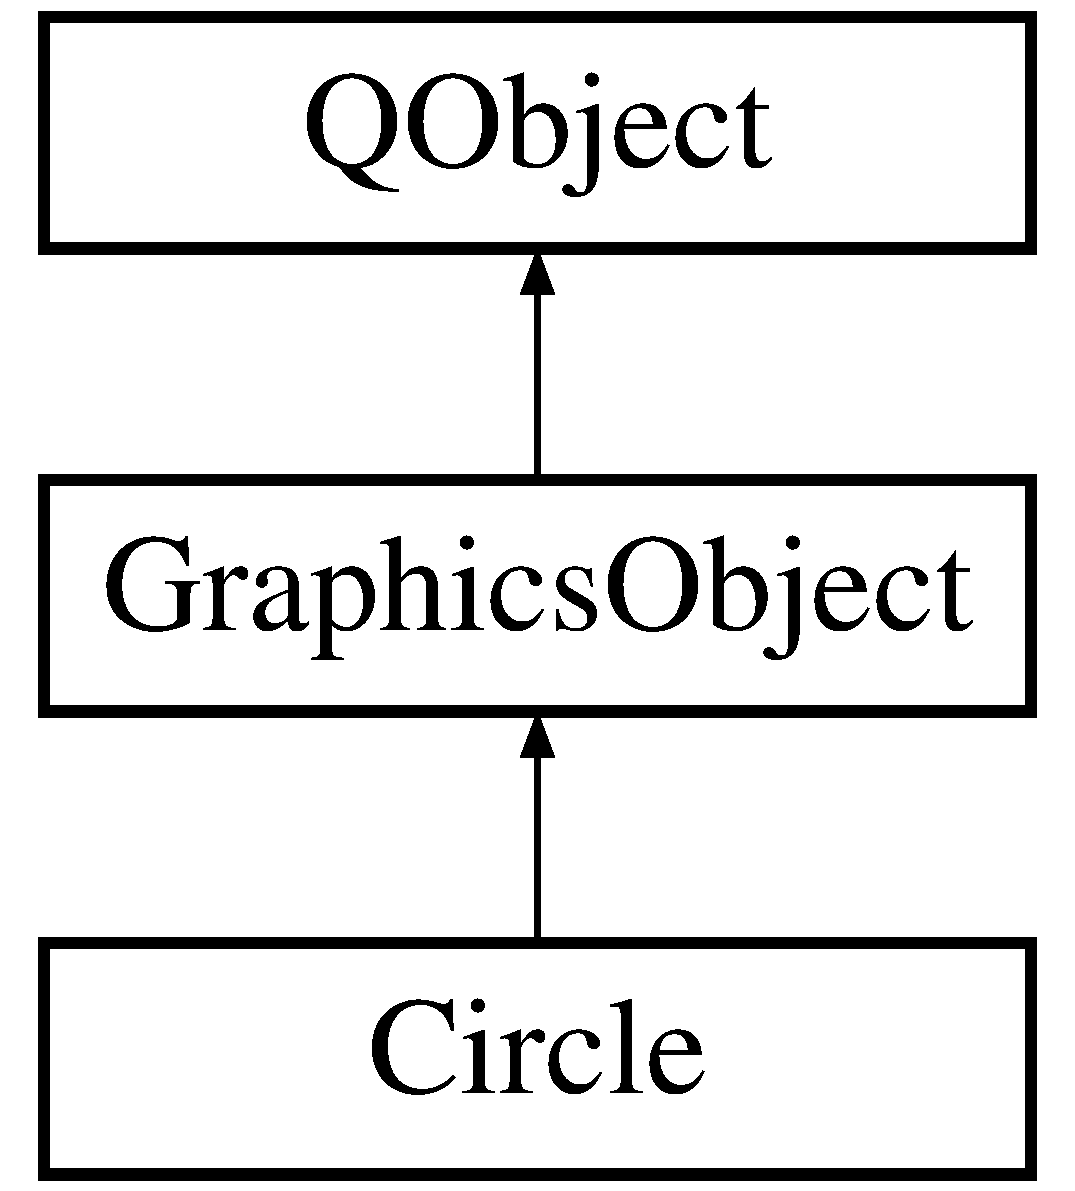
\includegraphics[height=3.000000cm]{class_circle}
\end{center}
\end{figure}
\subsection*{Public Member Functions}
\begin{DoxyCompactItemize}
\item 
\hyperlink{class_circle_a4dca54ed7e68a3cd4b4836deaa5ecea1}{Circle} (Q\+Object $\ast$parent=0)
\begin{DoxyCompactList}\small\item\em Generates a new \hyperlink{class_circle}{Circle} Object. \end{DoxyCompactList}\item 
virtual Q\+Graphics\+Item $\ast$ \hyperlink{class_circle_ad1fa0a922709e61b3e70eef604a3600d}{graphics\+Item} () const
\begin{DoxyCompactList}\small\item\em Graphics\+Item. \end{DoxyCompactList}\item 
\hyperlink{class_circle_a6c99dec4ddc0c9c289d4beaf2c4f9a9e}{Circle} (qreal x, qreal y, qreal width, qreal heigth, Q\+Color color1, Q\+Color color2)
\begin{DoxyCompactList}\small\item\em \hyperlink{class_circle_a4dca54ed7e68a3cd4b4836deaa5ecea1}{Circle\+::\+Circle}. \end{DoxyCompactList}\item 
Q\+String \hyperlink{class_circle_a2fea55f4310daa23eb8c103bdcdcabd6}{to\+String} ()
\end{DoxyCompactItemize}


\subsection{Detailed Description}
The \hyperlink{class_circle}{Circle} class. 

\subsection{Constructor \& Destructor Documentation}
\mbox{\Hypertarget{class_circle_a4dca54ed7e68a3cd4b4836deaa5ecea1}\label{class_circle_a4dca54ed7e68a3cd4b4836deaa5ecea1}} 
\index{Circle@{Circle}!Circle@{Circle}}
\index{Circle@{Circle}!Circle@{Circle}}
\subsubsection{\texorpdfstring{Circle()}{Circle()}\hspace{0.1cm}{\footnotesize\ttfamily [1/2]}}
{\footnotesize\ttfamily Circle\+::\+Circle (\begin{DoxyParamCaption}\item[{Q\+Object $\ast$}]{parent = {\ttfamily 0} }\end{DoxyParamCaption})\hspace{0.3cm}{\ttfamily [explicit]}}



Generates a new \hyperlink{class_circle}{Circle} Object. 


\begin{DoxyParams}{Parameters}
{\em parent} & \\
\hline
\end{DoxyParams}
\mbox{\Hypertarget{class_circle_a6c99dec4ddc0c9c289d4beaf2c4f9a9e}\label{class_circle_a6c99dec4ddc0c9c289d4beaf2c4f9a9e}} 
\index{Circle@{Circle}!Circle@{Circle}}
\index{Circle@{Circle}!Circle@{Circle}}
\subsubsection{\texorpdfstring{Circle()}{Circle()}\hspace{0.1cm}{\footnotesize\ttfamily [2/2]}}
{\footnotesize\ttfamily Circle\+::\+Circle (\begin{DoxyParamCaption}\item[{qreal}]{x,  }\item[{qreal}]{y,  }\item[{qreal}]{width,  }\item[{qreal}]{heigth,  }\item[{Q\+Color}]{color1,  }\item[{Q\+Color}]{color2 }\end{DoxyParamCaption})}



\hyperlink{class_circle_a4dca54ed7e68a3cd4b4836deaa5ecea1}{Circle\+::\+Circle}. 


\begin{DoxyParams}{Parameters}
{\em X-\/\+Position} & \\
\hline
{\em Y-\/\+Position} & \\
\hline
{\em Width} & \\
\hline
{\em Heigth} & \\
\hline
{\em color1} & \\
\hline
{\em color2} & \\
\hline
\end{DoxyParams}


\subsection{Member Function Documentation}
\mbox{\Hypertarget{class_circle_ad1fa0a922709e61b3e70eef604a3600d}\label{class_circle_ad1fa0a922709e61b3e70eef604a3600d}} 
\index{Circle@{Circle}!graphics\+Item@{graphics\+Item}}
\index{graphics\+Item@{graphics\+Item}!Circle@{Circle}}
\subsubsection{\texorpdfstring{graphics\+Item()}{graphicsItem()}}
{\footnotesize\ttfamily Q\+Graphics\+Item $\ast$ Circle\+::graphics\+Item (\begin{DoxyParamCaption}{ }\end{DoxyParamCaption}) const\hspace{0.3cm}{\ttfamily [virtual]}}



Graphics\+Item. 

\begin{DoxyReturn}{Returns}
Returns Ellipse 
\end{DoxyReturn}


Reimplemented from \hyperlink{class_graphics_object_abd625951730f006e748570bf00d158bf}{Graphics\+Object}.

\mbox{\Hypertarget{class_circle_a2fea55f4310daa23eb8c103bdcdcabd6}\label{class_circle_a2fea55f4310daa23eb8c103bdcdcabd6}} 
\index{Circle@{Circle}!to\+String@{to\+String}}
\index{to\+String@{to\+String}!Circle@{Circle}}
\subsubsection{\texorpdfstring{to\+String()}{toString()}}
{\footnotesize\ttfamily Q\+String Circle\+::to\+String (\begin{DoxyParamCaption}{ }\end{DoxyParamCaption})}



The documentation for this class was generated from the following files\+:\begin{DoxyCompactItemize}
\item 
\hyperlink{circle_8h}{circle.\+h}\item 
\hyperlink{circle_8cpp}{circle.\+cpp}\end{DoxyCompactItemize}

\hypertarget{class_color_button}{}\section{Color\+Button Class Reference}
\label{class_color_button}\index{Color\+Button@{Color\+Button}}


{\ttfamily \#include $<$colorbutton.\+h$>$}

Inheritance diagram for Color\+Button\+:\begin{figure}[H]
\begin{center}
\leavevmode
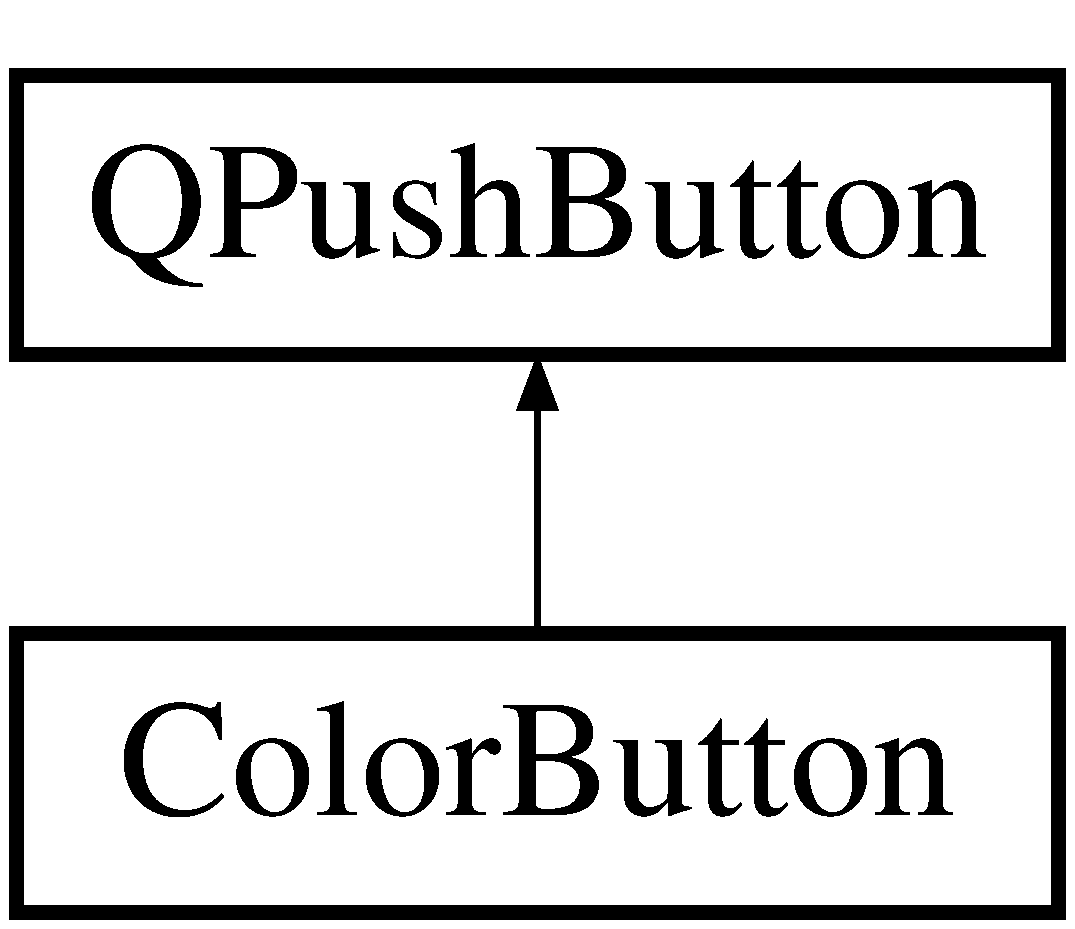
\includegraphics[height=2.000000cm]{class_color_button}
\end{center}
\end{figure}
\subsection*{Public Member Functions}
\begin{DoxyCompactItemize}
\item 
\hyperlink{class_color_button_a4b8e318941c5c69efd5a610fd7edb51e}{Color\+Button} ()
\item 
\hyperlink{class_color_button_a128b21900f22efdc9d71d0bffa0b64f8}{Color\+Button} (Q\+Widget $\ast$parent=0)
\item 
\hyperlink{class_color_button_a16f9cc31b3476fc5cb900e3692d4f49c}{Color\+Button} (Q\+Color \hyperlink{class_color_button_a7583a20c9a126ba93e344ea728c19954}{color}, Q\+Widget $\ast$parent=0)
\item 
Q\+Color \hyperlink{class_color_button_a7583a20c9a126ba93e344ea728c19954}{color} () const
\item 
void \hyperlink{class_color_button_ad0d3747c9ceb3ed57d3f513f42fd4cf2}{set\+Color} (const Q\+Color \&\hyperlink{class_color_button_a7583a20c9a126ba93e344ea728c19954}{color})
\end{DoxyCompactItemize}
\subsection*{Protected Member Functions}
\begin{DoxyCompactItemize}
\item 
void \hyperlink{class_color_button_ae7b2847c9974fb52f80d54dafc7a0f00}{paint\+Event} (Q\+Paint\+Event $\ast$)
\begin{DoxyCompactList}\small\item\em Overrides paint\+Event. Sets color to m\+\_\+color. \end{DoxyCompactList}\end{DoxyCompactItemize}
\subsection*{Protected Attributes}
\begin{DoxyCompactItemize}
\item 
Q\+Color \hyperlink{class_color_button_aa4408cd251575659e5e8417802f276e4}{m\+\_\+color}
\end{DoxyCompactItemize}


\subsection{Constructor \& Destructor Documentation}
\mbox{\Hypertarget{class_color_button_a4b8e318941c5c69efd5a610fd7edb51e}\label{class_color_button_a4b8e318941c5c69efd5a610fd7edb51e}} 
\index{Color\+Button@{Color\+Button}!Color\+Button@{Color\+Button}}
\index{Color\+Button@{Color\+Button}!Color\+Button@{Color\+Button}}
\subsubsection{\texorpdfstring{Color\+Button()}{ColorButton()}\hspace{0.1cm}{\footnotesize\ttfamily [1/3]}}
{\footnotesize\ttfamily Color\+Button\+::\+Color\+Button (\begin{DoxyParamCaption}{ }\end{DoxyParamCaption})}

\mbox{\Hypertarget{class_color_button_a128b21900f22efdc9d71d0bffa0b64f8}\label{class_color_button_a128b21900f22efdc9d71d0bffa0b64f8}} 
\index{Color\+Button@{Color\+Button}!Color\+Button@{Color\+Button}}
\index{Color\+Button@{Color\+Button}!Color\+Button@{Color\+Button}}
\subsubsection{\texorpdfstring{Color\+Button()}{ColorButton()}\hspace{0.1cm}{\footnotesize\ttfamily [2/3]}}
{\footnotesize\ttfamily Color\+Button\+::\+Color\+Button (\begin{DoxyParamCaption}\item[{Q\+Widget $\ast$}]{parent = {\ttfamily 0} }\end{DoxyParamCaption})}

\mbox{\Hypertarget{class_color_button_a16f9cc31b3476fc5cb900e3692d4f49c}\label{class_color_button_a16f9cc31b3476fc5cb900e3692d4f49c}} 
\index{Color\+Button@{Color\+Button}!Color\+Button@{Color\+Button}}
\index{Color\+Button@{Color\+Button}!Color\+Button@{Color\+Button}}
\subsubsection{\texorpdfstring{Color\+Button()}{ColorButton()}\hspace{0.1cm}{\footnotesize\ttfamily [3/3]}}
{\footnotesize\ttfamily Color\+Button\+::\+Color\+Button (\begin{DoxyParamCaption}\item[{Q\+Color}]{color,  }\item[{Q\+Widget $\ast$}]{parent = {\ttfamily 0} }\end{DoxyParamCaption})}



\subsection{Member Function Documentation}
\mbox{\Hypertarget{class_color_button_a7583a20c9a126ba93e344ea728c19954}\label{class_color_button_a7583a20c9a126ba93e344ea728c19954}} 
\index{Color\+Button@{Color\+Button}!color@{color}}
\index{color@{color}!Color\+Button@{Color\+Button}}
\subsubsection{\texorpdfstring{color()}{color()}}
{\footnotesize\ttfamily Q\+Color Color\+Button\+::color (\begin{DoxyParamCaption}{ }\end{DoxyParamCaption}) const}

\mbox{\Hypertarget{class_color_button_ae7b2847c9974fb52f80d54dafc7a0f00}\label{class_color_button_ae7b2847c9974fb52f80d54dafc7a0f00}} 
\index{Color\+Button@{Color\+Button}!paint\+Event@{paint\+Event}}
\index{paint\+Event@{paint\+Event}!Color\+Button@{Color\+Button}}
\subsubsection{\texorpdfstring{paint\+Event()}{paintEvent()}}
{\footnotesize\ttfamily void Color\+Button\+::paint\+Event (\begin{DoxyParamCaption}\item[{Q\+Paint\+Event $\ast$}]{paint }\end{DoxyParamCaption})\hspace{0.3cm}{\ttfamily [protected]}}



Overrides paint\+Event. Sets color to m\+\_\+color. 


\begin{DoxyParams}{Parameters}
{\em paint} & \\
\hline
\end{DoxyParams}
\mbox{\Hypertarget{class_color_button_ad0d3747c9ceb3ed57d3f513f42fd4cf2}\label{class_color_button_ad0d3747c9ceb3ed57d3f513f42fd4cf2}} 
\index{Color\+Button@{Color\+Button}!set\+Color@{set\+Color}}
\index{set\+Color@{set\+Color}!Color\+Button@{Color\+Button}}
\subsubsection{\texorpdfstring{set\+Color()}{setColor()}}
{\footnotesize\ttfamily void Color\+Button\+::set\+Color (\begin{DoxyParamCaption}\item[{const Q\+Color \&}]{color }\end{DoxyParamCaption})}



\subsection{Member Data Documentation}
\mbox{\Hypertarget{class_color_button_aa4408cd251575659e5e8417802f276e4}\label{class_color_button_aa4408cd251575659e5e8417802f276e4}} 
\index{Color\+Button@{Color\+Button}!m\+\_\+color@{m\+\_\+color}}
\index{m\+\_\+color@{m\+\_\+color}!Color\+Button@{Color\+Button}}
\subsubsection{\texorpdfstring{m\+\_\+color}{m\_color}}
{\footnotesize\ttfamily Q\+Color Color\+Button\+::m\+\_\+color\hspace{0.3cm}{\ttfamily [protected]}}



The documentation for this class was generated from the following files\+:\begin{DoxyCompactItemize}
\item 
\hyperlink{colorbutton_8h}{colorbutton.\+h}\item 
\hyperlink{colorbutton_8cpp}{colorbutton.\+cpp}\end{DoxyCompactItemize}

\hypertarget{class_color_tool_selector}{}\section{Color\+Tool\+Selector Class Reference}
\label{class_color_tool_selector}\index{Color\+Tool\+Selector@{Color\+Tool\+Selector}}


{\ttfamily \#include $<$colortoolselector.\+h$>$}

Inheritance diagram for Color\+Tool\+Selector\+:\begin{figure}[H]
\begin{center}
\leavevmode
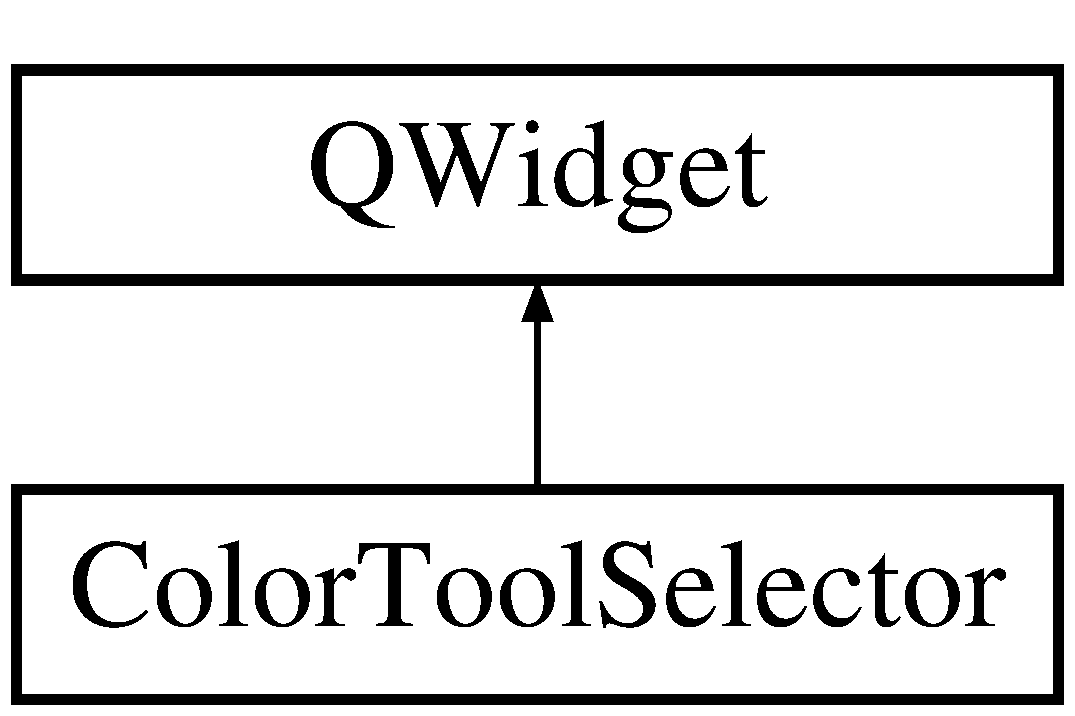
\includegraphics[height=2.000000cm]{class_color_tool_selector}
\end{center}
\end{figure}
\subsection*{Signals}
\begin{DoxyCompactItemize}
\item 
void \hyperlink{class_color_tool_selector_a36ab517be160748460a07eb0599023f6}{active\+Fill\+Color\+Tool\+Changed} (Q\+Color \hyperlink{class_color_tool_selector_ad1976b1daefca06700111da01edff3d4}{fill\+Color})
\item 
void \hyperlink{class_color_tool_selector_acfb60e1e55b31e4d784feab0552874d2}{active\+Border\+Color\+Tool\+Changed} (Q\+Color \hyperlink{class_color_tool_selector_ad1976b1daefca06700111da01edff3d4}{fill\+Color})
\end{DoxyCompactItemize}
\subsection*{Public Member Functions}
\begin{DoxyCompactItemize}
\item 
\hyperlink{class_color_tool_selector_a42acf2fbc6dea5c4575ed166f3362c92}{Color\+Tool\+Selector} (Q\+Widget $\ast$parent=0)
\item 
\hyperlink{class_color_tool_selector_a461eb04b3d3d25bee5bb5848488f0b0d}{$\sim$\+Color\+Tool\+Selector} ()
\item 
Q\+Color \hyperlink{class_color_tool_selector_ad1976b1daefca06700111da01edff3d4}{fill\+Color} () const
\end{DoxyCompactItemize}
\subsection*{Protected Attributes}
\begin{DoxyCompactItemize}
\item 
\hyperlink{class_draw}{Draw} $\ast$ \hyperlink{class_color_tool_selector_af2464293935f4a53d1cbcc3b0596823d}{m\+\_\+draw}
\end{DoxyCompactItemize}


\subsection{Constructor \& Destructor Documentation}
\mbox{\Hypertarget{class_color_tool_selector_a42acf2fbc6dea5c4575ed166f3362c92}\label{class_color_tool_selector_a42acf2fbc6dea5c4575ed166f3362c92}} 
\index{Color\+Tool\+Selector@{Color\+Tool\+Selector}!Color\+Tool\+Selector@{Color\+Tool\+Selector}}
\index{Color\+Tool\+Selector@{Color\+Tool\+Selector}!Color\+Tool\+Selector@{Color\+Tool\+Selector}}
\subsubsection{\texorpdfstring{Color\+Tool\+Selector()}{ColorToolSelector()}}
{\footnotesize\ttfamily Color\+Tool\+Selector\+::\+Color\+Tool\+Selector (\begin{DoxyParamCaption}\item[{Q\+Widget $\ast$}]{parent = {\ttfamily 0} }\end{DoxyParamCaption})\hspace{0.3cm}{\ttfamily [explicit]}}

\mbox{\Hypertarget{class_color_tool_selector_a461eb04b3d3d25bee5bb5848488f0b0d}\label{class_color_tool_selector_a461eb04b3d3d25bee5bb5848488f0b0d}} 
\index{Color\+Tool\+Selector@{Color\+Tool\+Selector}!````~Color\+Tool\+Selector@{$\sim$\+Color\+Tool\+Selector}}
\index{````~Color\+Tool\+Selector@{$\sim$\+Color\+Tool\+Selector}!Color\+Tool\+Selector@{Color\+Tool\+Selector}}
\subsubsection{\texorpdfstring{$\sim$\+Color\+Tool\+Selector()}{~ColorToolSelector()}}
{\footnotesize\ttfamily Color\+Tool\+Selector\+::$\sim$\+Color\+Tool\+Selector (\begin{DoxyParamCaption}{ }\end{DoxyParamCaption})}



\subsection{Member Function Documentation}
\mbox{\Hypertarget{class_color_tool_selector_acfb60e1e55b31e4d784feab0552874d2}\label{class_color_tool_selector_acfb60e1e55b31e4d784feab0552874d2}} 
\index{Color\+Tool\+Selector@{Color\+Tool\+Selector}!active\+Border\+Color\+Tool\+Changed@{active\+Border\+Color\+Tool\+Changed}}
\index{active\+Border\+Color\+Tool\+Changed@{active\+Border\+Color\+Tool\+Changed}!Color\+Tool\+Selector@{Color\+Tool\+Selector}}
\subsubsection{\texorpdfstring{active\+Border\+Color\+Tool\+Changed}{activeBorderColorToolChanged}}
{\footnotesize\ttfamily void Color\+Tool\+Selector\+::active\+Border\+Color\+Tool\+Changed (\begin{DoxyParamCaption}\item[{Q\+Color}]{fill\+Color }\end{DoxyParamCaption})\hspace{0.3cm}{\ttfamily [signal]}}

\mbox{\Hypertarget{class_color_tool_selector_a36ab517be160748460a07eb0599023f6}\label{class_color_tool_selector_a36ab517be160748460a07eb0599023f6}} 
\index{Color\+Tool\+Selector@{Color\+Tool\+Selector}!active\+Fill\+Color\+Tool\+Changed@{active\+Fill\+Color\+Tool\+Changed}}
\index{active\+Fill\+Color\+Tool\+Changed@{active\+Fill\+Color\+Tool\+Changed}!Color\+Tool\+Selector@{Color\+Tool\+Selector}}
\subsubsection{\texorpdfstring{active\+Fill\+Color\+Tool\+Changed}{activeFillColorToolChanged}}
{\footnotesize\ttfamily void Color\+Tool\+Selector\+::active\+Fill\+Color\+Tool\+Changed (\begin{DoxyParamCaption}\item[{Q\+Color}]{fill\+Color }\end{DoxyParamCaption})\hspace{0.3cm}{\ttfamily [signal]}}

\mbox{\Hypertarget{class_color_tool_selector_ad1976b1daefca06700111da01edff3d4}\label{class_color_tool_selector_ad1976b1daefca06700111da01edff3d4}} 
\index{Color\+Tool\+Selector@{Color\+Tool\+Selector}!fill\+Color@{fill\+Color}}
\index{fill\+Color@{fill\+Color}!Color\+Tool\+Selector@{Color\+Tool\+Selector}}
\subsubsection{\texorpdfstring{fill\+Color()}{fillColor()}}
{\footnotesize\ttfamily Q\+Color Color\+Tool\+Selector\+::fill\+Color (\begin{DoxyParamCaption}{ }\end{DoxyParamCaption}) const}



\subsection{Member Data Documentation}
\mbox{\Hypertarget{class_color_tool_selector_af2464293935f4a53d1cbcc3b0596823d}\label{class_color_tool_selector_af2464293935f4a53d1cbcc3b0596823d}} 
\index{Color\+Tool\+Selector@{Color\+Tool\+Selector}!m\+\_\+draw@{m\+\_\+draw}}
\index{m\+\_\+draw@{m\+\_\+draw}!Color\+Tool\+Selector@{Color\+Tool\+Selector}}
\subsubsection{\texorpdfstring{m\+\_\+draw}{m\_draw}}
{\footnotesize\ttfamily \hyperlink{class_draw}{Draw}$\ast$ Color\+Tool\+Selector\+::m\+\_\+draw\hspace{0.3cm}{\ttfamily [protected]}}



The documentation for this class was generated from the following files\+:\begin{DoxyCompactItemize}
\item 
\hyperlink{colortoolselector_8h}{colortoolselector.\+h}\item 
\hyperlink{colortoolselector_8cpp}{colortoolselector.\+cpp}\end{DoxyCompactItemize}

\hypertarget{class_ui_1_1_color_tool_selector}{}\section{Ui\+:\+:Color\+Tool\+Selector Class Reference}
\label{class_ui_1_1_color_tool_selector}\index{Ui\+::\+Color\+Tool\+Selector@{Ui\+::\+Color\+Tool\+Selector}}


{\ttfamily \#include $<$ui\+\_\+colortoolselector.\+h$>$}

Inheritance diagram for Ui\+:\+:Color\+Tool\+Selector\+:\begin{figure}[H]
\begin{center}
\leavevmode
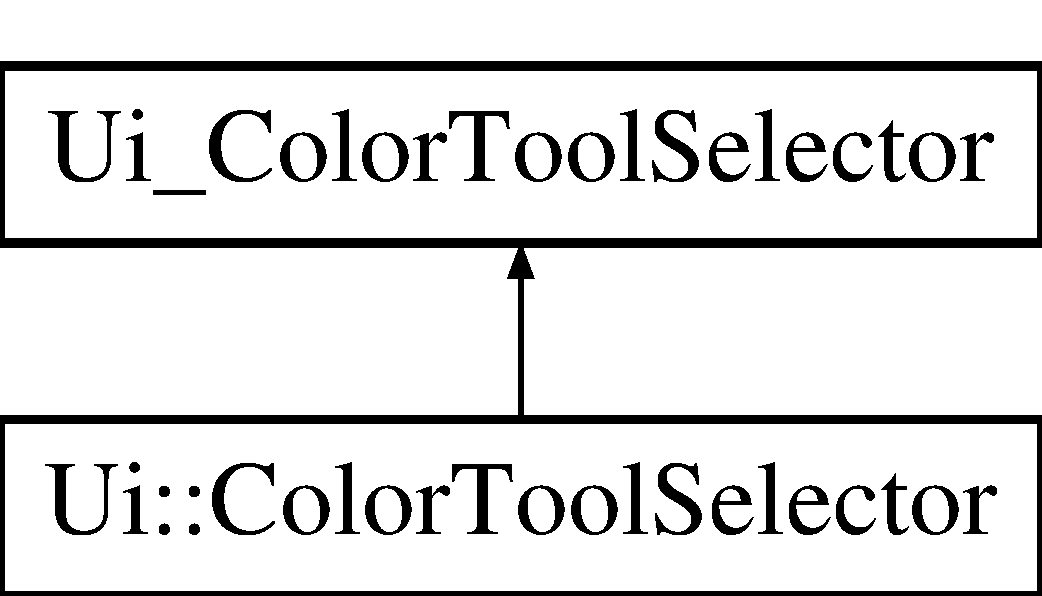
\includegraphics[height=2.000000cm]{class_ui_1_1_color_tool_selector}
\end{center}
\end{figure}
\subsection*{Additional Inherited Members}


The documentation for this class was generated from the following file\+:\begin{DoxyCompactItemize}
\item 
\hyperlink{ui__colortoolselector_8h}{ui\+\_\+colortoolselector.\+h}\end{DoxyCompactItemize}

\hypertarget{class_draw}{}\section{Draw Class Reference}
\label{class_draw}\index{Draw@{Draw}}


{\ttfamily \#include $<$draw.\+h$>$}

Inheritance diagram for Draw\+:\begin{figure}[H]
\begin{center}
\leavevmode
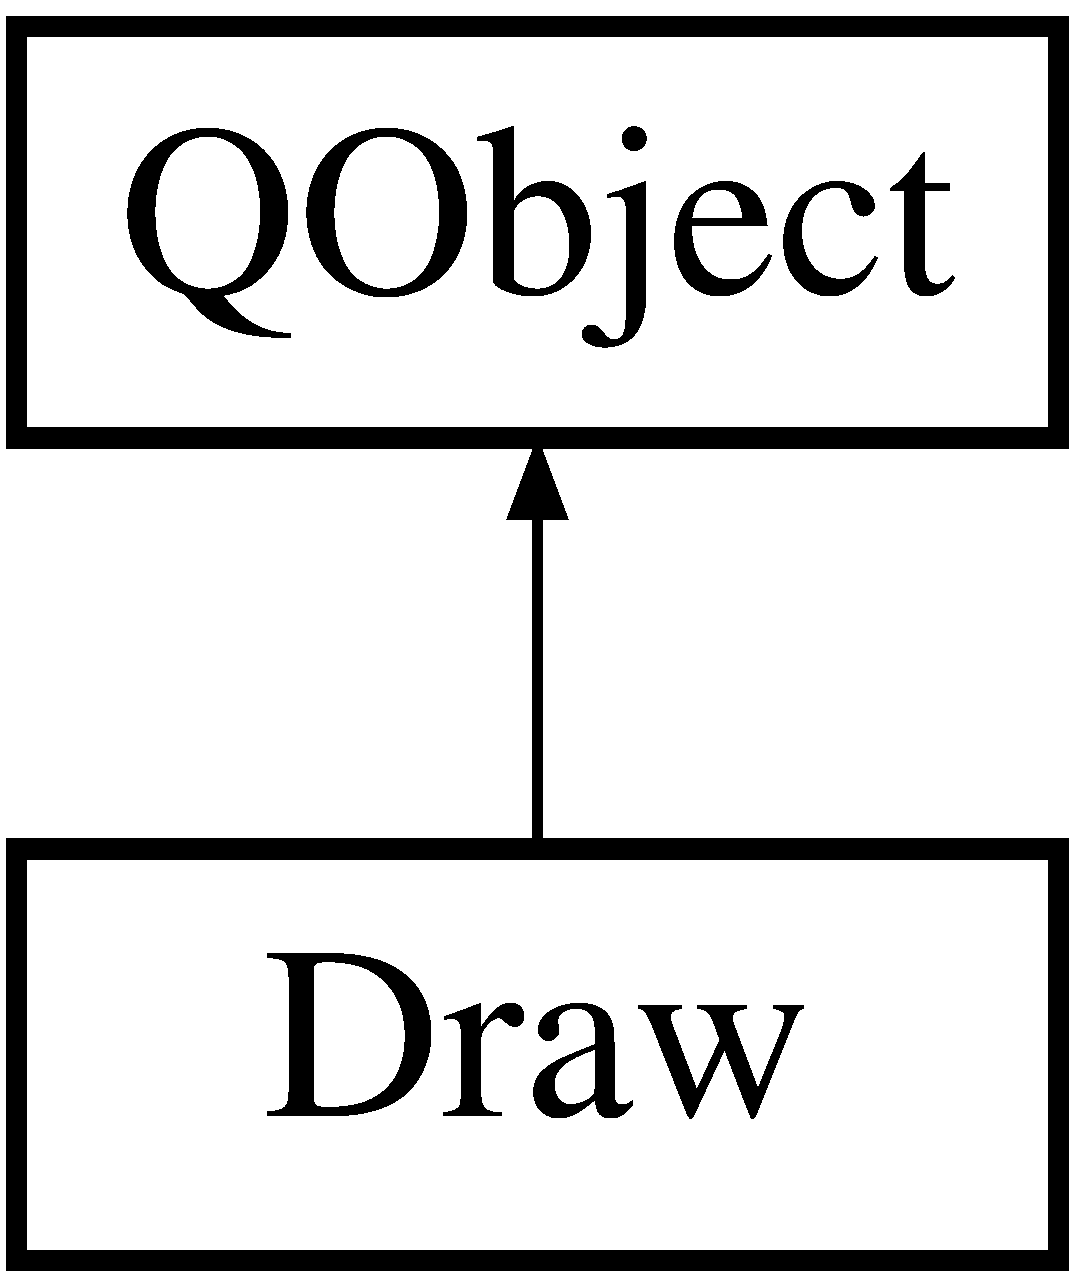
\includegraphics[height=2.000000cm]{class_draw}
\end{center}
\end{figure}
\subsection*{Public Types}
\begin{DoxyCompactItemize}
\item 
enum \hyperlink{class_draw_aef97a848de7a634c35c3ce678be88b9b}{Tool} \{ \hyperlink{class_draw_aef97a848de7a634c35c3ce678be88b9bae4a005b9e5843075e8e0a77b7a3d7159}{select\+Tool}, 
\hyperlink{class_draw_aef97a848de7a634c35c3ce678be88b9ba28e42983eabb4d975227fb7b365c3295}{line\+Tool}, 
\hyperlink{class_draw_aef97a848de7a634c35c3ce678be88b9baf76785749efd3ceaf7fa226d8cc0de66}{circle\+Tool}, 
\hyperlink{class_draw_aef97a848de7a634c35c3ce678be88b9ba7778b9c2175c8a25f395a1565c5dac30}{rect\+Tool}
 \}
\end{DoxyCompactItemize}
\subsection*{Public Slots}
\begin{DoxyCompactItemize}
\item 
void \hyperlink{class_draw_a960270765705698a6663fdfe93356d17}{set\+Border\+Color} (const Q\+Color \&value)
\begin{DoxyCompactList}\small\item\em \hyperlink{class_draw_a960270765705698a6663fdfe93356d17}{Draw\+::set\+Border\+Color}. \end{DoxyCompactList}\item 
void \hyperlink{class_draw_a7d802038dd6aa2afe1a8570dbe681136}{set\+Fill\+Color} (const Q\+Color \&value)
\begin{DoxyCompactList}\small\item\em \hyperlink{class_draw_a7d802038dd6aa2afe1a8570dbe681136}{Draw\+::set\+Fill\+Color}. \end{DoxyCompactList}\item 
void \hyperlink{class_draw_af955c348f57d49fdb861ad82f485b902}{setT} (const \hyperlink{class_draw_aef97a848de7a634c35c3ce678be88b9b}{Draw\+::\+Tool} \&t)
\begin{DoxyCompactList}\small\item\em \hyperlink{class_draw_af955c348f57d49fdb861ad82f485b902}{Draw\+::setT}. \end{DoxyCompactList}\end{DoxyCompactItemize}
\subsection*{Signals}
\begin{DoxyCompactItemize}
\item 
void \hyperlink{class_draw_a65056d377baf1383f8af678ba2ed1467}{active\+Drawing\+Tool\+Changed} (\hyperlink{class_draw_aef97a848de7a634c35c3ce678be88b9b}{Draw\+::\+Tool} active\+Drawing\+Tool)
\item 
void \hyperlink{class_draw_ac28b7e408c687ddfd85e01954109329d}{active\+Fill\+Color\+Tool\+Changed} (Q\+Color fill\+Color)
\item 
void \hyperlink{class_draw_aeafc6ac98a670e97b047bc34d7a13141}{active\+Border\+Color\+Tool\+Changed} (Q\+Color border\+Color)
\end{DoxyCompactItemize}
\subsection*{Public Member Functions}
\begin{DoxyCompactItemize}
\item 
\hyperlink{class_draw_aaad70829cedc40ada59d620bf075e27d}{Draw} (Q\+Object $\ast$parent=0)
\begin{DoxyCompactList}\small\item\em \hyperlink{class_draw_aaad70829cedc40ada59d620bf075e27d}{Draw\+::\+Draw}. \end{DoxyCompactList}\item 
Q\+Color \hyperlink{class_draw_aa3700cc975270d70dcf18d4160d7f1e6}{get\+Border\+Color} () const
\begin{DoxyCompactList}\small\item\em \hyperlink{class_draw_aa3700cc975270d70dcf18d4160d7f1e6}{Draw\+::get\+Border\+Color}. \end{DoxyCompactList}\item 
Q\+Color \hyperlink{class_draw_a4be8a242b92fd9d5c42fe9a40810cdb6}{get\+Fill\+Color} () const
\begin{DoxyCompactList}\small\item\em \hyperlink{class_draw_a4be8a242b92fd9d5c42fe9a40810cdb6}{Draw\+::get\+Fill\+Color}. \end{DoxyCompactList}\item 
\hyperlink{class_draw_aef97a848de7a634c35c3ce678be88b9b}{Draw\+::\+Tool} \hyperlink{class_draw_a051a72609a03e7b21990060d0f306558}{getT} () const
\begin{DoxyCompactList}\small\item\em \hyperlink{class_draw_a051a72609a03e7b21990060d0f306558}{Draw\+::getT}. \end{DoxyCompactList}\end{DoxyCompactItemize}


\subsection{Member Enumeration Documentation}
\mbox{\Hypertarget{class_draw_aef97a848de7a634c35c3ce678be88b9b}\label{class_draw_aef97a848de7a634c35c3ce678be88b9b}} 
\index{Draw@{Draw}!Tool@{Tool}}
\index{Tool@{Tool}!Draw@{Draw}}
\subsubsection{\texorpdfstring{Tool}{Tool}}
{\footnotesize\ttfamily enum \hyperlink{class_draw_aef97a848de7a634c35c3ce678be88b9b}{Draw\+::\+Tool}}

\begin{DoxyEnumFields}{Enumerator}
\raisebox{\heightof{T}}[0pt][0pt]{\index{select\+Tool@{select\+Tool}!Draw@{Draw}}\index{Draw@{Draw}!select\+Tool@{select\+Tool}}}\mbox{\Hypertarget{class_draw_aef97a848de7a634c35c3ce678be88b9bae4a005b9e5843075e8e0a77b7a3d7159}\label{class_draw_aef97a848de7a634c35c3ce678be88b9bae4a005b9e5843075e8e0a77b7a3d7159}} 
select\+Tool&\\
\hline

\raisebox{\heightof{T}}[0pt][0pt]{\index{line\+Tool@{line\+Tool}!Draw@{Draw}}\index{Draw@{Draw}!line\+Tool@{line\+Tool}}}\mbox{\Hypertarget{class_draw_aef97a848de7a634c35c3ce678be88b9ba28e42983eabb4d975227fb7b365c3295}\label{class_draw_aef97a848de7a634c35c3ce678be88b9ba28e42983eabb4d975227fb7b365c3295}} 
line\+Tool&\\
\hline

\raisebox{\heightof{T}}[0pt][0pt]{\index{circle\+Tool@{circle\+Tool}!Draw@{Draw}}\index{Draw@{Draw}!circle\+Tool@{circle\+Tool}}}\mbox{\Hypertarget{class_draw_aef97a848de7a634c35c3ce678be88b9baf76785749efd3ceaf7fa226d8cc0de66}\label{class_draw_aef97a848de7a634c35c3ce678be88b9baf76785749efd3ceaf7fa226d8cc0de66}} 
circle\+Tool&\\
\hline

\raisebox{\heightof{T}}[0pt][0pt]{\index{rect\+Tool@{rect\+Tool}!Draw@{Draw}}\index{Draw@{Draw}!rect\+Tool@{rect\+Tool}}}\mbox{\Hypertarget{class_draw_aef97a848de7a634c35c3ce678be88b9ba7778b9c2175c8a25f395a1565c5dac30}\label{class_draw_aef97a848de7a634c35c3ce678be88b9ba7778b9c2175c8a25f395a1565c5dac30}} 
rect\+Tool&\\
\hline

\end{DoxyEnumFields}


\subsection{Constructor \& Destructor Documentation}
\mbox{\Hypertarget{class_draw_aaad70829cedc40ada59d620bf075e27d}\label{class_draw_aaad70829cedc40ada59d620bf075e27d}} 
\index{Draw@{Draw}!Draw@{Draw}}
\index{Draw@{Draw}!Draw@{Draw}}
\subsubsection{\texorpdfstring{Draw()}{Draw()}}
{\footnotesize\ttfamily Draw\+::\+Draw (\begin{DoxyParamCaption}\item[{Q\+Object $\ast$}]{parent = {\ttfamily 0} }\end{DoxyParamCaption})\hspace{0.3cm}{\ttfamily [explicit]}}



\hyperlink{class_draw_aaad70829cedc40ada59d620bf075e27d}{Draw\+::\+Draw}. 


\begin{DoxyParams}{Parameters}
{\em parent} & \\
\hline
\end{DoxyParams}


\subsection{Member Function Documentation}
\mbox{\Hypertarget{class_draw_aeafc6ac98a670e97b047bc34d7a13141}\label{class_draw_aeafc6ac98a670e97b047bc34d7a13141}} 
\index{Draw@{Draw}!active\+Border\+Color\+Tool\+Changed@{active\+Border\+Color\+Tool\+Changed}}
\index{active\+Border\+Color\+Tool\+Changed@{active\+Border\+Color\+Tool\+Changed}!Draw@{Draw}}
\subsubsection{\texorpdfstring{active\+Border\+Color\+Tool\+Changed}{activeBorderColorToolChanged}}
{\footnotesize\ttfamily void Draw\+::active\+Border\+Color\+Tool\+Changed (\begin{DoxyParamCaption}\item[{Q\+Color}]{border\+Color }\end{DoxyParamCaption})\hspace{0.3cm}{\ttfamily [signal]}}

\mbox{\Hypertarget{class_draw_a65056d377baf1383f8af678ba2ed1467}\label{class_draw_a65056d377baf1383f8af678ba2ed1467}} 
\index{Draw@{Draw}!active\+Drawing\+Tool\+Changed@{active\+Drawing\+Tool\+Changed}}
\index{active\+Drawing\+Tool\+Changed@{active\+Drawing\+Tool\+Changed}!Draw@{Draw}}
\subsubsection{\texorpdfstring{active\+Drawing\+Tool\+Changed}{activeDrawingToolChanged}}
{\footnotesize\ttfamily void Draw\+::active\+Drawing\+Tool\+Changed (\begin{DoxyParamCaption}\item[{\hyperlink{class_draw_aef97a848de7a634c35c3ce678be88b9b}{Draw\+::\+Tool}}]{active\+Drawing\+Tool }\end{DoxyParamCaption})\hspace{0.3cm}{\ttfamily [signal]}}

\mbox{\Hypertarget{class_draw_ac28b7e408c687ddfd85e01954109329d}\label{class_draw_ac28b7e408c687ddfd85e01954109329d}} 
\index{Draw@{Draw}!active\+Fill\+Color\+Tool\+Changed@{active\+Fill\+Color\+Tool\+Changed}}
\index{active\+Fill\+Color\+Tool\+Changed@{active\+Fill\+Color\+Tool\+Changed}!Draw@{Draw}}
\subsubsection{\texorpdfstring{active\+Fill\+Color\+Tool\+Changed}{activeFillColorToolChanged}}
{\footnotesize\ttfamily void Draw\+::active\+Fill\+Color\+Tool\+Changed (\begin{DoxyParamCaption}\item[{Q\+Color}]{fill\+Color }\end{DoxyParamCaption})\hspace{0.3cm}{\ttfamily [signal]}}

\mbox{\Hypertarget{class_draw_aa3700cc975270d70dcf18d4160d7f1e6}\label{class_draw_aa3700cc975270d70dcf18d4160d7f1e6}} 
\index{Draw@{Draw}!get\+Border\+Color@{get\+Border\+Color}}
\index{get\+Border\+Color@{get\+Border\+Color}!Draw@{Draw}}
\subsubsection{\texorpdfstring{get\+Border\+Color()}{getBorderColor()}}
{\footnotesize\ttfamily Q\+Color Draw\+::get\+Border\+Color (\begin{DoxyParamCaption}{ }\end{DoxyParamCaption}) const}



\hyperlink{class_draw_aa3700cc975270d70dcf18d4160d7f1e6}{Draw\+::get\+Border\+Color}. 

\begin{DoxyReturn}{Returns}

\end{DoxyReturn}
\mbox{\Hypertarget{class_draw_a4be8a242b92fd9d5c42fe9a40810cdb6}\label{class_draw_a4be8a242b92fd9d5c42fe9a40810cdb6}} 
\index{Draw@{Draw}!get\+Fill\+Color@{get\+Fill\+Color}}
\index{get\+Fill\+Color@{get\+Fill\+Color}!Draw@{Draw}}
\subsubsection{\texorpdfstring{get\+Fill\+Color()}{getFillColor()}}
{\footnotesize\ttfamily Q\+Color Draw\+::get\+Fill\+Color (\begin{DoxyParamCaption}{ }\end{DoxyParamCaption}) const}



\hyperlink{class_draw_a4be8a242b92fd9d5c42fe9a40810cdb6}{Draw\+::get\+Fill\+Color}. 

\begin{DoxyReturn}{Returns}

\end{DoxyReturn}
\mbox{\Hypertarget{class_draw_a051a72609a03e7b21990060d0f306558}\label{class_draw_a051a72609a03e7b21990060d0f306558}} 
\index{Draw@{Draw}!getT@{getT}}
\index{getT@{getT}!Draw@{Draw}}
\subsubsection{\texorpdfstring{get\+T()}{getT()}}
{\footnotesize\ttfamily \hyperlink{class_draw_aef97a848de7a634c35c3ce678be88b9b}{Draw\+::\+Tool} Draw\+::getT (\begin{DoxyParamCaption}{ }\end{DoxyParamCaption}) const}



\hyperlink{class_draw_a051a72609a03e7b21990060d0f306558}{Draw\+::getT}. 

\begin{DoxyReturn}{Returns}

\end{DoxyReturn}
\mbox{\Hypertarget{class_draw_a960270765705698a6663fdfe93356d17}\label{class_draw_a960270765705698a6663fdfe93356d17}} 
\index{Draw@{Draw}!set\+Border\+Color@{set\+Border\+Color}}
\index{set\+Border\+Color@{set\+Border\+Color}!Draw@{Draw}}
\subsubsection{\texorpdfstring{set\+Border\+Color}{setBorderColor}}
{\footnotesize\ttfamily void Draw\+::set\+Border\+Color (\begin{DoxyParamCaption}\item[{const Q\+Color \&}]{value }\end{DoxyParamCaption})\hspace{0.3cm}{\ttfamily [slot]}}



\hyperlink{class_draw_a960270765705698a6663fdfe93356d17}{Draw\+::set\+Border\+Color}. 


\begin{DoxyParams}{Parameters}
{\em value} & \\
\hline
\end{DoxyParams}
\mbox{\Hypertarget{class_draw_a7d802038dd6aa2afe1a8570dbe681136}\label{class_draw_a7d802038dd6aa2afe1a8570dbe681136}} 
\index{Draw@{Draw}!set\+Fill\+Color@{set\+Fill\+Color}}
\index{set\+Fill\+Color@{set\+Fill\+Color}!Draw@{Draw}}
\subsubsection{\texorpdfstring{set\+Fill\+Color}{setFillColor}}
{\footnotesize\ttfamily void Draw\+::set\+Fill\+Color (\begin{DoxyParamCaption}\item[{const Q\+Color \&}]{value }\end{DoxyParamCaption})\hspace{0.3cm}{\ttfamily [slot]}}



\hyperlink{class_draw_a7d802038dd6aa2afe1a8570dbe681136}{Draw\+::set\+Fill\+Color}. 


\begin{DoxyParams}{Parameters}
{\em value} & \\
\hline
\end{DoxyParams}
\mbox{\Hypertarget{class_draw_af955c348f57d49fdb861ad82f485b902}\label{class_draw_af955c348f57d49fdb861ad82f485b902}} 
\index{Draw@{Draw}!setT@{setT}}
\index{setT@{setT}!Draw@{Draw}}
\subsubsection{\texorpdfstring{setT}{setT}}
{\footnotesize\ttfamily void Draw\+::setT (\begin{DoxyParamCaption}\item[{const \hyperlink{class_draw_aef97a848de7a634c35c3ce678be88b9b}{Draw\+::\+Tool} \&}]{t }\end{DoxyParamCaption})\hspace{0.3cm}{\ttfamily [slot]}}



\hyperlink{class_draw_af955c348f57d49fdb861ad82f485b902}{Draw\+::setT}. 


\begin{DoxyParams}{Parameters}
{\em t} & \\
\hline
\end{DoxyParams}


The documentation for this class was generated from the following files\+:\begin{DoxyCompactItemize}
\item 
\hyperlink{draw_8h}{draw.\+h}\item 
\hyperlink{draw_8cpp}{draw.\+cpp}\end{DoxyCompactItemize}

\hypertarget{class_ui_1_1_drawing_tool_selector}{}\section{Ui\+:\+:Drawing\+Tool\+Selector Class Reference}
\label{class_ui_1_1_drawing_tool_selector}\index{Ui\+::\+Drawing\+Tool\+Selector@{Ui\+::\+Drawing\+Tool\+Selector}}


{\ttfamily \#include $<$ui\+\_\+drawingtoolselector.\+h$>$}

Inheritance diagram for Ui\+:\+:Drawing\+Tool\+Selector\+:\begin{figure}[H]
\begin{center}
\leavevmode
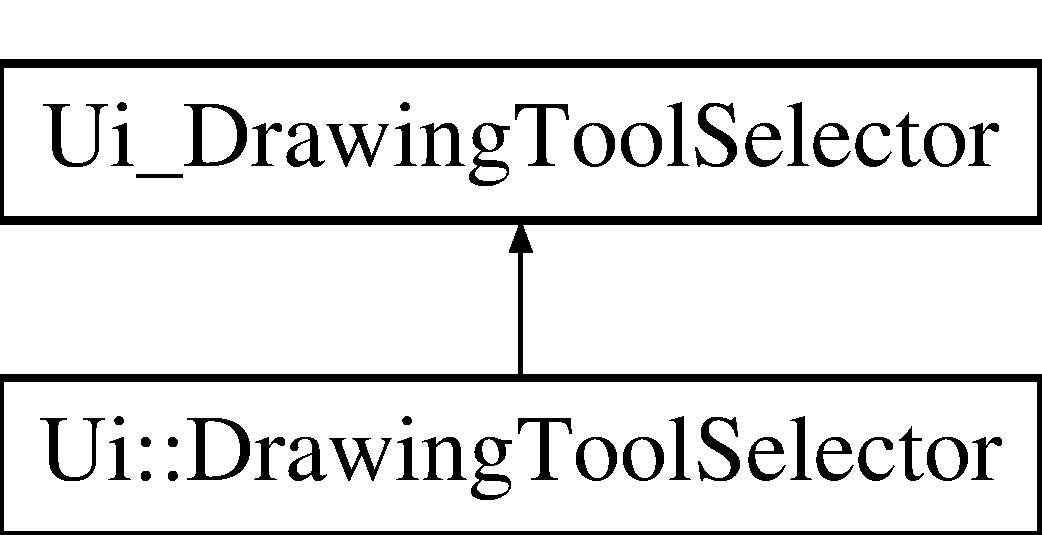
\includegraphics[height=2.000000cm]{class_ui_1_1_drawing_tool_selector}
\end{center}
\end{figure}
\subsection*{Additional Inherited Members}


The documentation for this class was generated from the following file\+:\begin{DoxyCompactItemize}
\item 
\hyperlink{ui__drawingtoolselector_8h}{ui\+\_\+drawingtoolselector.\+h}\end{DoxyCompactItemize}

\hypertarget{class_drawing_tool_selector}{}\section{Drawing\+Tool\+Selector Class Reference}
\label{class_drawing_tool_selector}\index{Drawing\+Tool\+Selector@{Drawing\+Tool\+Selector}}


The \hyperlink{class_drawing_tool_selector}{Drawing\+Tool\+Selector} class.  




{\ttfamily \#include $<$drawingtoolselector.\+h$>$}

Inheritance diagram for Drawing\+Tool\+Selector\+:\begin{figure}[H]
\begin{center}
\leavevmode
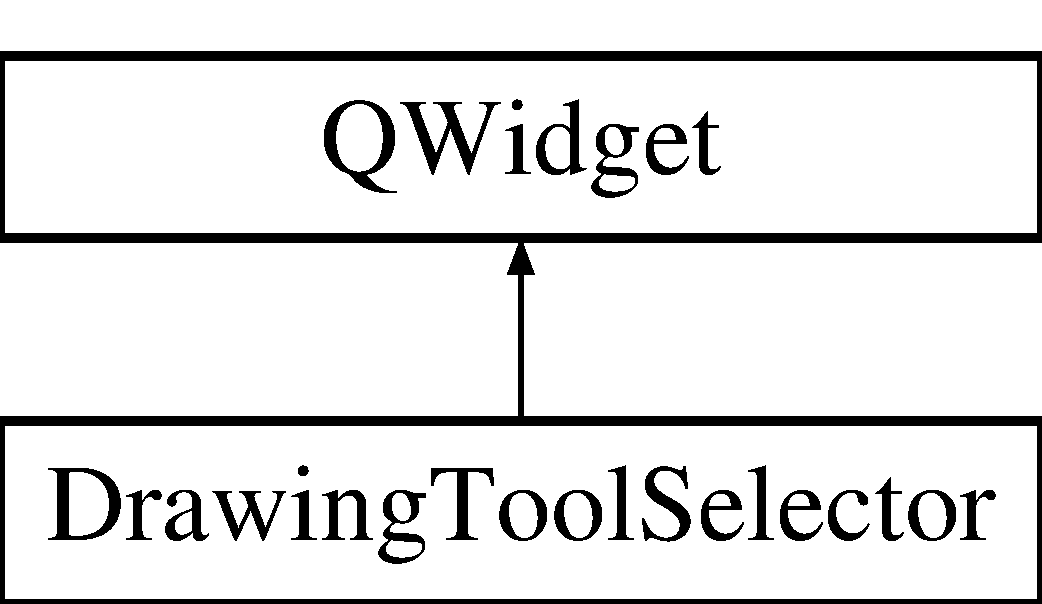
\includegraphics[height=2.000000cm]{class_drawing_tool_selector}
\end{center}
\end{figure}
\subsection*{Public Slots}
\begin{DoxyCompactItemize}
\item 
void \hyperlink{class_drawing_tool_selector_a4d16b789abf92b987ee255c31e887cf0}{set\+Active\+Drawing\+Tool} (const \hyperlink{class_draw_aef97a848de7a634c35c3ce678be88b9b}{Draw\+::\+Tool} \&\hyperlink{class_drawing_tool_selector_a2dd6191c8a1418a2512ae06f43c42a64}{active\+Drawing\+Tool})
\end{DoxyCompactItemize}
\subsection*{Signals}
\begin{DoxyCompactItemize}
\item 
void \hyperlink{class_drawing_tool_selector_a068e4049da8a1155e2070a58d6882b07}{active\+Drawing\+Tool\+Changed} (\hyperlink{class_draw_aef97a848de7a634c35c3ce678be88b9b}{Draw\+::\+Tool} \hyperlink{class_drawing_tool_selector_a2dd6191c8a1418a2512ae06f43c42a64}{active\+Drawing\+Tool})
\end{DoxyCompactItemize}
\subsection*{Public Member Functions}
\begin{DoxyCompactItemize}
\item 
\hyperlink{class_drawing_tool_selector_a04f21c51c1c8eefe90c7974d1551ba7e}{Drawing\+Tool\+Selector} (Q\+Widget $\ast$parent=0)
\item 
\hyperlink{class_drawing_tool_selector_ad5f2e810c40bbeb995711860f6a22394}{$\sim$\+Drawing\+Tool\+Selector} ()
\item 
\hyperlink{class_draw_aef97a848de7a634c35c3ce678be88b9b}{Draw\+::\+Tool} \hyperlink{class_drawing_tool_selector_a2dd6191c8a1418a2512ae06f43c42a64}{active\+Drawing\+Tool} () const
\end{DoxyCompactItemize}
\subsection*{Protected Attributes}
\begin{DoxyCompactItemize}
\item 
\hyperlink{class_draw_aef97a848de7a634c35c3ce678be88b9b}{Draw\+::\+Tool} \hyperlink{class_drawing_tool_selector_ab5f16b690e91d1847f985580accbf79f}{m\+\_\+active\+Drawing\+Tool}
\end{DoxyCompactItemize}


\subsection{Detailed Description}
The \hyperlink{class_drawing_tool_selector}{Drawing\+Tool\+Selector} class. 

\subsection{Constructor \& Destructor Documentation}
\mbox{\Hypertarget{class_drawing_tool_selector_a04f21c51c1c8eefe90c7974d1551ba7e}\label{class_drawing_tool_selector_a04f21c51c1c8eefe90c7974d1551ba7e}} 
\index{Drawing\+Tool\+Selector@{Drawing\+Tool\+Selector}!Drawing\+Tool\+Selector@{Drawing\+Tool\+Selector}}
\index{Drawing\+Tool\+Selector@{Drawing\+Tool\+Selector}!Drawing\+Tool\+Selector@{Drawing\+Tool\+Selector}}
\subsubsection{\texorpdfstring{Drawing\+Tool\+Selector()}{DrawingToolSelector()}}
{\footnotesize\ttfamily Drawing\+Tool\+Selector\+::\+Drawing\+Tool\+Selector (\begin{DoxyParamCaption}\item[{Q\+Widget $\ast$}]{parent = {\ttfamily 0} }\end{DoxyParamCaption})\hspace{0.3cm}{\ttfamily [explicit]}}

\mbox{\Hypertarget{class_drawing_tool_selector_ad5f2e810c40bbeb995711860f6a22394}\label{class_drawing_tool_selector_ad5f2e810c40bbeb995711860f6a22394}} 
\index{Drawing\+Tool\+Selector@{Drawing\+Tool\+Selector}!````~Drawing\+Tool\+Selector@{$\sim$\+Drawing\+Tool\+Selector}}
\index{````~Drawing\+Tool\+Selector@{$\sim$\+Drawing\+Tool\+Selector}!Drawing\+Tool\+Selector@{Drawing\+Tool\+Selector}}
\subsubsection{\texorpdfstring{$\sim$\+Drawing\+Tool\+Selector()}{~DrawingToolSelector()}}
{\footnotesize\ttfamily Drawing\+Tool\+Selector\+::$\sim$\+Drawing\+Tool\+Selector (\begin{DoxyParamCaption}{ }\end{DoxyParamCaption})}



\subsection{Member Function Documentation}
\mbox{\Hypertarget{class_drawing_tool_selector_a2dd6191c8a1418a2512ae06f43c42a64}\label{class_drawing_tool_selector_a2dd6191c8a1418a2512ae06f43c42a64}} 
\index{Drawing\+Tool\+Selector@{Drawing\+Tool\+Selector}!active\+Drawing\+Tool@{active\+Drawing\+Tool}}
\index{active\+Drawing\+Tool@{active\+Drawing\+Tool}!Drawing\+Tool\+Selector@{Drawing\+Tool\+Selector}}
\subsubsection{\texorpdfstring{active\+Drawing\+Tool()}{activeDrawingTool()}}
{\footnotesize\ttfamily \hyperlink{class_draw_aef97a848de7a634c35c3ce678be88b9b}{Draw\+::\+Tool} Drawing\+Tool\+Selector\+::active\+Drawing\+Tool (\begin{DoxyParamCaption}{ }\end{DoxyParamCaption}) const}

\mbox{\Hypertarget{class_drawing_tool_selector_a068e4049da8a1155e2070a58d6882b07}\label{class_drawing_tool_selector_a068e4049da8a1155e2070a58d6882b07}} 
\index{Drawing\+Tool\+Selector@{Drawing\+Tool\+Selector}!active\+Drawing\+Tool\+Changed@{active\+Drawing\+Tool\+Changed}}
\index{active\+Drawing\+Tool\+Changed@{active\+Drawing\+Tool\+Changed}!Drawing\+Tool\+Selector@{Drawing\+Tool\+Selector}}
\subsubsection{\texorpdfstring{active\+Drawing\+Tool\+Changed}{activeDrawingToolChanged}}
{\footnotesize\ttfamily void Drawing\+Tool\+Selector\+::active\+Drawing\+Tool\+Changed (\begin{DoxyParamCaption}\item[{\hyperlink{class_draw_aef97a848de7a634c35c3ce678be88b9b}{Draw\+::\+Tool}}]{active\+Drawing\+Tool }\end{DoxyParamCaption})\hspace{0.3cm}{\ttfamily [signal]}}

\mbox{\Hypertarget{class_drawing_tool_selector_a4d16b789abf92b987ee255c31e887cf0}\label{class_drawing_tool_selector_a4d16b789abf92b987ee255c31e887cf0}} 
\index{Drawing\+Tool\+Selector@{Drawing\+Tool\+Selector}!set\+Active\+Drawing\+Tool@{set\+Active\+Drawing\+Tool}}
\index{set\+Active\+Drawing\+Tool@{set\+Active\+Drawing\+Tool}!Drawing\+Tool\+Selector@{Drawing\+Tool\+Selector}}
\subsubsection{\texorpdfstring{set\+Active\+Drawing\+Tool}{setActiveDrawingTool}}
{\footnotesize\ttfamily void Drawing\+Tool\+Selector\+::set\+Active\+Drawing\+Tool (\begin{DoxyParamCaption}\item[{const \hyperlink{class_draw_aef97a848de7a634c35c3ce678be88b9b}{Draw\+::\+Tool} \&}]{active\+Drawing\+Tool }\end{DoxyParamCaption})\hspace{0.3cm}{\ttfamily [slot]}}



\subsection{Member Data Documentation}
\mbox{\Hypertarget{class_drawing_tool_selector_ab5f16b690e91d1847f985580accbf79f}\label{class_drawing_tool_selector_ab5f16b690e91d1847f985580accbf79f}} 
\index{Drawing\+Tool\+Selector@{Drawing\+Tool\+Selector}!m\+\_\+active\+Drawing\+Tool@{m\+\_\+active\+Drawing\+Tool}}
\index{m\+\_\+active\+Drawing\+Tool@{m\+\_\+active\+Drawing\+Tool}!Drawing\+Tool\+Selector@{Drawing\+Tool\+Selector}}
\subsubsection{\texorpdfstring{m\+\_\+active\+Drawing\+Tool}{m\_activeDrawingTool}}
{\footnotesize\ttfamily \hyperlink{class_draw_aef97a848de7a634c35c3ce678be88b9b}{Draw\+::\+Tool} Drawing\+Tool\+Selector\+::m\+\_\+active\+Drawing\+Tool\hspace{0.3cm}{\ttfamily [protected]}}



The documentation for this class was generated from the following files\+:\begin{DoxyCompactItemize}
\item 
\hyperlink{drawingtoolselector_8h}{drawingtoolselector.\+h}\item 
\hyperlink{drawingtoolselector_8cpp}{drawingtoolselector.\+cpp}\end{DoxyCompactItemize}

\hypertarget{class_graphics_object}{}\section{Graphics\+Object Class Reference}
\label{class_graphics_object}\index{Graphics\+Object@{Graphics\+Object}}


The \hyperlink{class_graphics_object}{Graphics\+Object} class.  




{\ttfamily \#include $<$graphicsobject.\+h$>$}

Inheritance diagram for Graphics\+Object\+:\begin{figure}[H]
\begin{center}
\leavevmode
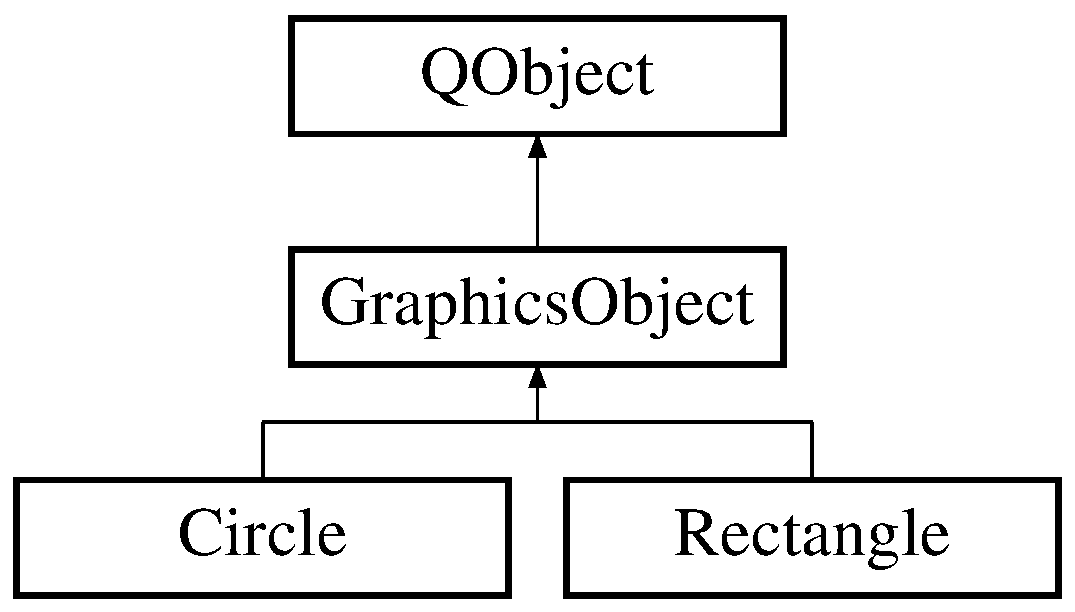
\includegraphics[height=3.000000cm]{class_graphics_object}
\end{center}
\end{figure}
\subsection*{Public Member Functions}
\begin{DoxyCompactItemize}
\item 
\hyperlink{class_graphics_object_a44e1449dabf506461850b88392c26ce2}{Graphics\+Object} (Q\+Object $\ast$parent=0)
\begin{DoxyCompactList}\small\item\em \hyperlink{class_graphics_object_a44e1449dabf506461850b88392c26ce2}{Graphics\+Object\+::\+Graphics\+Object}. \end{DoxyCompactList}\item 
Q\+String \hyperlink{class_graphics_object_ac5591ff2b8009451c593d1197ce7a162}{name} () const
\begin{DoxyCompactList}\small\item\em Getter for name of \hyperlink{class_graphics_object}{Graphics\+Object}. \end{DoxyCompactList}\item 
void \hyperlink{class_graphics_object_a1b0c7c7f87e86833a9a23ab1a2b6f685}{set\+Name} (const Q\+String \&\hyperlink{class_graphics_object_ac5591ff2b8009451c593d1197ce7a162}{name})
\begin{DoxyCompactList}\small\item\em Setter for name of \hyperlink{class_graphics_object}{Graphics\+Object}. \end{DoxyCompactList}\item 
virtual Q\+Graphics\+Item $\ast$ \hyperlink{class_graphics_object_abd625951730f006e748570bf00d158bf}{graphics\+Item} () const
\begin{DoxyCompactList}\small\item\em \hyperlink{class_graphics_object_abd625951730f006e748570bf00d158bf}{Graphics\+Object\+::graphics\+Item}. \end{DoxyCompactList}\item 
qreal \hyperlink{class_graphics_object_a0141eaaf7ab936a2630183c403257026}{posX} () const
\begin{DoxyCompactList}\small\item\em \hyperlink{class_graphics_object_a0141eaaf7ab936a2630183c403257026}{Graphics\+Object\+::posX}. \end{DoxyCompactList}\item 
void \hyperlink{class_graphics_object_ac355db089d870d194e5961921d5626e3}{set\+PosX} (const qreal \&\hyperlink{class_graphics_object_a0141eaaf7ab936a2630183c403257026}{posX})
\begin{DoxyCompactList}\small\item\em \hyperlink{class_graphics_object_ac355db089d870d194e5961921d5626e3}{Graphics\+Object\+::set\+PosX}. \end{DoxyCompactList}\item 
qreal \hyperlink{class_graphics_object_adfd441f0d80339456482cc71355ba429}{posY} () const
\begin{DoxyCompactList}\small\item\em \hyperlink{class_graphics_object_adfd441f0d80339456482cc71355ba429}{Graphics\+Object\+::posY}. \end{DoxyCompactList}\item 
void \hyperlink{class_graphics_object_ab450d85cfafd5eb80c2ce75784e13088}{set\+PosY} (const qreal \&\hyperlink{class_graphics_object_adfd441f0d80339456482cc71355ba429}{posY})
\begin{DoxyCompactList}\small\item\em \hyperlink{class_graphics_object_ab450d85cfafd5eb80c2ce75784e13088}{Graphics\+Object\+::set\+PosY}. \end{DoxyCompactList}\item 
Q\+Color \hyperlink{class_graphics_object_a2d1ae6917ba3a02c305ce48f04e4aa65}{border\+Color} () const
\begin{DoxyCompactList}\small\item\em \hyperlink{class_graphics_object_a2d1ae6917ba3a02c305ce48f04e4aa65}{Graphics\+Object\+::border\+Color}. \end{DoxyCompactList}\item 
void \hyperlink{class_graphics_object_a23b8350a123074dfcd5b3807bda06487}{set\+Border\+Color} (const Q\+Color \&\hyperlink{class_graphics_object_a2d1ae6917ba3a02c305ce48f04e4aa65}{border\+Color})
\begin{DoxyCompactList}\small\item\em \hyperlink{class_graphics_object_a23b8350a123074dfcd5b3807bda06487}{Graphics\+Object\+::set\+Border\+Color}. \end{DoxyCompactList}\item 
Q\+Color \hyperlink{class_graphics_object_a2575009e9051dc8cd582c23ceb4cebec}{fill\+Color} () const
\begin{DoxyCompactList}\small\item\em \hyperlink{class_graphics_object_a2575009e9051dc8cd582c23ceb4cebec}{Graphics\+Object\+::fill\+Color}. \end{DoxyCompactList}\item 
void \hyperlink{class_graphics_object_a125ba24bcb7f858a20054a9c57ae8a97}{set\+Fill\+Color} (const Q\+Color \&\hyperlink{class_graphics_object_a2575009e9051dc8cd582c23ceb4cebec}{fill\+Color})
\begin{DoxyCompactList}\small\item\em \hyperlink{class_graphics_object_a125ba24bcb7f858a20054a9c57ae8a97}{Graphics\+Object\+::set\+Fill\+Color}. \end{DoxyCompactList}\end{DoxyCompactItemize}


\subsection{Detailed Description}
The \hyperlink{class_graphics_object}{Graphics\+Object} class. 

\subsection{Constructor \& Destructor Documentation}
\mbox{\Hypertarget{class_graphics_object_a44e1449dabf506461850b88392c26ce2}\label{class_graphics_object_a44e1449dabf506461850b88392c26ce2}} 
\index{Graphics\+Object@{Graphics\+Object}!Graphics\+Object@{Graphics\+Object}}
\index{Graphics\+Object@{Graphics\+Object}!Graphics\+Object@{Graphics\+Object}}
\subsubsection{\texorpdfstring{Graphics\+Object()}{GraphicsObject()}}
{\footnotesize\ttfamily Graphics\+Object\+::\+Graphics\+Object (\begin{DoxyParamCaption}\item[{Q\+Object $\ast$}]{parent = {\ttfamily 0} }\end{DoxyParamCaption})\hspace{0.3cm}{\ttfamily [explicit]}}



\hyperlink{class_graphics_object_a44e1449dabf506461850b88392c26ce2}{Graphics\+Object\+::\+Graphics\+Object}. 


\begin{DoxyParams}{Parameters}
{\em parent} & is 0 \\
\hline
\end{DoxyParams}


\subsection{Member Function Documentation}
\mbox{\Hypertarget{class_graphics_object_a2d1ae6917ba3a02c305ce48f04e4aa65}\label{class_graphics_object_a2d1ae6917ba3a02c305ce48f04e4aa65}} 
\index{Graphics\+Object@{Graphics\+Object}!border\+Color@{border\+Color}}
\index{border\+Color@{border\+Color}!Graphics\+Object@{Graphics\+Object}}
\subsubsection{\texorpdfstring{border\+Color()}{borderColor()}}
{\footnotesize\ttfamily Q\+Color Graphics\+Object\+::border\+Color (\begin{DoxyParamCaption}{ }\end{DoxyParamCaption}) const}



\hyperlink{class_graphics_object_a2d1ae6917ba3a02c305ce48f04e4aa65}{Graphics\+Object\+::border\+Color}. 

\begin{DoxyReturn}{Returns}

\end{DoxyReturn}
\mbox{\Hypertarget{class_graphics_object_a2575009e9051dc8cd582c23ceb4cebec}\label{class_graphics_object_a2575009e9051dc8cd582c23ceb4cebec}} 
\index{Graphics\+Object@{Graphics\+Object}!fill\+Color@{fill\+Color}}
\index{fill\+Color@{fill\+Color}!Graphics\+Object@{Graphics\+Object}}
\subsubsection{\texorpdfstring{fill\+Color()}{fillColor()}}
{\footnotesize\ttfamily Q\+Color Graphics\+Object\+::fill\+Color (\begin{DoxyParamCaption}{ }\end{DoxyParamCaption}) const}



\hyperlink{class_graphics_object_a2575009e9051dc8cd582c23ceb4cebec}{Graphics\+Object\+::fill\+Color}. 

\begin{DoxyReturn}{Returns}

\end{DoxyReturn}
\mbox{\Hypertarget{class_graphics_object_abd625951730f006e748570bf00d158bf}\label{class_graphics_object_abd625951730f006e748570bf00d158bf}} 
\index{Graphics\+Object@{Graphics\+Object}!graphics\+Item@{graphics\+Item}}
\index{graphics\+Item@{graphics\+Item}!Graphics\+Object@{Graphics\+Object}}
\subsubsection{\texorpdfstring{graphics\+Item()}{graphicsItem()}}
{\footnotesize\ttfamily Q\+Graphics\+Item $\ast$ Graphics\+Object\+::graphics\+Item (\begin{DoxyParamCaption}{ }\end{DoxyParamCaption}) const\hspace{0.3cm}{\ttfamily [virtual]}}



\hyperlink{class_graphics_object_abd625951730f006e748570bf00d158bf}{Graphics\+Object\+::graphics\+Item}. 

\begin{DoxyReturn}{Returns}

\end{DoxyReturn}


Reimplemented in \hyperlink{class_rectangle_a6d2cdec338bb43ad533b98e58eea9e03}{Rectangle}, and \hyperlink{class_circle_ad1fa0a922709e61b3e70eef604a3600d}{Circle}.

\mbox{\Hypertarget{class_graphics_object_ac5591ff2b8009451c593d1197ce7a162}\label{class_graphics_object_ac5591ff2b8009451c593d1197ce7a162}} 
\index{Graphics\+Object@{Graphics\+Object}!name@{name}}
\index{name@{name}!Graphics\+Object@{Graphics\+Object}}
\subsubsection{\texorpdfstring{name()}{name()}}
{\footnotesize\ttfamily Q\+String Graphics\+Object\+::name (\begin{DoxyParamCaption}{ }\end{DoxyParamCaption}) const}



Getter for name of \hyperlink{class_graphics_object}{Graphics\+Object}. 

\begin{DoxyReturn}{Returns}
m\+\_\+name 
\end{DoxyReturn}
\mbox{\Hypertarget{class_graphics_object_a0141eaaf7ab936a2630183c403257026}\label{class_graphics_object_a0141eaaf7ab936a2630183c403257026}} 
\index{Graphics\+Object@{Graphics\+Object}!posX@{posX}}
\index{posX@{posX}!Graphics\+Object@{Graphics\+Object}}
\subsubsection{\texorpdfstring{pos\+X()}{posX()}}
{\footnotesize\ttfamily qreal Graphics\+Object\+::posX (\begin{DoxyParamCaption}{ }\end{DoxyParamCaption}) const}



\hyperlink{class_graphics_object_a0141eaaf7ab936a2630183c403257026}{Graphics\+Object\+::posX}. 

\begin{DoxyReturn}{Returns}

\end{DoxyReturn}
\mbox{\Hypertarget{class_graphics_object_adfd441f0d80339456482cc71355ba429}\label{class_graphics_object_adfd441f0d80339456482cc71355ba429}} 
\index{Graphics\+Object@{Graphics\+Object}!posY@{posY}}
\index{posY@{posY}!Graphics\+Object@{Graphics\+Object}}
\subsubsection{\texorpdfstring{pos\+Y()}{posY()}}
{\footnotesize\ttfamily qreal Graphics\+Object\+::posY (\begin{DoxyParamCaption}{ }\end{DoxyParamCaption}) const}



\hyperlink{class_graphics_object_adfd441f0d80339456482cc71355ba429}{Graphics\+Object\+::posY}. 

\begin{DoxyReturn}{Returns}

\end{DoxyReturn}
\mbox{\Hypertarget{class_graphics_object_a23b8350a123074dfcd5b3807bda06487}\label{class_graphics_object_a23b8350a123074dfcd5b3807bda06487}} 
\index{Graphics\+Object@{Graphics\+Object}!set\+Border\+Color@{set\+Border\+Color}}
\index{set\+Border\+Color@{set\+Border\+Color}!Graphics\+Object@{Graphics\+Object}}
\subsubsection{\texorpdfstring{set\+Border\+Color()}{setBorderColor()}}
{\footnotesize\ttfamily void Graphics\+Object\+::set\+Border\+Color (\begin{DoxyParamCaption}\item[{const Q\+Color \&}]{border\+Color }\end{DoxyParamCaption})}



\hyperlink{class_graphics_object_a23b8350a123074dfcd5b3807bda06487}{Graphics\+Object\+::set\+Border\+Color}. 


\begin{DoxyParams}{Parameters}
{\em border\+Color} & \\
\hline
\end{DoxyParams}
\mbox{\Hypertarget{class_graphics_object_a125ba24bcb7f858a20054a9c57ae8a97}\label{class_graphics_object_a125ba24bcb7f858a20054a9c57ae8a97}} 
\index{Graphics\+Object@{Graphics\+Object}!set\+Fill\+Color@{set\+Fill\+Color}}
\index{set\+Fill\+Color@{set\+Fill\+Color}!Graphics\+Object@{Graphics\+Object}}
\subsubsection{\texorpdfstring{set\+Fill\+Color()}{setFillColor()}}
{\footnotesize\ttfamily void Graphics\+Object\+::set\+Fill\+Color (\begin{DoxyParamCaption}\item[{const Q\+Color \&}]{fill\+Color }\end{DoxyParamCaption})}



\hyperlink{class_graphics_object_a125ba24bcb7f858a20054a9c57ae8a97}{Graphics\+Object\+::set\+Fill\+Color}. 


\begin{DoxyParams}{Parameters}
{\em fill\+Color} & \\
\hline
\end{DoxyParams}
\mbox{\Hypertarget{class_graphics_object_a1b0c7c7f87e86833a9a23ab1a2b6f685}\label{class_graphics_object_a1b0c7c7f87e86833a9a23ab1a2b6f685}} 
\index{Graphics\+Object@{Graphics\+Object}!set\+Name@{set\+Name}}
\index{set\+Name@{set\+Name}!Graphics\+Object@{Graphics\+Object}}
\subsubsection{\texorpdfstring{set\+Name()}{setName()}}
{\footnotesize\ttfamily void Graphics\+Object\+::set\+Name (\begin{DoxyParamCaption}\item[{const Q\+String \&}]{name }\end{DoxyParamCaption})}



Setter for name of \hyperlink{class_graphics_object}{Graphics\+Object}. 


\begin{DoxyParams}{Parameters}
{\em new} & name \\
\hline
\end{DoxyParams}
\mbox{\Hypertarget{class_graphics_object_ac355db089d870d194e5961921d5626e3}\label{class_graphics_object_ac355db089d870d194e5961921d5626e3}} 
\index{Graphics\+Object@{Graphics\+Object}!set\+PosX@{set\+PosX}}
\index{set\+PosX@{set\+PosX}!Graphics\+Object@{Graphics\+Object}}
\subsubsection{\texorpdfstring{set\+Pos\+X()}{setPosX()}}
{\footnotesize\ttfamily void Graphics\+Object\+::set\+PosX (\begin{DoxyParamCaption}\item[{const qreal \&}]{posX }\end{DoxyParamCaption})}



\hyperlink{class_graphics_object_ac355db089d870d194e5961921d5626e3}{Graphics\+Object\+::set\+PosX}. 


\begin{DoxyParams}{Parameters}
{\em posX} & \\
\hline
\end{DoxyParams}
\mbox{\Hypertarget{class_graphics_object_ab450d85cfafd5eb80c2ce75784e13088}\label{class_graphics_object_ab450d85cfafd5eb80c2ce75784e13088}} 
\index{Graphics\+Object@{Graphics\+Object}!set\+PosY@{set\+PosY}}
\index{set\+PosY@{set\+PosY}!Graphics\+Object@{Graphics\+Object}}
\subsubsection{\texorpdfstring{set\+Pos\+Y()}{setPosY()}}
{\footnotesize\ttfamily void Graphics\+Object\+::set\+PosY (\begin{DoxyParamCaption}\item[{const qreal \&}]{posY }\end{DoxyParamCaption})}



\hyperlink{class_graphics_object_ab450d85cfafd5eb80c2ce75784e13088}{Graphics\+Object\+::set\+PosY}. 


\begin{DoxyParams}{Parameters}
{\em posY} & \\
\hline
\end{DoxyParams}


The documentation for this class was generated from the following files\+:\begin{DoxyCompactItemize}
\item 
\hyperlink{graphicsobject_8h}{graphicsobject.\+h}\item 
\hyperlink{graphicsobject_8cpp}{graphicsobject.\+cpp}\end{DoxyCompactItemize}

\hypertarget{class_graphics_object_map}{}\section{Graphics\+Object\+Map Class Reference}
\label{class_graphics_object_map}\index{Graphics\+Object\+Map@{Graphics\+Object\+Map}}


{\ttfamily \#include $<$graphicsobjectmap.\+h$>$}

Inheritance diagram for Graphics\+Object\+Map\+:\begin{figure}[H]
\begin{center}
\leavevmode
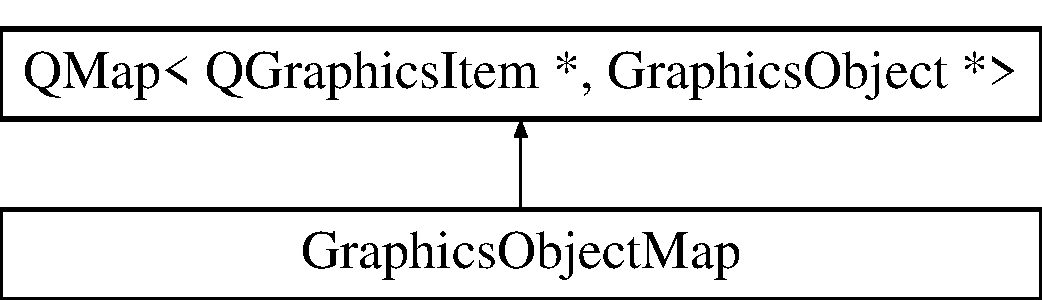
\includegraphics[height=2.000000cm]{class_graphics_object_map}
\end{center}
\end{figure}
\subsection*{Public Member Functions}
\begin{DoxyCompactItemize}
\item 
\hyperlink{class_graphics_object_map_a31e38788b129d655fa53e26d489cbf8c}{Graphics\+Object\+Map} ()
\item 
void \hyperlink{class_graphics_object_map_a5e9632b78470d797613114dae0382028}{Print\+Objects} ()
\begin{DoxyCompactList}\small\item\em Prints all objects of map object. \end{DoxyCompactList}\end{DoxyCompactItemize}
\subsection*{Public Attributes}
\begin{DoxyCompactItemize}
\item 
Q\+Map$<$ Q\+Graphics\+Item $\ast$, \hyperlink{class_graphics_object}{Graphics\+Object} $\ast$ $>$ \hyperlink{class_graphics_object_map_a6b59cd95bfc0fcbec8037e12edc7a3e1}{my\+Map}
\end{DoxyCompactItemize}


\subsection{Constructor \& Destructor Documentation}
\mbox{\Hypertarget{class_graphics_object_map_a31e38788b129d655fa53e26d489cbf8c}\label{class_graphics_object_map_a31e38788b129d655fa53e26d489cbf8c}} 
\index{Graphics\+Object\+Map@{Graphics\+Object\+Map}!Graphics\+Object\+Map@{Graphics\+Object\+Map}}
\index{Graphics\+Object\+Map@{Graphics\+Object\+Map}!Graphics\+Object\+Map@{Graphics\+Object\+Map}}
\subsubsection{\texorpdfstring{Graphics\+Object\+Map()}{GraphicsObjectMap()}}
{\footnotesize\ttfamily Graphics\+Object\+Map\+::\+Graphics\+Object\+Map (\begin{DoxyParamCaption}{ }\end{DoxyParamCaption})}



\subsection{Member Function Documentation}
\mbox{\Hypertarget{class_graphics_object_map_a5e9632b78470d797613114dae0382028}\label{class_graphics_object_map_a5e9632b78470d797613114dae0382028}} 
\index{Graphics\+Object\+Map@{Graphics\+Object\+Map}!Print\+Objects@{Print\+Objects}}
\index{Print\+Objects@{Print\+Objects}!Graphics\+Object\+Map@{Graphics\+Object\+Map}}
\subsubsection{\texorpdfstring{Print\+Objects()}{PrintObjects()}}
{\footnotesize\ttfamily void Graphics\+Object\+Map\+::\+Print\+Objects (\begin{DoxyParamCaption}{ }\end{DoxyParamCaption})}



Prints all objects of map object. 



\subsection{Member Data Documentation}
\mbox{\Hypertarget{class_graphics_object_map_a6b59cd95bfc0fcbec8037e12edc7a3e1}\label{class_graphics_object_map_a6b59cd95bfc0fcbec8037e12edc7a3e1}} 
\index{Graphics\+Object\+Map@{Graphics\+Object\+Map}!my\+Map@{my\+Map}}
\index{my\+Map@{my\+Map}!Graphics\+Object\+Map@{Graphics\+Object\+Map}}
\subsubsection{\texorpdfstring{my\+Map}{myMap}}
{\footnotesize\ttfamily Q\+Map$<$Q\+Graphics\+Item $\ast$, \hyperlink{class_graphics_object}{Graphics\+Object} $\ast$$>$ Graphics\+Object\+Map\+::my\+Map}



The documentation for this class was generated from the following files\+:\begin{DoxyCompactItemize}
\item 
\hyperlink{graphicsobjectmap_8h}{graphicsobjectmap.\+h}\item 
\hyperlink{graphicsobjectmap_8cpp}{graphicsobjectmap.\+cpp}\end{DoxyCompactItemize}

\hypertarget{class_graphics_scene}{}\section{Graphics\+Scene Class Reference}
\label{class_graphics_scene}\index{Graphics\+Scene@{Graphics\+Scene}}


The \hyperlink{class_graphics_scene}{Graphics\+Scene} class.  




{\ttfamily \#include $<$graphicsscene.\+h$>$}

Inheritance diagram for Graphics\+Scene\+:\begin{figure}[H]
\begin{center}
\leavevmode
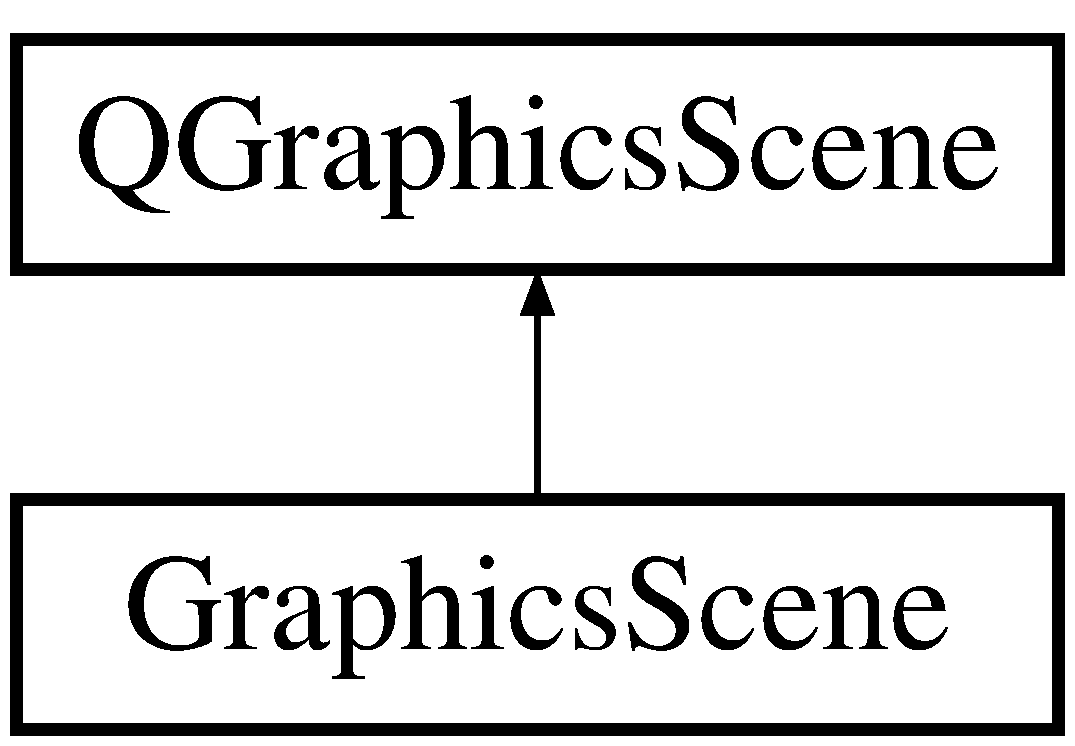
\includegraphics[height=2.000000cm]{class_graphics_scene}
\end{center}
\end{figure}
\subsection*{Public Slots}
\begin{DoxyCompactItemize}
\item 
void \hyperlink{class_graphics_scene_a99831b8b30259a344715f95d65427465}{set\+Active\+Drawing\+Tool} (const \hyperlink{class_draw_aef97a848de7a634c35c3ce678be88b9b}{Draw\+::\+Tool} \&active\+Drawing\+Tool)
\item 
void \hyperlink{class_graphics_scene_a48f32ef7c39d728cc7c7eb9d21dbffca}{set\+Current\+Map} (\hyperlink{class_graphics_object_map}{Graphics\+Object\+Map} object\+Map)
\end{DoxyCompactItemize}
\subsection*{Signals}
\begin{DoxyCompactItemize}
\item 
void \hyperlink{class_graphics_scene_acfc07dfc3d559fc497cde524dc8ffa66}{new\+Point\+Selected} (Q\+PointF new\+Point)
\end{DoxyCompactItemize}
\subsection*{Public Member Functions}
\begin{DoxyCompactItemize}
\item 
\hyperlink{class_graphics_scene_a8e12dad680e5944c7ecce5b399595742}{Graphics\+Scene} (Q\+Object $\ast$parent=0)
\begin{DoxyCompactList}\small\item\em \hyperlink{class_graphics_scene_a8e12dad680e5944c7ecce5b399595742}{Graphics\+Scene\+::\+Graphics\+Scene}. \end{DoxyCompactList}\item 
\hyperlink{class_graphics_scene_a49bf5569f93aa92ecf99c89c14a0b17d}{$\sim$\+Graphics\+Scene} ()
\item 
Q\+PointF \hyperlink{class_graphics_scene_aa341f24da86296d2f06fe485857b54b5}{get\+My\+Point} () const
\item 
void \hyperlink{class_graphics_scene_a2853f7e6ab37aeaa25c1dfc2d33eb7af}{set\+My\+Point} (const Q\+PointF \&value)
\item 
void \hyperlink{class_graphics_scene_aa6c883ed523812e7aec5018888b72ee1}{create\+Grid} ()
\begin{DoxyCompactList}\small\item\em \hyperlink{class_graphics_scene_aa6c883ed523812e7aec5018888b72ee1}{Graphics\+Scene\+::create\+Grid}. \end{DoxyCompactList}\item 
void \hyperlink{class_graphics_scene_ae2cdfb607a8ce680f0ed8c93c519ff01}{mouse\+Press\+Event} (Q\+Graphics\+Scene\+Mouse\+Event $\ast$mouse\+Event) override
\item 
void \hyperlink{class_graphics_scene_a1bc5a1a813d1ff00bba4e919ed1b7525}{mouse\+Move\+Event} (Q\+Graphics\+Scene\+Mouse\+Event $\ast$mouse\+Event) override
\begin{DoxyCompactList}\small\item\em \hyperlink{class_graphics_scene_a1bc5a1a813d1ff00bba4e919ed1b7525}{Graphics\+Scene\+::mouse\+Move\+Event}. \end{DoxyCompactList}\item 
void \hyperlink{class_graphics_scene_a5f83aea5c35bad170a3c766ab41bacf5}{mouse\+Release\+Event} (Q\+Graphics\+Scene\+Mouse\+Event $\ast$mouse\+Event) override
\end{DoxyCompactItemize}


\subsection{Detailed Description}
The \hyperlink{class_graphics_scene}{Graphics\+Scene} class. 

\subsection{Constructor \& Destructor Documentation}
\mbox{\Hypertarget{class_graphics_scene_a8e12dad680e5944c7ecce5b399595742}\label{class_graphics_scene_a8e12dad680e5944c7ecce5b399595742}} 
\index{Graphics\+Scene@{Graphics\+Scene}!Graphics\+Scene@{Graphics\+Scene}}
\index{Graphics\+Scene@{Graphics\+Scene}!Graphics\+Scene@{Graphics\+Scene}}
\subsubsection{\texorpdfstring{Graphics\+Scene()}{GraphicsScene()}}
{\footnotesize\ttfamily Graphics\+Scene\+::\+Graphics\+Scene (\begin{DoxyParamCaption}\item[{Q\+Object $\ast$}]{parent = {\ttfamily 0} }\end{DoxyParamCaption})\hspace{0.3cm}{\ttfamily [explicit]}}



\hyperlink{class_graphics_scene_a8e12dad680e5944c7ecce5b399595742}{Graphics\+Scene\+::\+Graphics\+Scene}. 


\begin{DoxyParams}{Parameters}
{\em parent} & \\
\hline
\end{DoxyParams}
\begin{DoxyParagraph}{Graphics\+Scene}
The \hyperlink{class_graphics_scene}{Graphics\+Scene} class manages the user interaction 
\end{DoxyParagraph}
\mbox{\Hypertarget{class_graphics_scene_a49bf5569f93aa92ecf99c89c14a0b17d}\label{class_graphics_scene_a49bf5569f93aa92ecf99c89c14a0b17d}} 
\index{Graphics\+Scene@{Graphics\+Scene}!````~Graphics\+Scene@{$\sim$\+Graphics\+Scene}}
\index{````~Graphics\+Scene@{$\sim$\+Graphics\+Scene}!Graphics\+Scene@{Graphics\+Scene}}
\subsubsection{\texorpdfstring{$\sim$\+Graphics\+Scene()}{~GraphicsScene()}}
{\footnotesize\ttfamily Graphics\+Scene\+::$\sim$\+Graphics\+Scene (\begin{DoxyParamCaption}{ }\end{DoxyParamCaption})}



\subsection{Member Function Documentation}
\mbox{\Hypertarget{class_graphics_scene_aa6c883ed523812e7aec5018888b72ee1}\label{class_graphics_scene_aa6c883ed523812e7aec5018888b72ee1}} 
\index{Graphics\+Scene@{Graphics\+Scene}!create\+Grid@{create\+Grid}}
\index{create\+Grid@{create\+Grid}!Graphics\+Scene@{Graphics\+Scene}}
\subsubsection{\texorpdfstring{create\+Grid()}{createGrid()}}
{\footnotesize\ttfamily void Graphics\+Scene\+::create\+Grid (\begin{DoxyParamCaption}{ }\end{DoxyParamCaption})}



\hyperlink{class_graphics_scene_aa6c883ed523812e7aec5018888b72ee1}{Graphics\+Scene\+::create\+Grid}. 

\begin{DoxyParagraph}{The grid}
Generates the grid to mark the units 
\end{DoxyParagraph}
\mbox{\Hypertarget{class_graphics_scene_aa341f24da86296d2f06fe485857b54b5}\label{class_graphics_scene_aa341f24da86296d2f06fe485857b54b5}} 
\index{Graphics\+Scene@{Graphics\+Scene}!get\+My\+Point@{get\+My\+Point}}
\index{get\+My\+Point@{get\+My\+Point}!Graphics\+Scene@{Graphics\+Scene}}
\subsubsection{\texorpdfstring{get\+My\+Point()}{getMyPoint()}}
{\footnotesize\ttfamily Q\+PointF Graphics\+Scene\+::get\+My\+Point (\begin{DoxyParamCaption}{ }\end{DoxyParamCaption}) const}

\mbox{\Hypertarget{class_graphics_scene_a1bc5a1a813d1ff00bba4e919ed1b7525}\label{class_graphics_scene_a1bc5a1a813d1ff00bba4e919ed1b7525}} 
\index{Graphics\+Scene@{Graphics\+Scene}!mouse\+Move\+Event@{mouse\+Move\+Event}}
\index{mouse\+Move\+Event@{mouse\+Move\+Event}!Graphics\+Scene@{Graphics\+Scene}}
\subsubsection{\texorpdfstring{mouse\+Move\+Event()}{mouseMoveEvent()}}
{\footnotesize\ttfamily void Graphics\+Scene\+::mouse\+Move\+Event (\begin{DoxyParamCaption}\item[{Q\+Graphics\+Scene\+Mouse\+Event $\ast$}]{mouse\+Event }\end{DoxyParamCaption})\hspace{0.3cm}{\ttfamily [override]}}



\hyperlink{class_graphics_scene_a1bc5a1a813d1ff00bba4e919ed1b7525}{Graphics\+Scene\+::mouse\+Move\+Event}. 


\begin{DoxyParams}{Parameters}
{\em mouse\+Event} & \\
\hline
\end{DoxyParams}
\begin{DoxyParagraph}{Move}
This function moves the items when pressed and shows names on hover 
\end{DoxyParagraph}
\mbox{\Hypertarget{class_graphics_scene_ae2cdfb607a8ce680f0ed8c93c519ff01}\label{class_graphics_scene_ae2cdfb607a8ce680f0ed8c93c519ff01}} 
\index{Graphics\+Scene@{Graphics\+Scene}!mouse\+Press\+Event@{mouse\+Press\+Event}}
\index{mouse\+Press\+Event@{mouse\+Press\+Event}!Graphics\+Scene@{Graphics\+Scene}}
\subsubsection{\texorpdfstring{mouse\+Press\+Event()}{mousePressEvent()}}
{\footnotesize\ttfamily void Graphics\+Scene\+::mouse\+Press\+Event (\begin{DoxyParamCaption}\item[{Q\+Graphics\+Scene\+Mouse\+Event $\ast$}]{mouse\+Event }\end{DoxyParamCaption})\hspace{0.3cm}{\ttfamily [override]}}

\mbox{\Hypertarget{class_graphics_scene_a5f83aea5c35bad170a3c766ab41bacf5}\label{class_graphics_scene_a5f83aea5c35bad170a3c766ab41bacf5}} 
\index{Graphics\+Scene@{Graphics\+Scene}!mouse\+Release\+Event@{mouse\+Release\+Event}}
\index{mouse\+Release\+Event@{mouse\+Release\+Event}!Graphics\+Scene@{Graphics\+Scene}}
\subsubsection{\texorpdfstring{mouse\+Release\+Event()}{mouseReleaseEvent()}}
{\footnotesize\ttfamily void Graphics\+Scene\+::mouse\+Release\+Event (\begin{DoxyParamCaption}\item[{Q\+Graphics\+Scene\+Mouse\+Event $\ast$}]{mouse\+Event }\end{DoxyParamCaption})\hspace{0.3cm}{\ttfamily [override]}}

\mbox{\Hypertarget{class_graphics_scene_acfc07dfc3d559fc497cde524dc8ffa66}\label{class_graphics_scene_acfc07dfc3d559fc497cde524dc8ffa66}} 
\index{Graphics\+Scene@{Graphics\+Scene}!new\+Point\+Selected@{new\+Point\+Selected}}
\index{new\+Point\+Selected@{new\+Point\+Selected}!Graphics\+Scene@{Graphics\+Scene}}
\subsubsection{\texorpdfstring{new\+Point\+Selected}{newPointSelected}}
{\footnotesize\ttfamily void Graphics\+Scene\+::new\+Point\+Selected (\begin{DoxyParamCaption}\item[{Q\+PointF}]{new\+Point }\end{DoxyParamCaption})\hspace{0.3cm}{\ttfamily [signal]}}

\mbox{\Hypertarget{class_graphics_scene_a99831b8b30259a344715f95d65427465}\label{class_graphics_scene_a99831b8b30259a344715f95d65427465}} 
\index{Graphics\+Scene@{Graphics\+Scene}!set\+Active\+Drawing\+Tool@{set\+Active\+Drawing\+Tool}}
\index{set\+Active\+Drawing\+Tool@{set\+Active\+Drawing\+Tool}!Graphics\+Scene@{Graphics\+Scene}}
\subsubsection{\texorpdfstring{set\+Active\+Drawing\+Tool}{setActiveDrawingTool}}
{\footnotesize\ttfamily void Graphics\+Scene\+::set\+Active\+Drawing\+Tool (\begin{DoxyParamCaption}\item[{const \hyperlink{class_draw_aef97a848de7a634c35c3ce678be88b9b}{Draw\+::\+Tool} \&}]{active\+Drawing\+Tool }\end{DoxyParamCaption})\hspace{0.3cm}{\ttfamily [slot]}}

\mbox{\Hypertarget{class_graphics_scene_a48f32ef7c39d728cc7c7eb9d21dbffca}\label{class_graphics_scene_a48f32ef7c39d728cc7c7eb9d21dbffca}} 
\index{Graphics\+Scene@{Graphics\+Scene}!set\+Current\+Map@{set\+Current\+Map}}
\index{set\+Current\+Map@{set\+Current\+Map}!Graphics\+Scene@{Graphics\+Scene}}
\subsubsection{\texorpdfstring{set\+Current\+Map}{setCurrentMap}}
{\footnotesize\ttfamily void Graphics\+Scene\+::set\+Current\+Map (\begin{DoxyParamCaption}\item[{\hyperlink{class_graphics_object_map}{Graphics\+Object\+Map}}]{object\+Map }\end{DoxyParamCaption})\hspace{0.3cm}{\ttfamily [slot]}}

\mbox{\Hypertarget{class_graphics_scene_a2853f7e6ab37aeaa25c1dfc2d33eb7af}\label{class_graphics_scene_a2853f7e6ab37aeaa25c1dfc2d33eb7af}} 
\index{Graphics\+Scene@{Graphics\+Scene}!set\+My\+Point@{set\+My\+Point}}
\index{set\+My\+Point@{set\+My\+Point}!Graphics\+Scene@{Graphics\+Scene}}
\subsubsection{\texorpdfstring{set\+My\+Point()}{setMyPoint()}}
{\footnotesize\ttfamily void Graphics\+Scene\+::set\+My\+Point (\begin{DoxyParamCaption}\item[{const Q\+PointF \&}]{value }\end{DoxyParamCaption})}



The documentation for this class was generated from the following files\+:\begin{DoxyCompactItemize}
\item 
\hyperlink{graphicsscene_8h}{graphicsscene.\+h}\item 
\hyperlink{graphicsscene_8cpp}{graphicsscene.\+cpp}\end{DoxyCompactItemize}

\hypertarget{class_main_window}{}\section{Main\+Window Class Reference}
\label{class_main_window}\index{Main\+Window@{Main\+Window}}


{\ttfamily \#include $<$mainwindow.\+h$>$}

Inheritance diagram for Main\+Window\+:\begin{figure}[H]
\begin{center}
\leavevmode
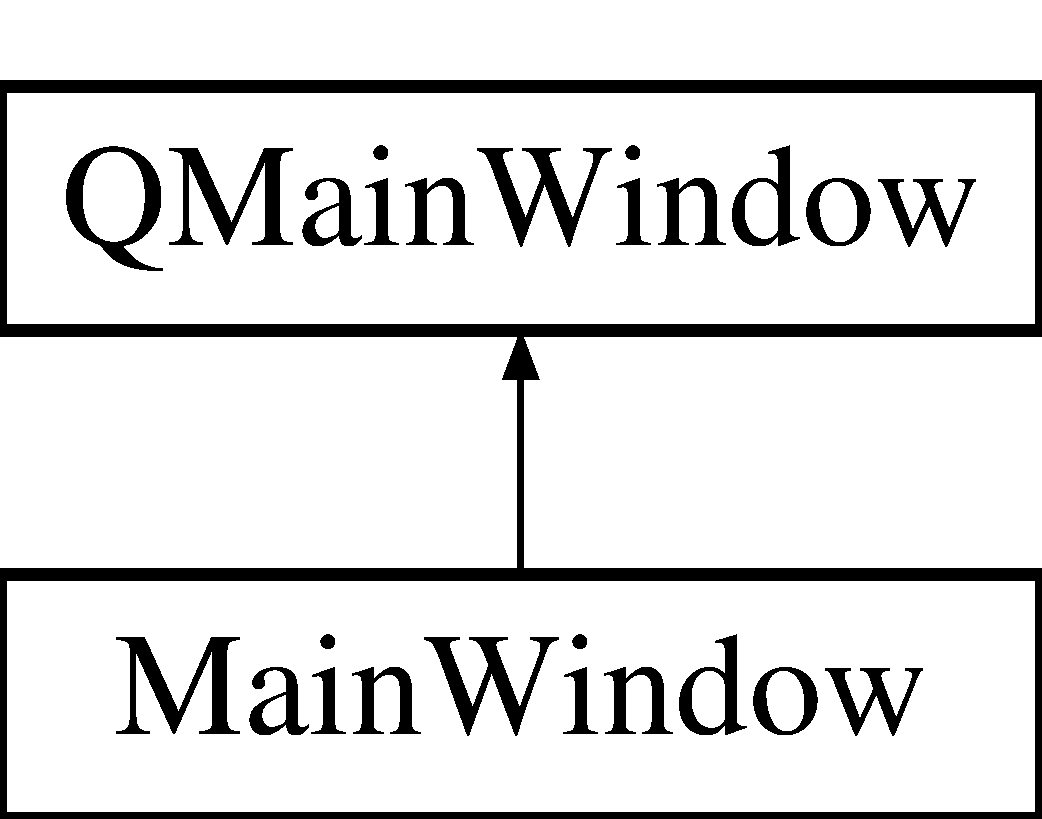
\includegraphics[height=2.000000cm]{class_main_window}
\end{center}
\end{figure}
\subsection*{Public Slots}
\begin{DoxyCompactItemize}
\item 
void \hyperlink{class_main_window_a91d63c0ae1ebabef78c51f976b763deb}{generate\+New\+UI} (\hyperlink{class_draw_aef97a848de7a634c35c3ce678be88b9b}{Draw\+::\+Tool} selected\+Tool)
\begin{DoxyCompactList}\small\item\em Manipulates UI. \end{DoxyCompactList}\item 
void \hyperlink{class_main_window_ae60e9e64c47018bff59b20337b688936}{set\+Active\+Drawing\+Tool} (\hyperlink{class_draw_aef97a848de7a634c35c3ce678be88b9b}{Draw\+::\+Tool} active\+Drawing\+Tool)
\begin{DoxyCompactList}\small\item\em Switching between active and inactive toolbuttons. \end{DoxyCompactList}\item 
void \hyperlink{class_main_window_aeeedb3580798df598118c8ba5cc00bdc}{set\+Selected\+Point} (Q\+PointF selected\+Point)
\item 
void \hyperlink{class_main_window_a8470c69051b3351a0092a7e5ff9544ae}{selected\+Object\+Name\+Changed} (Q\+String arg1)
\item 
void \hyperlink{class_main_window_aafbbe3246ed07db4db9e15a2f8c8e065}{remove\+Current\+Object} ()
\item 
void \hyperlink{class_main_window_ab8f93e7d5a8de635dc170392cfe29167}{selected\+Object\+Rotated} (int value)
\item 
void \hyperlink{class_main_window_a636bb6145b1b4afa1d5efd1ed7075212}{Object\+Settings\+Close} ()
\end{DoxyCompactItemize}
\subsection*{Signals}
\begin{DoxyCompactItemize}
\item 
void \hyperlink{class_main_window_ac5cc69c34f6beb8f83484514c712fb7e}{active\+Drawing\+Tool\+Changed} (\hyperlink{class_draw_aef97a848de7a634c35c3ce678be88b9b}{Draw\+::\+Tool} active\+Drawing\+Tool)
\item 
void \hyperlink{class_main_window_abe7ef25ca37ca363b6c7f78ef548c69b}{new\+Object\+Added} (\hyperlink{class_graphics_object_map}{Graphics\+Object\+Map} new\+Object)
\item 
void \hyperlink{class_main_window_a07dfbe26675270347f81cf39de3feb7d}{object\+Recieved} (\hyperlink{class_graphics_object}{Graphics\+Object} $\ast$my\+Object)
\end{DoxyCompactItemize}
\subsection*{Public Member Functions}
\begin{DoxyCompactItemize}
\item 
\hyperlink{class_main_window_a8b244be8b7b7db1b08de2a2acb9409db}{Main\+Window} (Q\+Widget $\ast$parent=0)
\begin{DoxyCompactList}\small\item\em Creates new Window, binds Scene Object to graphics\+View, sets background-\/color, connetion between tools/colors and mainwindow. \end{DoxyCompactList}\item 
\hyperlink{class_main_window_ae98d00a93bc118200eeef9f9bba1dba7}{$\sim$\+Main\+Window} ()
\item 
\hyperlink{class_draw}{Draw} $\ast$ \hyperlink{class_main_window_a6532642576d372d482fe65a75f1b3625}{get\+My\+Draw1} () const
\item 
Q\+PointF $\ast$ \hyperlink{class_main_window_a534d46f1227675db3c7c0a92eb525159}{get\+My\+Selected\+Point} () const
\item 
void \hyperlink{class_main_window_aa19b7a63d9094a1984a4744041feb62a}{set\+My\+Selected\+Point} (Q\+PointF $\ast$value)
\item 
\hyperlink{class_graphics_object_map}{Graphics\+Object\+Map} $\ast$ \hyperlink{class_main_window_a03e97a4c381756e59848495721bff9be}{get\+Mygraphicobjects} () const
\item 
\hyperlink{class_graphics_object}{Graphics\+Object} $\ast$ \hyperlink{class_main_window_a74ee7691487d90479ea2244f2815d01f}{get\+Selected\+Object} () const
\item 
void \hyperlink{class_main_window_a6ec62901bdc71edb074b5b3dc8caf407}{set\+Selected\+Object} (\hyperlink{class_graphics_object}{Graphics\+Object} $\ast$selected\+Object)
\end{DoxyCompactItemize}


\subsection{Constructor \& Destructor Documentation}
\mbox{\Hypertarget{class_main_window_a8b244be8b7b7db1b08de2a2acb9409db}\label{class_main_window_a8b244be8b7b7db1b08de2a2acb9409db}} 
\index{Main\+Window@{Main\+Window}!Main\+Window@{Main\+Window}}
\index{Main\+Window@{Main\+Window}!Main\+Window@{Main\+Window}}
\subsubsection{\texorpdfstring{Main\+Window()}{MainWindow()}}
{\footnotesize\ttfamily Main\+Window\+::\+Main\+Window (\begin{DoxyParamCaption}\item[{Q\+Widget $\ast$}]{parent = {\ttfamily 0} }\end{DoxyParamCaption})\hspace{0.3cm}{\ttfamily [explicit]}}



Creates new Window, binds Scene Object to graphics\+View, sets background-\/color, connetion between tools/colors and mainwindow. 


\begin{DoxyParams}{Parameters}
{\em parent} & \\
\hline
\end{DoxyParams}
\mbox{\Hypertarget{class_main_window_ae98d00a93bc118200eeef9f9bba1dba7}\label{class_main_window_ae98d00a93bc118200eeef9f9bba1dba7}} 
\index{Main\+Window@{Main\+Window}!````~Main\+Window@{$\sim$\+Main\+Window}}
\index{````~Main\+Window@{$\sim$\+Main\+Window}!Main\+Window@{Main\+Window}}
\subsubsection{\texorpdfstring{$\sim$\+Main\+Window()}{~MainWindow()}}
{\footnotesize\ttfamily Main\+Window\+::$\sim$\+Main\+Window (\begin{DoxyParamCaption}{ }\end{DoxyParamCaption})}



\subsection{Member Function Documentation}
\mbox{\Hypertarget{class_main_window_ac5cc69c34f6beb8f83484514c712fb7e}\label{class_main_window_ac5cc69c34f6beb8f83484514c712fb7e}} 
\index{Main\+Window@{Main\+Window}!active\+Drawing\+Tool\+Changed@{active\+Drawing\+Tool\+Changed}}
\index{active\+Drawing\+Tool\+Changed@{active\+Drawing\+Tool\+Changed}!Main\+Window@{Main\+Window}}
\subsubsection{\texorpdfstring{active\+Drawing\+Tool\+Changed}{activeDrawingToolChanged}}
{\footnotesize\ttfamily void Main\+Window\+::active\+Drawing\+Tool\+Changed (\begin{DoxyParamCaption}\item[{\hyperlink{class_draw_aef97a848de7a634c35c3ce678be88b9b}{Draw\+::\+Tool}}]{active\+Drawing\+Tool }\end{DoxyParamCaption})\hspace{0.3cm}{\ttfamily [signal]}}

\mbox{\Hypertarget{class_main_window_a91d63c0ae1ebabef78c51f976b763deb}\label{class_main_window_a91d63c0ae1ebabef78c51f976b763deb}} 
\index{Main\+Window@{Main\+Window}!generate\+New\+UI@{generate\+New\+UI}}
\index{generate\+New\+UI@{generate\+New\+UI}!Main\+Window@{Main\+Window}}
\subsubsection{\texorpdfstring{generate\+New\+UI}{generateNewUI}}
{\footnotesize\ttfamily void Main\+Window\+::generate\+New\+UI (\begin{DoxyParamCaption}\item[{\hyperlink{class_draw_aef97a848de7a634c35c3ce678be88b9b}{Draw\+::\+Tool}}]{selected\+Tool }\end{DoxyParamCaption})\hspace{0.3cm}{\ttfamily [slot]}}



Manipulates UI. 

\mbox{\Hypertarget{class_main_window_a6532642576d372d482fe65a75f1b3625}\label{class_main_window_a6532642576d372d482fe65a75f1b3625}} 
\index{Main\+Window@{Main\+Window}!get\+My\+Draw1@{get\+My\+Draw1}}
\index{get\+My\+Draw1@{get\+My\+Draw1}!Main\+Window@{Main\+Window}}
\subsubsection{\texorpdfstring{get\+My\+Draw1()}{getMyDraw1()}}
{\footnotesize\ttfamily \hyperlink{class_draw}{Draw} $\ast$ Main\+Window\+::get\+My\+Draw1 (\begin{DoxyParamCaption}{ }\end{DoxyParamCaption}) const}

\mbox{\Hypertarget{class_main_window_a03e97a4c381756e59848495721bff9be}\label{class_main_window_a03e97a4c381756e59848495721bff9be}} 
\index{Main\+Window@{Main\+Window}!get\+Mygraphicobjects@{get\+Mygraphicobjects}}
\index{get\+Mygraphicobjects@{get\+Mygraphicobjects}!Main\+Window@{Main\+Window}}
\subsubsection{\texorpdfstring{get\+Mygraphicobjects()}{getMygraphicobjects()}}
{\footnotesize\ttfamily \hyperlink{class_graphics_object_map}{Graphics\+Object\+Map} $\ast$ Main\+Window\+::get\+Mygraphicobjects (\begin{DoxyParamCaption}{ }\end{DoxyParamCaption}) const}

\mbox{\Hypertarget{class_main_window_a534d46f1227675db3c7c0a92eb525159}\label{class_main_window_a534d46f1227675db3c7c0a92eb525159}} 
\index{Main\+Window@{Main\+Window}!get\+My\+Selected\+Point@{get\+My\+Selected\+Point}}
\index{get\+My\+Selected\+Point@{get\+My\+Selected\+Point}!Main\+Window@{Main\+Window}}
\subsubsection{\texorpdfstring{get\+My\+Selected\+Point()}{getMySelectedPoint()}}
{\footnotesize\ttfamily Q\+PointF $\ast$ Main\+Window\+::get\+My\+Selected\+Point (\begin{DoxyParamCaption}{ }\end{DoxyParamCaption}) const}

\mbox{\Hypertarget{class_main_window_a74ee7691487d90479ea2244f2815d01f}\label{class_main_window_a74ee7691487d90479ea2244f2815d01f}} 
\index{Main\+Window@{Main\+Window}!get\+Selected\+Object@{get\+Selected\+Object}}
\index{get\+Selected\+Object@{get\+Selected\+Object}!Main\+Window@{Main\+Window}}
\subsubsection{\texorpdfstring{get\+Selected\+Object()}{getSelectedObject()}}
{\footnotesize\ttfamily \hyperlink{class_graphics_object}{Graphics\+Object} $\ast$ Main\+Window\+::get\+Selected\+Object (\begin{DoxyParamCaption}{ }\end{DoxyParamCaption}) const}

\mbox{\Hypertarget{class_main_window_abe7ef25ca37ca363b6c7f78ef548c69b}\label{class_main_window_abe7ef25ca37ca363b6c7f78ef548c69b}} 
\index{Main\+Window@{Main\+Window}!new\+Object\+Added@{new\+Object\+Added}}
\index{new\+Object\+Added@{new\+Object\+Added}!Main\+Window@{Main\+Window}}
\subsubsection{\texorpdfstring{new\+Object\+Added}{newObjectAdded}}
{\footnotesize\ttfamily void Main\+Window\+::new\+Object\+Added (\begin{DoxyParamCaption}\item[{\hyperlink{class_graphics_object_map}{Graphics\+Object\+Map}}]{new\+Object }\end{DoxyParamCaption})\hspace{0.3cm}{\ttfamily [signal]}}

\mbox{\Hypertarget{class_main_window_a07dfbe26675270347f81cf39de3feb7d}\label{class_main_window_a07dfbe26675270347f81cf39de3feb7d}} 
\index{Main\+Window@{Main\+Window}!object\+Recieved@{object\+Recieved}}
\index{object\+Recieved@{object\+Recieved}!Main\+Window@{Main\+Window}}
\subsubsection{\texorpdfstring{object\+Recieved}{objectRecieved}}
{\footnotesize\ttfamily void Main\+Window\+::object\+Recieved (\begin{DoxyParamCaption}\item[{\hyperlink{class_graphics_object}{Graphics\+Object} $\ast$}]{my\+Object }\end{DoxyParamCaption})\hspace{0.3cm}{\ttfamily [signal]}}

\mbox{\Hypertarget{class_main_window_a636bb6145b1b4afa1d5efd1ed7075212}\label{class_main_window_a636bb6145b1b4afa1d5efd1ed7075212}} 
\index{Main\+Window@{Main\+Window}!Object\+Settings\+Close@{Object\+Settings\+Close}}
\index{Object\+Settings\+Close@{Object\+Settings\+Close}!Main\+Window@{Main\+Window}}
\subsubsection{\texorpdfstring{Object\+Settings\+Close}{ObjectSettingsClose}}
{\footnotesize\ttfamily void Main\+Window\+::\+Object\+Settings\+Close (\begin{DoxyParamCaption}{ }\end{DoxyParamCaption})\hspace{0.3cm}{\ttfamily [slot]}}

\mbox{\Hypertarget{class_main_window_aafbbe3246ed07db4db9e15a2f8c8e065}\label{class_main_window_aafbbe3246ed07db4db9e15a2f8c8e065}} 
\index{Main\+Window@{Main\+Window}!remove\+Current\+Object@{remove\+Current\+Object}}
\index{remove\+Current\+Object@{remove\+Current\+Object}!Main\+Window@{Main\+Window}}
\subsubsection{\texorpdfstring{remove\+Current\+Object}{removeCurrentObject}}
{\footnotesize\ttfamily void Main\+Window\+::remove\+Current\+Object (\begin{DoxyParamCaption}{ }\end{DoxyParamCaption})\hspace{0.3cm}{\ttfamily [slot]}}

\mbox{\Hypertarget{class_main_window_a8470c69051b3351a0092a7e5ff9544ae}\label{class_main_window_a8470c69051b3351a0092a7e5ff9544ae}} 
\index{Main\+Window@{Main\+Window}!selected\+Object\+Name\+Changed@{selected\+Object\+Name\+Changed}}
\index{selected\+Object\+Name\+Changed@{selected\+Object\+Name\+Changed}!Main\+Window@{Main\+Window}}
\subsubsection{\texorpdfstring{selected\+Object\+Name\+Changed}{selectedObjectNameChanged}}
{\footnotesize\ttfamily void Main\+Window\+::selected\+Object\+Name\+Changed (\begin{DoxyParamCaption}\item[{Q\+String}]{arg1 }\end{DoxyParamCaption})\hspace{0.3cm}{\ttfamily [slot]}}

\mbox{\Hypertarget{class_main_window_ab8f93e7d5a8de635dc170392cfe29167}\label{class_main_window_ab8f93e7d5a8de635dc170392cfe29167}} 
\index{Main\+Window@{Main\+Window}!selected\+Object\+Rotated@{selected\+Object\+Rotated}}
\index{selected\+Object\+Rotated@{selected\+Object\+Rotated}!Main\+Window@{Main\+Window}}
\subsubsection{\texorpdfstring{selected\+Object\+Rotated}{selectedObjectRotated}}
{\footnotesize\ttfamily void Main\+Window\+::selected\+Object\+Rotated (\begin{DoxyParamCaption}\item[{int}]{value }\end{DoxyParamCaption})\hspace{0.3cm}{\ttfamily [slot]}}

\mbox{\Hypertarget{class_main_window_ae60e9e64c47018bff59b20337b688936}\label{class_main_window_ae60e9e64c47018bff59b20337b688936}} 
\index{Main\+Window@{Main\+Window}!set\+Active\+Drawing\+Tool@{set\+Active\+Drawing\+Tool}}
\index{set\+Active\+Drawing\+Tool@{set\+Active\+Drawing\+Tool}!Main\+Window@{Main\+Window}}
\subsubsection{\texorpdfstring{set\+Active\+Drawing\+Tool}{setActiveDrawingTool}}
{\footnotesize\ttfamily void Main\+Window\+::set\+Active\+Drawing\+Tool (\begin{DoxyParamCaption}\item[{\hyperlink{class_draw_aef97a848de7a634c35c3ce678be88b9b}{Draw\+::\+Tool}}]{active\+Drawing\+Tool }\end{DoxyParamCaption})\hspace{0.3cm}{\ttfamily [slot]}}



Switching between active and inactive toolbuttons. 

\mbox{\Hypertarget{class_main_window_aa19b7a63d9094a1984a4744041feb62a}\label{class_main_window_aa19b7a63d9094a1984a4744041feb62a}} 
\index{Main\+Window@{Main\+Window}!set\+My\+Selected\+Point@{set\+My\+Selected\+Point}}
\index{set\+My\+Selected\+Point@{set\+My\+Selected\+Point}!Main\+Window@{Main\+Window}}
\subsubsection{\texorpdfstring{set\+My\+Selected\+Point()}{setMySelectedPoint()}}
{\footnotesize\ttfamily void Main\+Window\+::set\+My\+Selected\+Point (\begin{DoxyParamCaption}\item[{Q\+PointF $\ast$}]{value }\end{DoxyParamCaption})}

\mbox{\Hypertarget{class_main_window_a6ec62901bdc71edb074b5b3dc8caf407}\label{class_main_window_a6ec62901bdc71edb074b5b3dc8caf407}} 
\index{Main\+Window@{Main\+Window}!set\+Selected\+Object@{set\+Selected\+Object}}
\index{set\+Selected\+Object@{set\+Selected\+Object}!Main\+Window@{Main\+Window}}
\subsubsection{\texorpdfstring{set\+Selected\+Object()}{setSelectedObject()}}
{\footnotesize\ttfamily void Main\+Window\+::set\+Selected\+Object (\begin{DoxyParamCaption}\item[{\hyperlink{class_graphics_object}{Graphics\+Object} $\ast$}]{selected\+Object }\end{DoxyParamCaption})}

\mbox{\Hypertarget{class_main_window_aeeedb3580798df598118c8ba5cc00bdc}\label{class_main_window_aeeedb3580798df598118c8ba5cc00bdc}} 
\index{Main\+Window@{Main\+Window}!set\+Selected\+Point@{set\+Selected\+Point}}
\index{set\+Selected\+Point@{set\+Selected\+Point}!Main\+Window@{Main\+Window}}
\subsubsection{\texorpdfstring{set\+Selected\+Point}{setSelectedPoint}}
{\footnotesize\ttfamily void Main\+Window\+::set\+Selected\+Point (\begin{DoxyParamCaption}\item[{Q\+PointF}]{selected\+Point }\end{DoxyParamCaption})\hspace{0.3cm}{\ttfamily [slot]}}



The documentation for this class was generated from the following files\+:\begin{DoxyCompactItemize}
\item 
\hyperlink{mainwindow_8h}{mainwindow.\+h}\item 
\hyperlink{mainwindow_8cpp}{mainwindow.\+cpp}\end{DoxyCompactItemize}

\hypertarget{class_ui_1_1_main_window}{}\section{Ui\+:\+:Main\+Window Class Reference}
\label{class_ui_1_1_main_window}\index{Ui\+::\+Main\+Window@{Ui\+::\+Main\+Window}}


{\ttfamily \#include $<$ui\+\_\+mainwindow.\+h$>$}

Inheritance diagram for Ui\+:\+:Main\+Window\+:\begin{figure}[H]
\begin{center}
\leavevmode
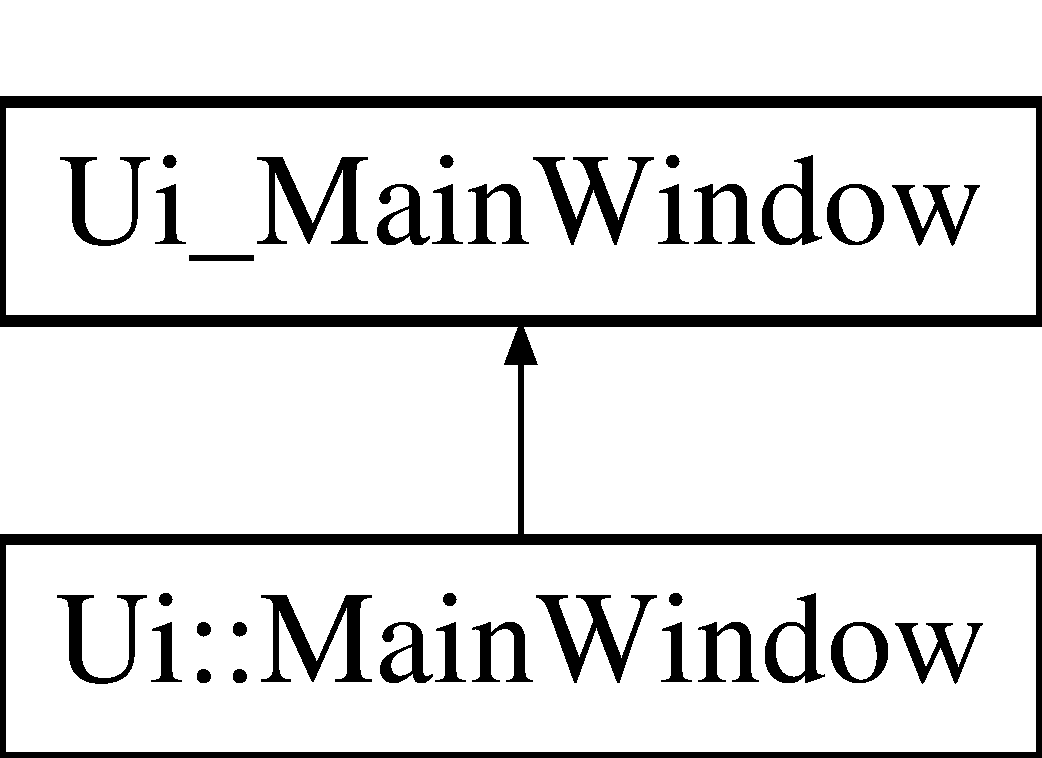
\includegraphics[height=2.000000cm]{class_ui_1_1_main_window}
\end{center}
\end{figure}
\subsection*{Additional Inherited Members}


The documentation for this class was generated from the following file\+:\begin{DoxyCompactItemize}
\item 
\hyperlink{ui__mainwindow_8h}{ui\+\_\+mainwindow.\+h}\end{DoxyCompactItemize}

\hypertarget{class_object_settings}{}\section{Object\+Settings Class Reference}
\label{class_object_settings}\index{Object\+Settings@{Object\+Settings}}


The \hyperlink{class_object_settings}{Object\+Settings} class.  




{\ttfamily \#include $<$objectsettings.\+h$>$}

Inheritance diagram for Object\+Settings\+:\begin{figure}[H]
\begin{center}
\leavevmode
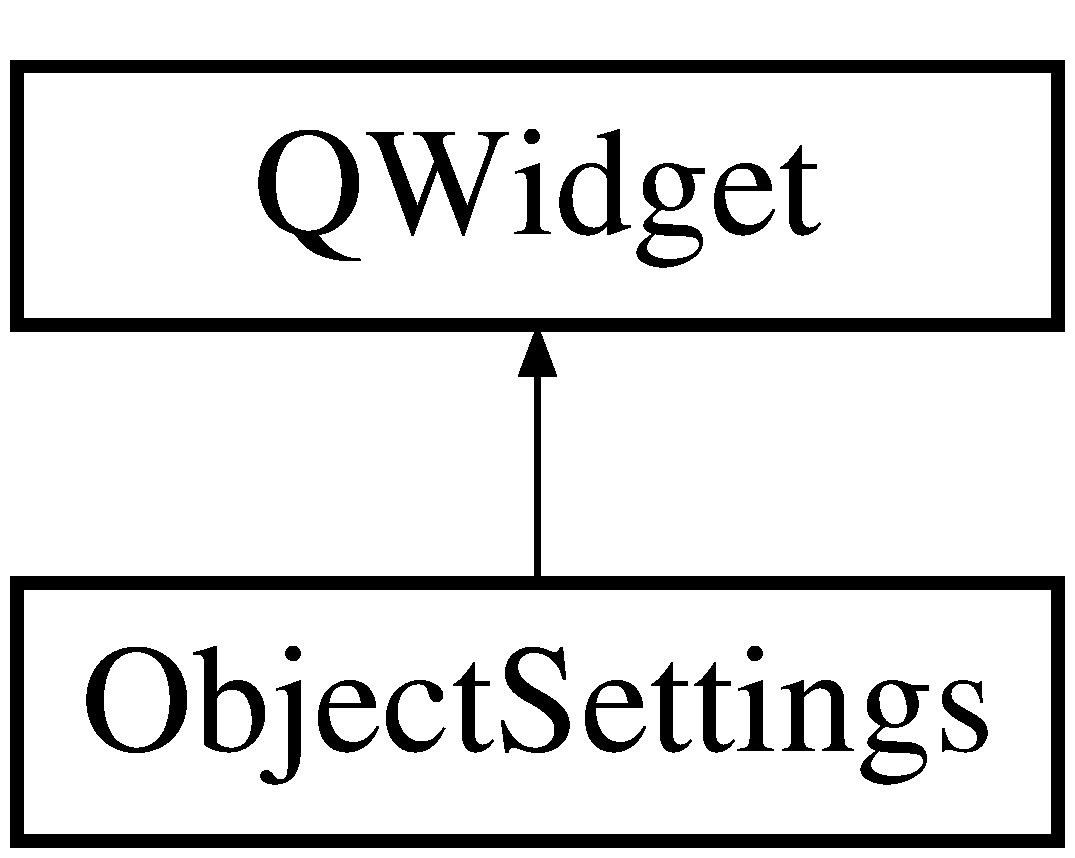
\includegraphics[height=2.000000cm]{class_object_settings}
\end{center}
\end{figure}
\subsection*{Public Slots}
\begin{DoxyCompactItemize}
\item 
void \hyperlink{class_object_settings_a47aec256bb36db5eda17686a38294932}{object\+Attributes} (\hyperlink{class_graphics_object}{Graphics\+Object} $\ast$my\+Object)
\end{DoxyCompactItemize}
\subsection*{Signals}
\begin{DoxyCompactItemize}
\item 
void \hyperlink{class_object_settings_a0b6604a8c84bd495e744fbe3012eca89}{my\+Object\+Name\+Changed} (Q\+String arg1)
\item 
void \hyperlink{class_object_settings_a748b6c75fd1d8a63314f1ebd585c51ce}{pb\+\_\+remove\+Object} ()
\item 
void \hyperlink{class_object_settings_a951847088536bc75bea1cf55418e895f}{dial\+\_\+rotation\+Changed} (int value)
\item 
void \hyperlink{class_object_settings_aaf878088ff438a5508f51cd9b639497e}{close\+Button\+Pressed} ()
\end{DoxyCompactItemize}
\subsection*{Public Member Functions}
\begin{DoxyCompactItemize}
\item 
\hyperlink{class_object_settings_aa7ea354843a408eeac937c76de954eeb}{Object\+Settings} (Q\+Widget $\ast$parent=0)
\item 
\hyperlink{class_object_settings_ad93bcbc973825c0052c246039fe6d4d0}{$\sim$\+Object\+Settings} ()
\end{DoxyCompactItemize}


\subsection{Detailed Description}
The \hyperlink{class_object_settings}{Object\+Settings} class. 

\subsection{Constructor \& Destructor Documentation}
\mbox{\Hypertarget{class_object_settings_aa7ea354843a408eeac937c76de954eeb}\label{class_object_settings_aa7ea354843a408eeac937c76de954eeb}} 
\index{Object\+Settings@{Object\+Settings}!Object\+Settings@{Object\+Settings}}
\index{Object\+Settings@{Object\+Settings}!Object\+Settings@{Object\+Settings}}
\subsubsection{\texorpdfstring{Object\+Settings()}{ObjectSettings()}}
{\footnotesize\ttfamily Object\+Settings\+::\+Object\+Settings (\begin{DoxyParamCaption}\item[{Q\+Widget $\ast$}]{parent = {\ttfamily 0} }\end{DoxyParamCaption})\hspace{0.3cm}{\ttfamily [explicit]}}

\mbox{\Hypertarget{class_object_settings_ad93bcbc973825c0052c246039fe6d4d0}\label{class_object_settings_ad93bcbc973825c0052c246039fe6d4d0}} 
\index{Object\+Settings@{Object\+Settings}!````~Object\+Settings@{$\sim$\+Object\+Settings}}
\index{````~Object\+Settings@{$\sim$\+Object\+Settings}!Object\+Settings@{Object\+Settings}}
\subsubsection{\texorpdfstring{$\sim$\+Object\+Settings()}{~ObjectSettings()}}
{\footnotesize\ttfamily Object\+Settings\+::$\sim$\+Object\+Settings (\begin{DoxyParamCaption}{ }\end{DoxyParamCaption})}



\subsection{Member Function Documentation}
\mbox{\Hypertarget{class_object_settings_aaf878088ff438a5508f51cd9b639497e}\label{class_object_settings_aaf878088ff438a5508f51cd9b639497e}} 
\index{Object\+Settings@{Object\+Settings}!close\+Button\+Pressed@{close\+Button\+Pressed}}
\index{close\+Button\+Pressed@{close\+Button\+Pressed}!Object\+Settings@{Object\+Settings}}
\subsubsection{\texorpdfstring{close\+Button\+Pressed}{closeButtonPressed}}
{\footnotesize\ttfamily void Object\+Settings\+::close\+Button\+Pressed (\begin{DoxyParamCaption}{ }\end{DoxyParamCaption})\hspace{0.3cm}{\ttfamily [signal]}}

\mbox{\Hypertarget{class_object_settings_a951847088536bc75bea1cf55418e895f}\label{class_object_settings_a951847088536bc75bea1cf55418e895f}} 
\index{Object\+Settings@{Object\+Settings}!dial\+\_\+rotation\+Changed@{dial\+\_\+rotation\+Changed}}
\index{dial\+\_\+rotation\+Changed@{dial\+\_\+rotation\+Changed}!Object\+Settings@{Object\+Settings}}
\subsubsection{\texorpdfstring{dial\+\_\+rotation\+Changed}{dial\_rotationChanged}}
{\footnotesize\ttfamily void Object\+Settings\+::dial\+\_\+rotation\+Changed (\begin{DoxyParamCaption}\item[{int}]{value }\end{DoxyParamCaption})\hspace{0.3cm}{\ttfamily [signal]}}

\mbox{\Hypertarget{class_object_settings_a0b6604a8c84bd495e744fbe3012eca89}\label{class_object_settings_a0b6604a8c84bd495e744fbe3012eca89}} 
\index{Object\+Settings@{Object\+Settings}!my\+Object\+Name\+Changed@{my\+Object\+Name\+Changed}}
\index{my\+Object\+Name\+Changed@{my\+Object\+Name\+Changed}!Object\+Settings@{Object\+Settings}}
\subsubsection{\texorpdfstring{my\+Object\+Name\+Changed}{myObjectNameChanged}}
{\footnotesize\ttfamily void Object\+Settings\+::my\+Object\+Name\+Changed (\begin{DoxyParamCaption}\item[{Q\+String}]{arg1 }\end{DoxyParamCaption})\hspace{0.3cm}{\ttfamily [signal]}}

\mbox{\Hypertarget{class_object_settings_a47aec256bb36db5eda17686a38294932}\label{class_object_settings_a47aec256bb36db5eda17686a38294932}} 
\index{Object\+Settings@{Object\+Settings}!object\+Attributes@{object\+Attributes}}
\index{object\+Attributes@{object\+Attributes}!Object\+Settings@{Object\+Settings}}
\subsubsection{\texorpdfstring{object\+Attributes}{objectAttributes}}
{\footnotesize\ttfamily void Object\+Settings\+::object\+Attributes (\begin{DoxyParamCaption}\item[{\hyperlink{class_graphics_object}{Graphics\+Object} $\ast$}]{my\+Object }\end{DoxyParamCaption})\hspace{0.3cm}{\ttfamily [slot]}}

\mbox{\Hypertarget{class_object_settings_a748b6c75fd1d8a63314f1ebd585c51ce}\label{class_object_settings_a748b6c75fd1d8a63314f1ebd585c51ce}} 
\index{Object\+Settings@{Object\+Settings}!pb\+\_\+remove\+Object@{pb\+\_\+remove\+Object}}
\index{pb\+\_\+remove\+Object@{pb\+\_\+remove\+Object}!Object\+Settings@{Object\+Settings}}
\subsubsection{\texorpdfstring{pb\+\_\+remove\+Object}{pb\_removeObject}}
{\footnotesize\ttfamily void Object\+Settings\+::pb\+\_\+remove\+Object (\begin{DoxyParamCaption}{ }\end{DoxyParamCaption})\hspace{0.3cm}{\ttfamily [signal]}}



The documentation for this class was generated from the following files\+:\begin{DoxyCompactItemize}
\item 
\hyperlink{objectsettings_8h}{objectsettings.\+h}\item 
\hyperlink{objectsettings_8cpp}{objectsettings.\+cpp}\end{DoxyCompactItemize}

\hypertarget{class_ui_1_1_object_settings}{}\section{Ui\+:\+:Object\+Settings Class Reference}
\label{class_ui_1_1_object_settings}\index{Ui\+::\+Object\+Settings@{Ui\+::\+Object\+Settings}}


{\ttfamily \#include $<$ui\+\_\+objectsettings.\+h$>$}

Inheritance diagram for Ui\+:\+:Object\+Settings\+:\begin{figure}[H]
\begin{center}
\leavevmode
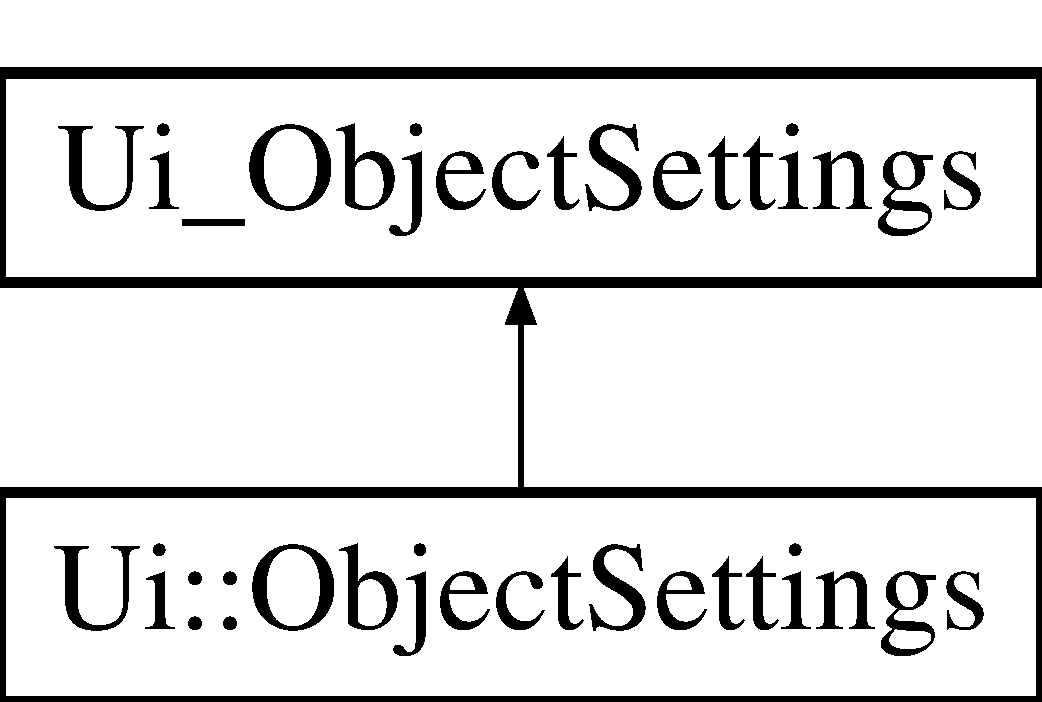
\includegraphics[height=2.000000cm]{class_ui_1_1_object_settings}
\end{center}
\end{figure}
\subsection*{Additional Inherited Members}


The documentation for this class was generated from the following file\+:\begin{DoxyCompactItemize}
\item 
\hyperlink{ui__objectsettings_8h}{ui\+\_\+objectsettings.\+h}\end{DoxyCompactItemize}

\hypertarget{class_rectangle}{}\section{Rectangle Class Reference}
\label{class_rectangle}\index{Rectangle@{Rectangle}}


The \hyperlink{class_rectangle}{Rectangle} class.  




{\ttfamily \#include $<$rectangle.\+h$>$}

Inheritance diagram for Rectangle\+:\begin{figure}[H]
\begin{center}
\leavevmode
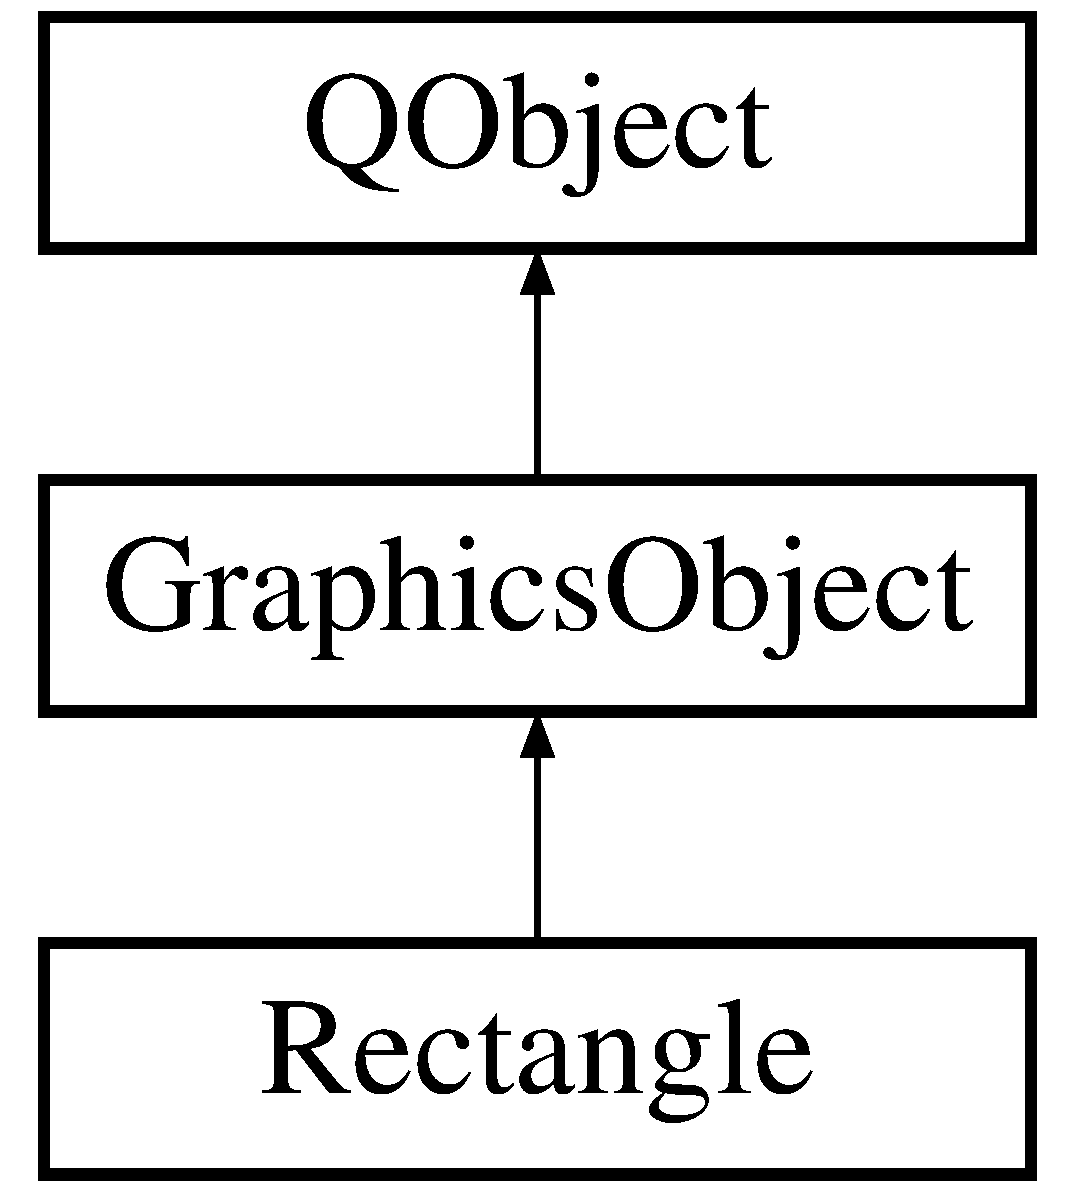
\includegraphics[height=3.000000cm]{class_rectangle}
\end{center}
\end{figure}
\subsection*{Public Member Functions}
\begin{DoxyCompactItemize}
\item 
\hyperlink{class_rectangle_af7b47bc1819c9c74311686ec33e6b921}{Rectangle} (Q\+Object $\ast$parent=0)
\begin{DoxyCompactList}\small\item\em Generates a new \hyperlink{class_rectangle}{Rectangle} Object. \end{DoxyCompactList}\item 
\hyperlink{class_rectangle_a5338f8ff5aa04be36032562617fe0603}{Rectangle} (qreal x, qreal y, qreal width, qreal heigth, Q\+Color color1, Q\+Color color2)
\item 
virtual Q\+Graphics\+Item $\ast$ \hyperlink{class_rectangle_a6d2cdec338bb43ad533b98e58eea9e03}{graphics\+Item} () const
\begin{DoxyCompactList}\small\item\em \hyperlink{class_graphics_object_abd625951730f006e748570bf00d158bf}{Graphics\+Object\+::graphics\+Item}. \end{DoxyCompactList}\item 
Q\+String \hyperlink{class_rectangle_a75b1e77ef828ff8de86cfcf6b03bfadb}{to\+String} ()
\end{DoxyCompactItemize}


\subsection{Detailed Description}
The \hyperlink{class_rectangle}{Rectangle} class. 

\subsection{Constructor \& Destructor Documentation}
\mbox{\Hypertarget{class_rectangle_af7b47bc1819c9c74311686ec33e6b921}\label{class_rectangle_af7b47bc1819c9c74311686ec33e6b921}} 
\index{Rectangle@{Rectangle}!Rectangle@{Rectangle}}
\index{Rectangle@{Rectangle}!Rectangle@{Rectangle}}
\subsubsection{\texorpdfstring{Rectangle()}{Rectangle()}\hspace{0.1cm}{\footnotesize\ttfamily [1/2]}}
{\footnotesize\ttfamily Rectangle\+::\+Rectangle (\begin{DoxyParamCaption}\item[{Q\+Object $\ast$}]{parent = {\ttfamily 0} }\end{DoxyParamCaption})\hspace{0.3cm}{\ttfamily [explicit]}}



Generates a new \hyperlink{class_rectangle}{Rectangle} Object. 


\begin{DoxyParams}{Parameters}
{\em parent} & \\
\hline
\end{DoxyParams}
\mbox{\Hypertarget{class_rectangle_a5338f8ff5aa04be36032562617fe0603}\label{class_rectangle_a5338f8ff5aa04be36032562617fe0603}} 
\index{Rectangle@{Rectangle}!Rectangle@{Rectangle}}
\index{Rectangle@{Rectangle}!Rectangle@{Rectangle}}
\subsubsection{\texorpdfstring{Rectangle()}{Rectangle()}\hspace{0.1cm}{\footnotesize\ttfamily [2/2]}}
{\footnotesize\ttfamily Rectangle\+::\+Rectangle (\begin{DoxyParamCaption}\item[{qreal}]{x,  }\item[{qreal}]{y,  }\item[{qreal}]{width,  }\item[{qreal}]{heigth,  }\item[{Q\+Color}]{color1,  }\item[{Q\+Color}]{color2 }\end{DoxyParamCaption})}



\subsection{Member Function Documentation}
\mbox{\Hypertarget{class_rectangle_a6d2cdec338bb43ad533b98e58eea9e03}\label{class_rectangle_a6d2cdec338bb43ad533b98e58eea9e03}} 
\index{Rectangle@{Rectangle}!graphics\+Item@{graphics\+Item}}
\index{graphics\+Item@{graphics\+Item}!Rectangle@{Rectangle}}
\subsubsection{\texorpdfstring{graphics\+Item()}{graphicsItem()}}
{\footnotesize\ttfamily Q\+Graphics\+Item $\ast$ Rectangle\+::graphics\+Item (\begin{DoxyParamCaption}{ }\end{DoxyParamCaption}) const\hspace{0.3cm}{\ttfamily [virtual]}}



\hyperlink{class_graphics_object_abd625951730f006e748570bf00d158bf}{Graphics\+Object\+::graphics\+Item}. 

\begin{DoxyReturn}{Returns}

\end{DoxyReturn}


Reimplemented from \hyperlink{class_graphics_object_abd625951730f006e748570bf00d158bf}{Graphics\+Object}.

\mbox{\Hypertarget{class_rectangle_a75b1e77ef828ff8de86cfcf6b03bfadb}\label{class_rectangle_a75b1e77ef828ff8de86cfcf6b03bfadb}} 
\index{Rectangle@{Rectangle}!to\+String@{to\+String}}
\index{to\+String@{to\+String}!Rectangle@{Rectangle}}
\subsubsection{\texorpdfstring{to\+String()}{toString()}}
{\footnotesize\ttfamily Q\+String Rectangle\+::to\+String (\begin{DoxyParamCaption}{ }\end{DoxyParamCaption})}



The documentation for this class was generated from the following files\+:\begin{DoxyCompactItemize}
\item 
\hyperlink{rectangle_8h}{rectangle.\+h}\item 
\hyperlink{rectangle_8cpp}{rectangle.\+cpp}\end{DoxyCompactItemize}

\hypertarget{class_room_groundplan}{}\section{Room\+Groundplan Class Reference}
\label{class_room_groundplan}\index{Room\+Groundplan@{Room\+Groundplan}}


The \hyperlink{class_room_groundplan}{Room\+Groundplan} class.  




{\ttfamily \#include $<$roomgroundplan.\+h$>$}

Inheritance diagram for Room\+Groundplan\+:\begin{figure}[H]
\begin{center}
\leavevmode
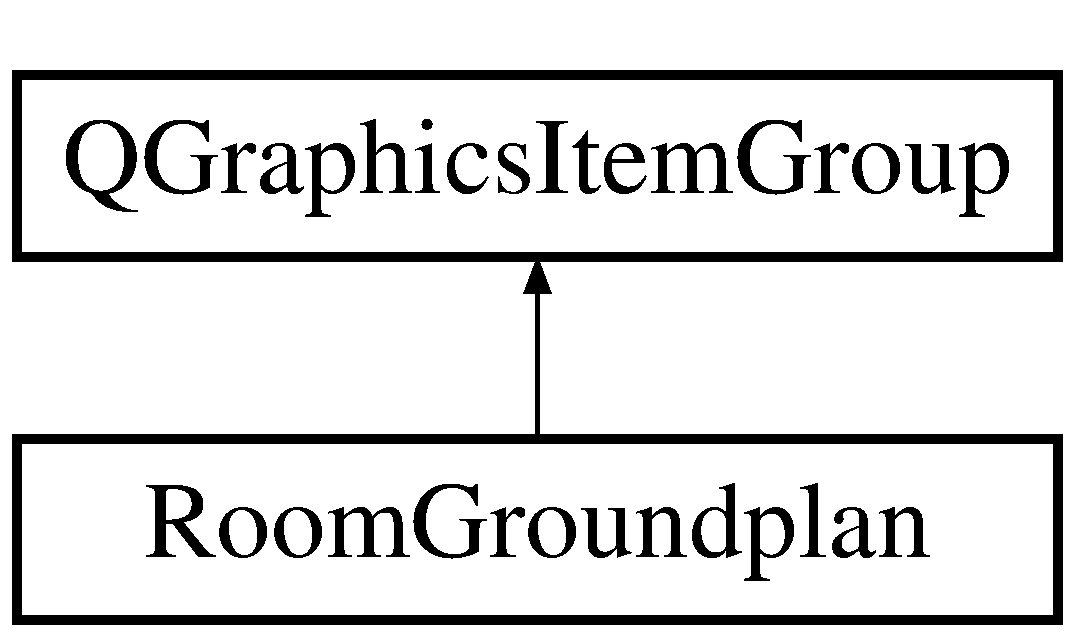
\includegraphics[height=2.000000cm]{class_room_groundplan}
\end{center}
\end{figure}
\subsection*{Public Member Functions}
\begin{DoxyCompactItemize}
\item 
\hyperlink{class_room_groundplan_a17876072e0ec924f8adbaa10ef0fb823}{Room\+Groundplan} (Q\+Graphics\+Item $\ast$parent=0)
\item 
void \hyperlink{class_room_groundplan_a5d9a4ec1560851a77f6797c41d713ac8}{add\+Line\+To\+Group} (Q\+PointF origin, Q\+PointF target)
\end{DoxyCompactItemize}


\subsection{Detailed Description}
The \hyperlink{class_room_groundplan}{Room\+Groundplan} class. 

\subsection{Constructor \& Destructor Documentation}
\mbox{\Hypertarget{class_room_groundplan_a17876072e0ec924f8adbaa10ef0fb823}\label{class_room_groundplan_a17876072e0ec924f8adbaa10ef0fb823}} 
\index{Room\+Groundplan@{Room\+Groundplan}!Room\+Groundplan@{Room\+Groundplan}}
\index{Room\+Groundplan@{Room\+Groundplan}!Room\+Groundplan@{Room\+Groundplan}}
\subsubsection{\texorpdfstring{Room\+Groundplan()}{RoomGroundplan()}}
{\footnotesize\ttfamily Room\+Groundplan\+::\+Room\+Groundplan (\begin{DoxyParamCaption}\item[{Q\+Graphics\+Item $\ast$}]{parent = {\ttfamily 0} }\end{DoxyParamCaption})}



\subsection{Member Function Documentation}
\mbox{\Hypertarget{class_room_groundplan_a5d9a4ec1560851a77f6797c41d713ac8}\label{class_room_groundplan_a5d9a4ec1560851a77f6797c41d713ac8}} 
\index{Room\+Groundplan@{Room\+Groundplan}!add\+Line\+To\+Group@{add\+Line\+To\+Group}}
\index{add\+Line\+To\+Group@{add\+Line\+To\+Group}!Room\+Groundplan@{Room\+Groundplan}}
\subsubsection{\texorpdfstring{add\+Line\+To\+Group()}{addLineToGroup()}}
{\footnotesize\ttfamily void Room\+Groundplan\+::add\+Line\+To\+Group (\begin{DoxyParamCaption}\item[{Q\+PointF}]{origin,  }\item[{Q\+PointF}]{target }\end{DoxyParamCaption})}



The documentation for this class was generated from the following files\+:\begin{DoxyCompactItemize}
\item 
\hyperlink{roomgroundplan_8h}{roomgroundplan.\+h}\item 
\hyperlink{roomgroundplan_8cpp}{roomgroundplan.\+cpp}\end{DoxyCompactItemize}

\hypertarget{class_ui_1_1_tutorial_line_tool}{}\section{Ui\+:\+:Tutorial\+Line\+Tool Class Reference}
\label{class_ui_1_1_tutorial_line_tool}\index{Ui\+::\+Tutorial\+Line\+Tool@{Ui\+::\+Tutorial\+Line\+Tool}}


{\ttfamily \#include $<$ui\+\_\+tutoriallinetool.\+h$>$}

Inheritance diagram for Ui\+:\+:Tutorial\+Line\+Tool\+:\begin{figure}[H]
\begin{center}
\leavevmode
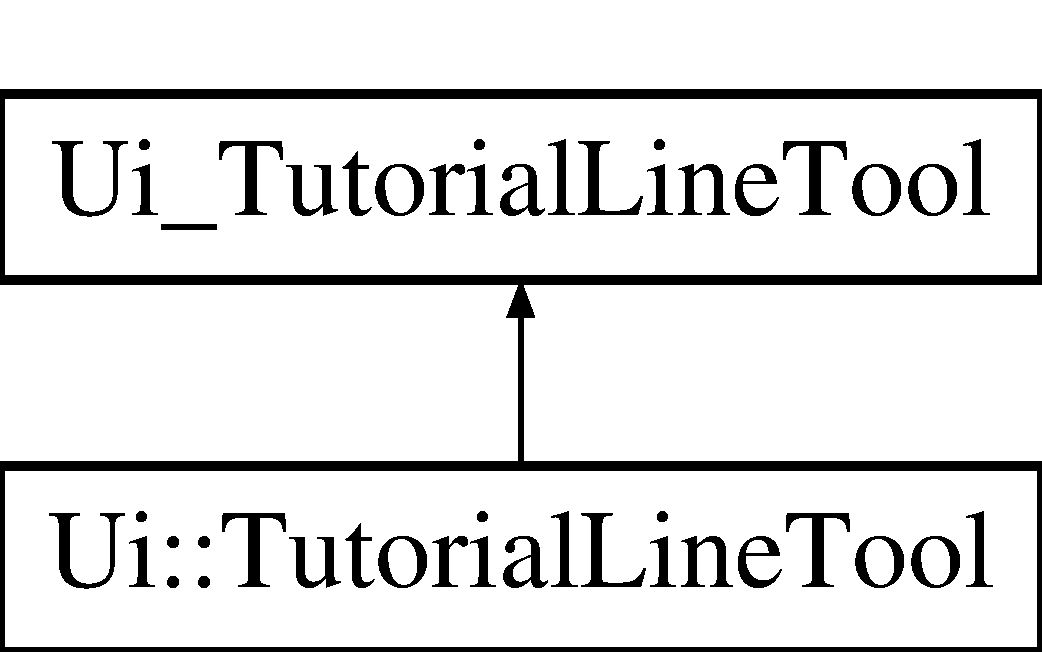
\includegraphics[height=2.000000cm]{class_ui_1_1_tutorial_line_tool}
\end{center}
\end{figure}
\subsection*{Additional Inherited Members}


The documentation for this class was generated from the following file\+:\begin{DoxyCompactItemize}
\item 
\hyperlink{ui__tutoriallinetool_8h}{ui\+\_\+tutoriallinetool.\+h}\end{DoxyCompactItemize}

\hypertarget{class_tutorial_line_tool}{}\section{Tutorial\+Line\+Tool Class Reference}
\label{class_tutorial_line_tool}\index{Tutorial\+Line\+Tool@{Tutorial\+Line\+Tool}}


The \hyperlink{class_tutorial_line_tool}{Tutorial\+Line\+Tool} class.  




{\ttfamily \#include $<$tutoriallinetool.\+h$>$}

Inheritance diagram for Tutorial\+Line\+Tool\+:\begin{figure}[H]
\begin{center}
\leavevmode
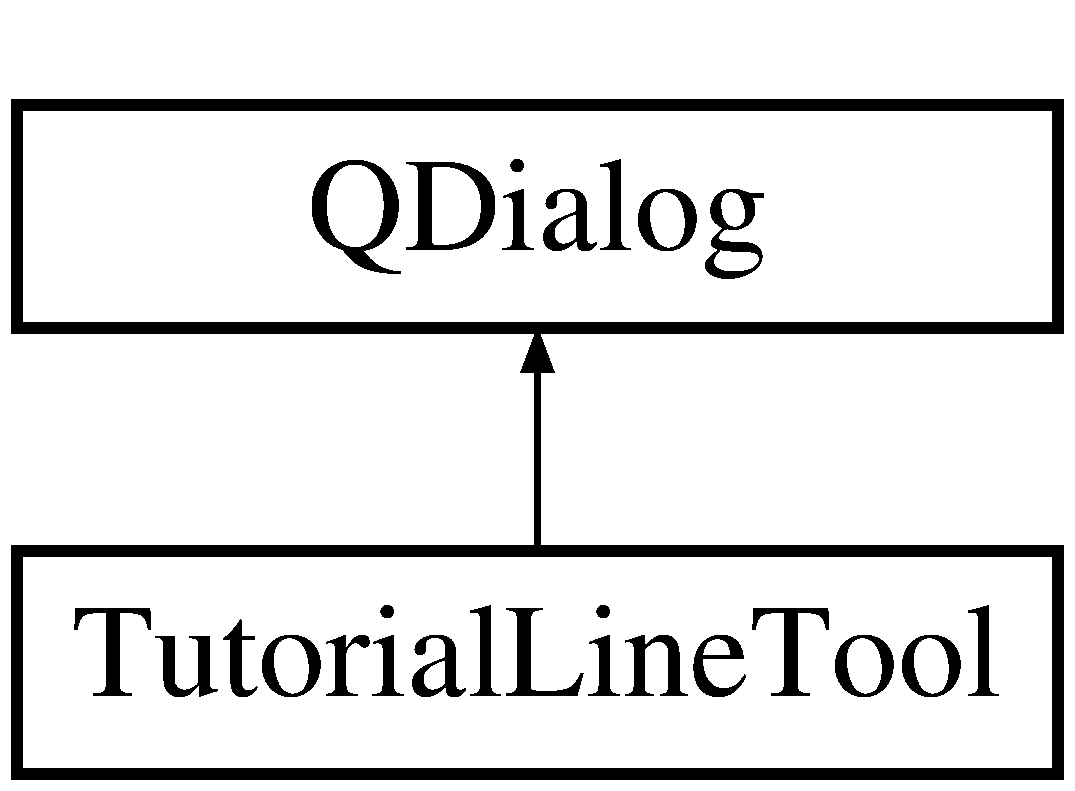
\includegraphics[height=2.000000cm]{class_tutorial_line_tool}
\end{center}
\end{figure}
\subsection*{Public Member Functions}
\begin{DoxyCompactItemize}
\item 
\hyperlink{class_tutorial_line_tool_af4e5c2a7e79544e7c6fc7e21d0007347}{Tutorial\+Line\+Tool} (Q\+Widget $\ast$parent=0)
\item 
\hyperlink{class_tutorial_line_tool_a03f51cf61b5bbf1798e86452195aeef2}{$\sim$\+Tutorial\+Line\+Tool} ()
\end{DoxyCompactItemize}


\subsection{Detailed Description}
The \hyperlink{class_tutorial_line_tool}{Tutorial\+Line\+Tool} class. 

\subsection{Constructor \& Destructor Documentation}
\mbox{\Hypertarget{class_tutorial_line_tool_af4e5c2a7e79544e7c6fc7e21d0007347}\label{class_tutorial_line_tool_af4e5c2a7e79544e7c6fc7e21d0007347}} 
\index{Tutorial\+Line\+Tool@{Tutorial\+Line\+Tool}!Tutorial\+Line\+Tool@{Tutorial\+Line\+Tool}}
\index{Tutorial\+Line\+Tool@{Tutorial\+Line\+Tool}!Tutorial\+Line\+Tool@{Tutorial\+Line\+Tool}}
\subsubsection{\texorpdfstring{Tutorial\+Line\+Tool()}{TutorialLineTool()}}
{\footnotesize\ttfamily Tutorial\+Line\+Tool\+::\+Tutorial\+Line\+Tool (\begin{DoxyParamCaption}\item[{Q\+Widget $\ast$}]{parent = {\ttfamily 0} }\end{DoxyParamCaption})\hspace{0.3cm}{\ttfamily [explicit]}}

\mbox{\Hypertarget{class_tutorial_line_tool_a03f51cf61b5bbf1798e86452195aeef2}\label{class_tutorial_line_tool_a03f51cf61b5bbf1798e86452195aeef2}} 
\index{Tutorial\+Line\+Tool@{Tutorial\+Line\+Tool}!````~Tutorial\+Line\+Tool@{$\sim$\+Tutorial\+Line\+Tool}}
\index{````~Tutorial\+Line\+Tool@{$\sim$\+Tutorial\+Line\+Tool}!Tutorial\+Line\+Tool@{Tutorial\+Line\+Tool}}
\subsubsection{\texorpdfstring{$\sim$\+Tutorial\+Line\+Tool()}{~TutorialLineTool()}}
{\footnotesize\ttfamily Tutorial\+Line\+Tool\+::$\sim$\+Tutorial\+Line\+Tool (\begin{DoxyParamCaption}{ }\end{DoxyParamCaption})}



The documentation for this class was generated from the following files\+:\begin{DoxyCompactItemize}
\item 
\hyperlink{tutoriallinetool_8h}{tutoriallinetool.\+h}\item 
\hyperlink{tutoriallinetool_8cpp}{tutoriallinetool.\+cpp}\end{DoxyCompactItemize}

\hypertarget{class_ui___color_tool_selector}{}\section{Ui\+\_\+\+Color\+Tool\+Selector Class Reference}
\label{class_ui___color_tool_selector}\index{Ui\+\_\+\+Color\+Tool\+Selector@{Ui\+\_\+\+Color\+Tool\+Selector}}


{\ttfamily \#include $<$ui\+\_\+colortoolselector.\+h$>$}

Inheritance diagram for Ui\+\_\+\+Color\+Tool\+Selector\+:\begin{figure}[H]
\begin{center}
\leavevmode
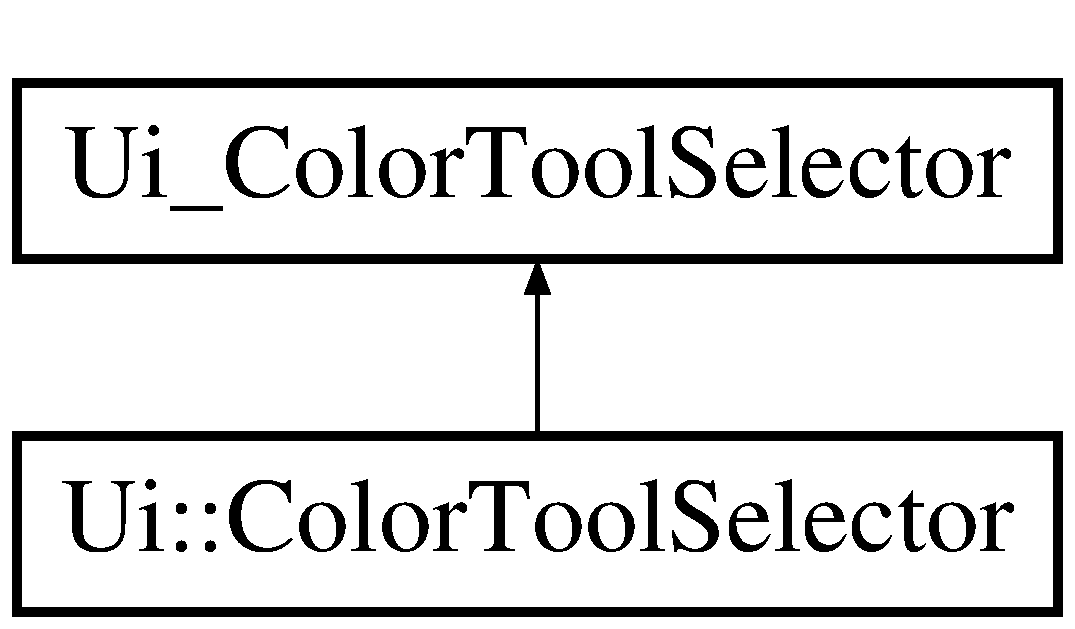
\includegraphics[height=2.000000cm]{class_ui___color_tool_selector}
\end{center}
\end{figure}
\subsection*{Public Member Functions}
\begin{DoxyCompactItemize}
\item 
void \hyperlink{class_ui___color_tool_selector_aa302dcf865058c72705f5cf9a3e07822}{setup\+Ui} (Q\+Widget $\ast$\hyperlink{class_color_tool_selector}{Color\+Tool\+Selector})
\item 
void \hyperlink{class_ui___color_tool_selector_ac18c0e3964ab075c31dbe5708e5bfa15}{retranslate\+Ui} (Q\+Widget $\ast$\hyperlink{class_color_tool_selector}{Color\+Tool\+Selector})
\end{DoxyCompactItemize}
\subsection*{Public Attributes}
\begin{DoxyCompactItemize}
\item 
Q\+Grid\+Layout $\ast$ \hyperlink{class_ui___color_tool_selector_a2c3286ab8dcdbca7dc2d6e07e2bbed49}{grid\+Layout}
\item 
Q\+Group\+Box $\ast$ \hyperlink{class_ui___color_tool_selector_a97d6fcbf9dbfe3ea8293ccd933bc2264}{group\+Box\+\_\+5}
\item 
Q\+V\+Box\+Layout $\ast$ \hyperlink{class_ui___color_tool_selector_a040c4849172e8f21adbd0c038f343c39}{vertical\+Layout}
\item 
Q\+Group\+Box $\ast$ \hyperlink{class_ui___color_tool_selector_a4564df0b9bd5e8f52e74d4eecedce1f0}{group\+Box\+\_\+2}
\item 
Q\+V\+Box\+Layout $\ast$ \hyperlink{class_ui___color_tool_selector_a3a1b911be3ed700de6315364a61999d9}{vertical\+Layout\+\_\+4}
\item 
\hyperlink{class_color_button}{Color\+Button} $\ast$ \hyperlink{class_ui___color_tool_selector_ad8fc8d84903bdcb9c7600d9690bbae58}{pb\+\_\+fill\+\_\+color}
\item 
Q\+Group\+Box $\ast$ \hyperlink{class_ui___color_tool_selector_a0eec723e0bf3b2d0df2c3c09b57b60f5}{group\+Box\+\_\+3}
\item 
Q\+V\+Box\+Layout $\ast$ \hyperlink{class_ui___color_tool_selector_a20890ac92d7000b22f64b8e9a5a3e703}{vertical\+Layout\+\_\+5}
\item 
\hyperlink{class_color_button}{Color\+Button} $\ast$ \hyperlink{class_ui___color_tool_selector_a2289ac77d2f44f84ff2d28b862bdc2d8}{pb\+\_\+border\+\_\+color}
\end{DoxyCompactItemize}


\subsection{Member Function Documentation}
\mbox{\Hypertarget{class_ui___color_tool_selector_ac18c0e3964ab075c31dbe5708e5bfa15}\label{class_ui___color_tool_selector_ac18c0e3964ab075c31dbe5708e5bfa15}} 
\index{Ui\+\_\+\+Color\+Tool\+Selector@{Ui\+\_\+\+Color\+Tool\+Selector}!retranslate\+Ui@{retranslate\+Ui}}
\index{retranslate\+Ui@{retranslate\+Ui}!Ui\+\_\+\+Color\+Tool\+Selector@{Ui\+\_\+\+Color\+Tool\+Selector}}
\subsubsection{\texorpdfstring{retranslate\+Ui()}{retranslateUi()}}
{\footnotesize\ttfamily void Ui\+\_\+\+Color\+Tool\+Selector\+::retranslate\+Ui (\begin{DoxyParamCaption}\item[{Q\+Widget $\ast$}]{Color\+Tool\+Selector }\end{DoxyParamCaption})\hspace{0.3cm}{\ttfamily [inline]}}

\mbox{\Hypertarget{class_ui___color_tool_selector_aa302dcf865058c72705f5cf9a3e07822}\label{class_ui___color_tool_selector_aa302dcf865058c72705f5cf9a3e07822}} 
\index{Ui\+\_\+\+Color\+Tool\+Selector@{Ui\+\_\+\+Color\+Tool\+Selector}!setup\+Ui@{setup\+Ui}}
\index{setup\+Ui@{setup\+Ui}!Ui\+\_\+\+Color\+Tool\+Selector@{Ui\+\_\+\+Color\+Tool\+Selector}}
\subsubsection{\texorpdfstring{setup\+Ui()}{setupUi()}}
{\footnotesize\ttfamily void Ui\+\_\+\+Color\+Tool\+Selector\+::setup\+Ui (\begin{DoxyParamCaption}\item[{Q\+Widget $\ast$}]{Color\+Tool\+Selector }\end{DoxyParamCaption})\hspace{0.3cm}{\ttfamily [inline]}}



\subsection{Member Data Documentation}
\mbox{\Hypertarget{class_ui___color_tool_selector_a2c3286ab8dcdbca7dc2d6e07e2bbed49}\label{class_ui___color_tool_selector_a2c3286ab8dcdbca7dc2d6e07e2bbed49}} 
\index{Ui\+\_\+\+Color\+Tool\+Selector@{Ui\+\_\+\+Color\+Tool\+Selector}!grid\+Layout@{grid\+Layout}}
\index{grid\+Layout@{grid\+Layout}!Ui\+\_\+\+Color\+Tool\+Selector@{Ui\+\_\+\+Color\+Tool\+Selector}}
\subsubsection{\texorpdfstring{grid\+Layout}{gridLayout}}
{\footnotesize\ttfamily Q\+Grid\+Layout$\ast$ Ui\+\_\+\+Color\+Tool\+Selector\+::grid\+Layout}

\mbox{\Hypertarget{class_ui___color_tool_selector_a4564df0b9bd5e8f52e74d4eecedce1f0}\label{class_ui___color_tool_selector_a4564df0b9bd5e8f52e74d4eecedce1f0}} 
\index{Ui\+\_\+\+Color\+Tool\+Selector@{Ui\+\_\+\+Color\+Tool\+Selector}!group\+Box\+\_\+2@{group\+Box\+\_\+2}}
\index{group\+Box\+\_\+2@{group\+Box\+\_\+2}!Ui\+\_\+\+Color\+Tool\+Selector@{Ui\+\_\+\+Color\+Tool\+Selector}}
\subsubsection{\texorpdfstring{group\+Box\+\_\+2}{groupBox\_2}}
{\footnotesize\ttfamily Q\+Group\+Box$\ast$ Ui\+\_\+\+Color\+Tool\+Selector\+::group\+Box\+\_\+2}

\mbox{\Hypertarget{class_ui___color_tool_selector_a0eec723e0bf3b2d0df2c3c09b57b60f5}\label{class_ui___color_tool_selector_a0eec723e0bf3b2d0df2c3c09b57b60f5}} 
\index{Ui\+\_\+\+Color\+Tool\+Selector@{Ui\+\_\+\+Color\+Tool\+Selector}!group\+Box\+\_\+3@{group\+Box\+\_\+3}}
\index{group\+Box\+\_\+3@{group\+Box\+\_\+3}!Ui\+\_\+\+Color\+Tool\+Selector@{Ui\+\_\+\+Color\+Tool\+Selector}}
\subsubsection{\texorpdfstring{group\+Box\+\_\+3}{groupBox\_3}}
{\footnotesize\ttfamily Q\+Group\+Box$\ast$ Ui\+\_\+\+Color\+Tool\+Selector\+::group\+Box\+\_\+3}

\mbox{\Hypertarget{class_ui___color_tool_selector_a97d6fcbf9dbfe3ea8293ccd933bc2264}\label{class_ui___color_tool_selector_a97d6fcbf9dbfe3ea8293ccd933bc2264}} 
\index{Ui\+\_\+\+Color\+Tool\+Selector@{Ui\+\_\+\+Color\+Tool\+Selector}!group\+Box\+\_\+5@{group\+Box\+\_\+5}}
\index{group\+Box\+\_\+5@{group\+Box\+\_\+5}!Ui\+\_\+\+Color\+Tool\+Selector@{Ui\+\_\+\+Color\+Tool\+Selector}}
\subsubsection{\texorpdfstring{group\+Box\+\_\+5}{groupBox\_5}}
{\footnotesize\ttfamily Q\+Group\+Box$\ast$ Ui\+\_\+\+Color\+Tool\+Selector\+::group\+Box\+\_\+5}

\mbox{\Hypertarget{class_ui___color_tool_selector_a2289ac77d2f44f84ff2d28b862bdc2d8}\label{class_ui___color_tool_selector_a2289ac77d2f44f84ff2d28b862bdc2d8}} 
\index{Ui\+\_\+\+Color\+Tool\+Selector@{Ui\+\_\+\+Color\+Tool\+Selector}!pb\+\_\+border\+\_\+color@{pb\+\_\+border\+\_\+color}}
\index{pb\+\_\+border\+\_\+color@{pb\+\_\+border\+\_\+color}!Ui\+\_\+\+Color\+Tool\+Selector@{Ui\+\_\+\+Color\+Tool\+Selector}}
\subsubsection{\texorpdfstring{pb\+\_\+border\+\_\+color}{pb\_border\_color}}
{\footnotesize\ttfamily \hyperlink{class_color_button}{Color\+Button}$\ast$ Ui\+\_\+\+Color\+Tool\+Selector\+::pb\+\_\+border\+\_\+color}

\mbox{\Hypertarget{class_ui___color_tool_selector_ad8fc8d84903bdcb9c7600d9690bbae58}\label{class_ui___color_tool_selector_ad8fc8d84903bdcb9c7600d9690bbae58}} 
\index{Ui\+\_\+\+Color\+Tool\+Selector@{Ui\+\_\+\+Color\+Tool\+Selector}!pb\+\_\+fill\+\_\+color@{pb\+\_\+fill\+\_\+color}}
\index{pb\+\_\+fill\+\_\+color@{pb\+\_\+fill\+\_\+color}!Ui\+\_\+\+Color\+Tool\+Selector@{Ui\+\_\+\+Color\+Tool\+Selector}}
\subsubsection{\texorpdfstring{pb\+\_\+fill\+\_\+color}{pb\_fill\_color}}
{\footnotesize\ttfamily \hyperlink{class_color_button}{Color\+Button}$\ast$ Ui\+\_\+\+Color\+Tool\+Selector\+::pb\+\_\+fill\+\_\+color}

\mbox{\Hypertarget{class_ui___color_tool_selector_a040c4849172e8f21adbd0c038f343c39}\label{class_ui___color_tool_selector_a040c4849172e8f21adbd0c038f343c39}} 
\index{Ui\+\_\+\+Color\+Tool\+Selector@{Ui\+\_\+\+Color\+Tool\+Selector}!vertical\+Layout@{vertical\+Layout}}
\index{vertical\+Layout@{vertical\+Layout}!Ui\+\_\+\+Color\+Tool\+Selector@{Ui\+\_\+\+Color\+Tool\+Selector}}
\subsubsection{\texorpdfstring{vertical\+Layout}{verticalLayout}}
{\footnotesize\ttfamily Q\+V\+Box\+Layout$\ast$ Ui\+\_\+\+Color\+Tool\+Selector\+::vertical\+Layout}

\mbox{\Hypertarget{class_ui___color_tool_selector_a3a1b911be3ed700de6315364a61999d9}\label{class_ui___color_tool_selector_a3a1b911be3ed700de6315364a61999d9}} 
\index{Ui\+\_\+\+Color\+Tool\+Selector@{Ui\+\_\+\+Color\+Tool\+Selector}!vertical\+Layout\+\_\+4@{vertical\+Layout\+\_\+4}}
\index{vertical\+Layout\+\_\+4@{vertical\+Layout\+\_\+4}!Ui\+\_\+\+Color\+Tool\+Selector@{Ui\+\_\+\+Color\+Tool\+Selector}}
\subsubsection{\texorpdfstring{vertical\+Layout\+\_\+4}{verticalLayout\_4}}
{\footnotesize\ttfamily Q\+V\+Box\+Layout$\ast$ Ui\+\_\+\+Color\+Tool\+Selector\+::vertical\+Layout\+\_\+4}

\mbox{\Hypertarget{class_ui___color_tool_selector_a20890ac92d7000b22f64b8e9a5a3e703}\label{class_ui___color_tool_selector_a20890ac92d7000b22f64b8e9a5a3e703}} 
\index{Ui\+\_\+\+Color\+Tool\+Selector@{Ui\+\_\+\+Color\+Tool\+Selector}!vertical\+Layout\+\_\+5@{vertical\+Layout\+\_\+5}}
\index{vertical\+Layout\+\_\+5@{vertical\+Layout\+\_\+5}!Ui\+\_\+\+Color\+Tool\+Selector@{Ui\+\_\+\+Color\+Tool\+Selector}}
\subsubsection{\texorpdfstring{vertical\+Layout\+\_\+5}{verticalLayout\_5}}
{\footnotesize\ttfamily Q\+V\+Box\+Layout$\ast$ Ui\+\_\+\+Color\+Tool\+Selector\+::vertical\+Layout\+\_\+5}



The documentation for this class was generated from the following file\+:\begin{DoxyCompactItemize}
\item 
\hyperlink{ui__colortoolselector_8h}{ui\+\_\+colortoolselector.\+h}\end{DoxyCompactItemize}

\hypertarget{class_ui___drawing_tool_selector}{}\section{Ui\+\_\+\+Drawing\+Tool\+Selector Class Reference}
\label{class_ui___drawing_tool_selector}\index{Ui\+\_\+\+Drawing\+Tool\+Selector@{Ui\+\_\+\+Drawing\+Tool\+Selector}}


{\ttfamily \#include $<$ui\+\_\+drawingtoolselector.\+h$>$}

Inheritance diagram for Ui\+\_\+\+Drawing\+Tool\+Selector\+:\begin{figure}[H]
\begin{center}
\leavevmode
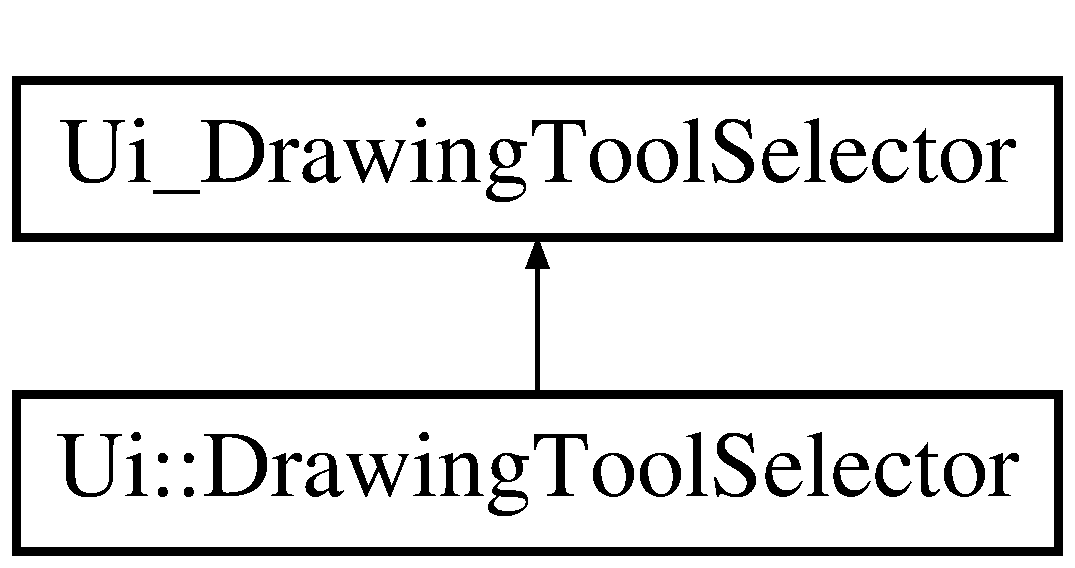
\includegraphics[height=2.000000cm]{class_ui___drawing_tool_selector}
\end{center}
\end{figure}
\subsection*{Public Member Functions}
\begin{DoxyCompactItemize}
\item 
void \hyperlink{class_ui___drawing_tool_selector_a370b1b8993d9c70f9da3d90e53a78686}{setup\+Ui} (Q\+Widget $\ast$\hyperlink{class_drawing_tool_selector}{Drawing\+Tool\+Selector})
\item 
void \hyperlink{class_ui___drawing_tool_selector_a3e822961e2773564eda0c30b90a25425}{retranslate\+Ui} (Q\+Widget $\ast$\hyperlink{class_drawing_tool_selector}{Drawing\+Tool\+Selector})
\end{DoxyCompactItemize}
\subsection*{Public Attributes}
\begin{DoxyCompactItemize}
\item 
Q\+Grid\+Layout $\ast$ \hyperlink{class_ui___drawing_tool_selector_a360ae3a69c31e336af215a424ce2ff9d}{grid\+Layout}
\item 
Q\+Group\+Box $\ast$ \hyperlink{class_ui___drawing_tool_selector_a1be65d4d8fd0c07e7fec52dd16000aaf}{group\+Box}
\item 
Q\+Grid\+Layout $\ast$ \hyperlink{class_ui___drawing_tool_selector_afbefb9a6b3cf7da7737ed2ded7d78a2d}{grid\+Layout\+\_\+4}
\item 
Q\+Label $\ast$ \hyperlink{class_ui___drawing_tool_selector_a02c26b2b0fccb633514b10fc1bd942a7}{label\+\_\+2}
\item 
Q\+Label $\ast$ \hyperlink{class_ui___drawing_tool_selector_a0b0d2d5d874fbe666cbcb6e28ca0c415}{label\+\_\+3}
\item 
Q\+Tool\+Button $\ast$ \hyperlink{class_ui___drawing_tool_selector_a2eafc39b04e16c7670823c5cd3ed702d}{pb\+\_\+circle}
\item 
Q\+Tool\+Button $\ast$ \hyperlink{class_ui___drawing_tool_selector_ab11a181c098447bd1f9aa184e976e0ad}{pb\+\_\+select}
\item 
Q\+Tool\+Button $\ast$ \hyperlink{class_ui___drawing_tool_selector_a17a31b8cff1a2d95abda193b33d36c0e}{pb\+\_\+rect}
\item 
Q\+Label $\ast$ \hyperlink{class_ui___drawing_tool_selector_aae76e8a3a9ecf2af48e1cd43227a8dad}{label}
\item 
Q\+Tool\+Button $\ast$ \hyperlink{class_ui___drawing_tool_selector_afbc78884825da33bd2d95206bfead3e7}{pb\+\_\+line}
\item 
Q\+Label $\ast$ \hyperlink{class_ui___drawing_tool_selector_ab0dafaa90171cf18ca7eff07e4e27512}{label\+\_\+4}
\end{DoxyCompactItemize}


\subsection{Member Function Documentation}
\mbox{\Hypertarget{class_ui___drawing_tool_selector_a3e822961e2773564eda0c30b90a25425}\label{class_ui___drawing_tool_selector_a3e822961e2773564eda0c30b90a25425}} 
\index{Ui\+\_\+\+Drawing\+Tool\+Selector@{Ui\+\_\+\+Drawing\+Tool\+Selector}!retranslate\+Ui@{retranslate\+Ui}}
\index{retranslate\+Ui@{retranslate\+Ui}!Ui\+\_\+\+Drawing\+Tool\+Selector@{Ui\+\_\+\+Drawing\+Tool\+Selector}}
\subsubsection{\texorpdfstring{retranslate\+Ui()}{retranslateUi()}}
{\footnotesize\ttfamily void Ui\+\_\+\+Drawing\+Tool\+Selector\+::retranslate\+Ui (\begin{DoxyParamCaption}\item[{Q\+Widget $\ast$}]{Drawing\+Tool\+Selector }\end{DoxyParamCaption})\hspace{0.3cm}{\ttfamily [inline]}}

\mbox{\Hypertarget{class_ui___drawing_tool_selector_a370b1b8993d9c70f9da3d90e53a78686}\label{class_ui___drawing_tool_selector_a370b1b8993d9c70f9da3d90e53a78686}} 
\index{Ui\+\_\+\+Drawing\+Tool\+Selector@{Ui\+\_\+\+Drawing\+Tool\+Selector}!setup\+Ui@{setup\+Ui}}
\index{setup\+Ui@{setup\+Ui}!Ui\+\_\+\+Drawing\+Tool\+Selector@{Ui\+\_\+\+Drawing\+Tool\+Selector}}
\subsubsection{\texorpdfstring{setup\+Ui()}{setupUi()}}
{\footnotesize\ttfamily void Ui\+\_\+\+Drawing\+Tool\+Selector\+::setup\+Ui (\begin{DoxyParamCaption}\item[{Q\+Widget $\ast$}]{Drawing\+Tool\+Selector }\end{DoxyParamCaption})\hspace{0.3cm}{\ttfamily [inline]}}



\subsection{Member Data Documentation}
\mbox{\Hypertarget{class_ui___drawing_tool_selector_a360ae3a69c31e336af215a424ce2ff9d}\label{class_ui___drawing_tool_selector_a360ae3a69c31e336af215a424ce2ff9d}} 
\index{Ui\+\_\+\+Drawing\+Tool\+Selector@{Ui\+\_\+\+Drawing\+Tool\+Selector}!grid\+Layout@{grid\+Layout}}
\index{grid\+Layout@{grid\+Layout}!Ui\+\_\+\+Drawing\+Tool\+Selector@{Ui\+\_\+\+Drawing\+Tool\+Selector}}
\subsubsection{\texorpdfstring{grid\+Layout}{gridLayout}}
{\footnotesize\ttfamily Q\+Grid\+Layout$\ast$ Ui\+\_\+\+Drawing\+Tool\+Selector\+::grid\+Layout}

\mbox{\Hypertarget{class_ui___drawing_tool_selector_afbefb9a6b3cf7da7737ed2ded7d78a2d}\label{class_ui___drawing_tool_selector_afbefb9a6b3cf7da7737ed2ded7d78a2d}} 
\index{Ui\+\_\+\+Drawing\+Tool\+Selector@{Ui\+\_\+\+Drawing\+Tool\+Selector}!grid\+Layout\+\_\+4@{grid\+Layout\+\_\+4}}
\index{grid\+Layout\+\_\+4@{grid\+Layout\+\_\+4}!Ui\+\_\+\+Drawing\+Tool\+Selector@{Ui\+\_\+\+Drawing\+Tool\+Selector}}
\subsubsection{\texorpdfstring{grid\+Layout\+\_\+4}{gridLayout\_4}}
{\footnotesize\ttfamily Q\+Grid\+Layout$\ast$ Ui\+\_\+\+Drawing\+Tool\+Selector\+::grid\+Layout\+\_\+4}

\mbox{\Hypertarget{class_ui___drawing_tool_selector_a1be65d4d8fd0c07e7fec52dd16000aaf}\label{class_ui___drawing_tool_selector_a1be65d4d8fd0c07e7fec52dd16000aaf}} 
\index{Ui\+\_\+\+Drawing\+Tool\+Selector@{Ui\+\_\+\+Drawing\+Tool\+Selector}!group\+Box@{group\+Box}}
\index{group\+Box@{group\+Box}!Ui\+\_\+\+Drawing\+Tool\+Selector@{Ui\+\_\+\+Drawing\+Tool\+Selector}}
\subsubsection{\texorpdfstring{group\+Box}{groupBox}}
{\footnotesize\ttfamily Q\+Group\+Box$\ast$ Ui\+\_\+\+Drawing\+Tool\+Selector\+::group\+Box}

\mbox{\Hypertarget{class_ui___drawing_tool_selector_aae76e8a3a9ecf2af48e1cd43227a8dad}\label{class_ui___drawing_tool_selector_aae76e8a3a9ecf2af48e1cd43227a8dad}} 
\index{Ui\+\_\+\+Drawing\+Tool\+Selector@{Ui\+\_\+\+Drawing\+Tool\+Selector}!label@{label}}
\index{label@{label}!Ui\+\_\+\+Drawing\+Tool\+Selector@{Ui\+\_\+\+Drawing\+Tool\+Selector}}
\subsubsection{\texorpdfstring{label}{label}}
{\footnotesize\ttfamily Q\+Label$\ast$ Ui\+\_\+\+Drawing\+Tool\+Selector\+::label}

\mbox{\Hypertarget{class_ui___drawing_tool_selector_a02c26b2b0fccb633514b10fc1bd942a7}\label{class_ui___drawing_tool_selector_a02c26b2b0fccb633514b10fc1bd942a7}} 
\index{Ui\+\_\+\+Drawing\+Tool\+Selector@{Ui\+\_\+\+Drawing\+Tool\+Selector}!label\+\_\+2@{label\+\_\+2}}
\index{label\+\_\+2@{label\+\_\+2}!Ui\+\_\+\+Drawing\+Tool\+Selector@{Ui\+\_\+\+Drawing\+Tool\+Selector}}
\subsubsection{\texorpdfstring{label\+\_\+2}{label\_2}}
{\footnotesize\ttfamily Q\+Label$\ast$ Ui\+\_\+\+Drawing\+Tool\+Selector\+::label\+\_\+2}

\mbox{\Hypertarget{class_ui___drawing_tool_selector_a0b0d2d5d874fbe666cbcb6e28ca0c415}\label{class_ui___drawing_tool_selector_a0b0d2d5d874fbe666cbcb6e28ca0c415}} 
\index{Ui\+\_\+\+Drawing\+Tool\+Selector@{Ui\+\_\+\+Drawing\+Tool\+Selector}!label\+\_\+3@{label\+\_\+3}}
\index{label\+\_\+3@{label\+\_\+3}!Ui\+\_\+\+Drawing\+Tool\+Selector@{Ui\+\_\+\+Drawing\+Tool\+Selector}}
\subsubsection{\texorpdfstring{label\+\_\+3}{label\_3}}
{\footnotesize\ttfamily Q\+Label$\ast$ Ui\+\_\+\+Drawing\+Tool\+Selector\+::label\+\_\+3}

\mbox{\Hypertarget{class_ui___drawing_tool_selector_ab0dafaa90171cf18ca7eff07e4e27512}\label{class_ui___drawing_tool_selector_ab0dafaa90171cf18ca7eff07e4e27512}} 
\index{Ui\+\_\+\+Drawing\+Tool\+Selector@{Ui\+\_\+\+Drawing\+Tool\+Selector}!label\+\_\+4@{label\+\_\+4}}
\index{label\+\_\+4@{label\+\_\+4}!Ui\+\_\+\+Drawing\+Tool\+Selector@{Ui\+\_\+\+Drawing\+Tool\+Selector}}
\subsubsection{\texorpdfstring{label\+\_\+4}{label\_4}}
{\footnotesize\ttfamily Q\+Label$\ast$ Ui\+\_\+\+Drawing\+Tool\+Selector\+::label\+\_\+4}

\mbox{\Hypertarget{class_ui___drawing_tool_selector_a2eafc39b04e16c7670823c5cd3ed702d}\label{class_ui___drawing_tool_selector_a2eafc39b04e16c7670823c5cd3ed702d}} 
\index{Ui\+\_\+\+Drawing\+Tool\+Selector@{Ui\+\_\+\+Drawing\+Tool\+Selector}!pb\+\_\+circle@{pb\+\_\+circle}}
\index{pb\+\_\+circle@{pb\+\_\+circle}!Ui\+\_\+\+Drawing\+Tool\+Selector@{Ui\+\_\+\+Drawing\+Tool\+Selector}}
\subsubsection{\texorpdfstring{pb\+\_\+circle}{pb\_circle}}
{\footnotesize\ttfamily Q\+Tool\+Button$\ast$ Ui\+\_\+\+Drawing\+Tool\+Selector\+::pb\+\_\+circle}

\mbox{\Hypertarget{class_ui___drawing_tool_selector_afbc78884825da33bd2d95206bfead3e7}\label{class_ui___drawing_tool_selector_afbc78884825da33bd2d95206bfead3e7}} 
\index{Ui\+\_\+\+Drawing\+Tool\+Selector@{Ui\+\_\+\+Drawing\+Tool\+Selector}!pb\+\_\+line@{pb\+\_\+line}}
\index{pb\+\_\+line@{pb\+\_\+line}!Ui\+\_\+\+Drawing\+Tool\+Selector@{Ui\+\_\+\+Drawing\+Tool\+Selector}}
\subsubsection{\texorpdfstring{pb\+\_\+line}{pb\_line}}
{\footnotesize\ttfamily Q\+Tool\+Button$\ast$ Ui\+\_\+\+Drawing\+Tool\+Selector\+::pb\+\_\+line}

\mbox{\Hypertarget{class_ui___drawing_tool_selector_a17a31b8cff1a2d95abda193b33d36c0e}\label{class_ui___drawing_tool_selector_a17a31b8cff1a2d95abda193b33d36c0e}} 
\index{Ui\+\_\+\+Drawing\+Tool\+Selector@{Ui\+\_\+\+Drawing\+Tool\+Selector}!pb\+\_\+rect@{pb\+\_\+rect}}
\index{pb\+\_\+rect@{pb\+\_\+rect}!Ui\+\_\+\+Drawing\+Tool\+Selector@{Ui\+\_\+\+Drawing\+Tool\+Selector}}
\subsubsection{\texorpdfstring{pb\+\_\+rect}{pb\_rect}}
{\footnotesize\ttfamily Q\+Tool\+Button$\ast$ Ui\+\_\+\+Drawing\+Tool\+Selector\+::pb\+\_\+rect}

\mbox{\Hypertarget{class_ui___drawing_tool_selector_ab11a181c098447bd1f9aa184e976e0ad}\label{class_ui___drawing_tool_selector_ab11a181c098447bd1f9aa184e976e0ad}} 
\index{Ui\+\_\+\+Drawing\+Tool\+Selector@{Ui\+\_\+\+Drawing\+Tool\+Selector}!pb\+\_\+select@{pb\+\_\+select}}
\index{pb\+\_\+select@{pb\+\_\+select}!Ui\+\_\+\+Drawing\+Tool\+Selector@{Ui\+\_\+\+Drawing\+Tool\+Selector}}
\subsubsection{\texorpdfstring{pb\+\_\+select}{pb\_select}}
{\footnotesize\ttfamily Q\+Tool\+Button$\ast$ Ui\+\_\+\+Drawing\+Tool\+Selector\+::pb\+\_\+select}



The documentation for this class was generated from the following file\+:\begin{DoxyCompactItemize}
\item 
\hyperlink{ui__drawingtoolselector_8h}{ui\+\_\+drawingtoolselector.\+h}\end{DoxyCompactItemize}

\hypertarget{class_ui___main_window}{}\section{Ui\+\_\+\+Main\+Window Class Reference}
\label{class_ui___main_window}\index{Ui\+\_\+\+Main\+Window@{Ui\+\_\+\+Main\+Window}}


{\ttfamily \#include $<$ui\+\_\+mainwindow.\+h$>$}

Inheritance diagram for Ui\+\_\+\+Main\+Window\+:\begin{figure}[H]
\begin{center}
\leavevmode
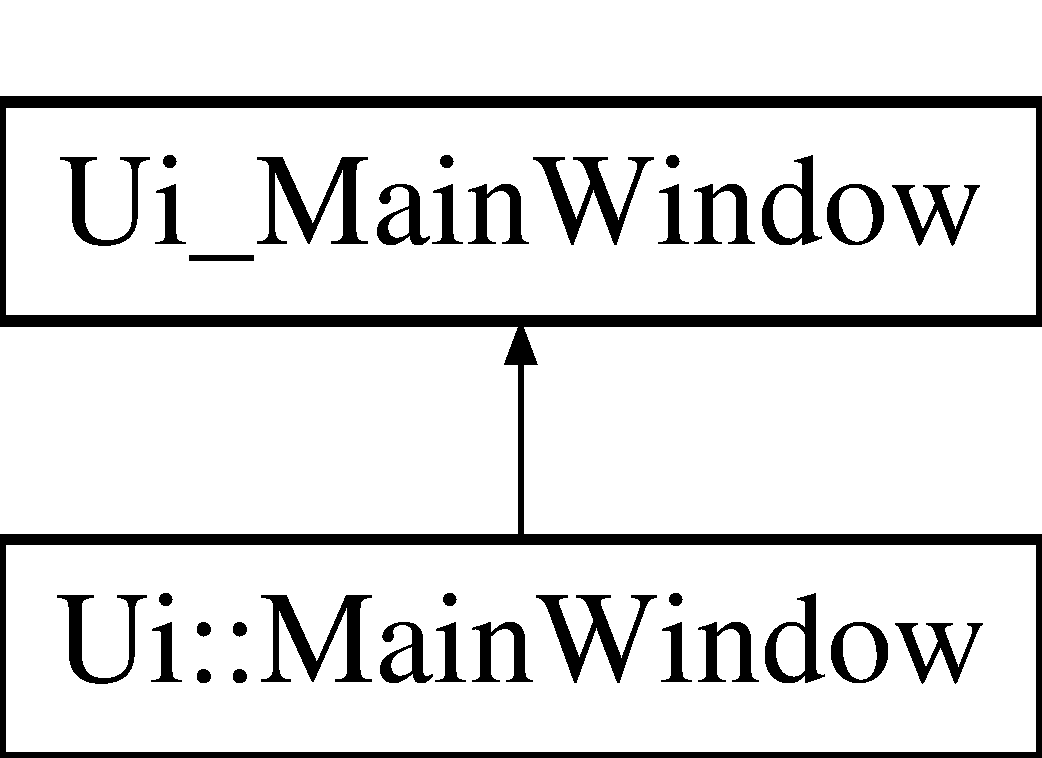
\includegraphics[height=2.000000cm]{class_ui___main_window}
\end{center}
\end{figure}
\subsection*{Public Member Functions}
\begin{DoxyCompactItemize}
\item 
void \hyperlink{class_ui___main_window_acf4a0872c4c77d8f43a2ec66ed849b58}{setup\+Ui} (Q\+Main\+Window $\ast$\hyperlink{class_main_window}{Main\+Window})
\item 
void \hyperlink{class_ui___main_window_a097dd160c3534a204904cb374412c618}{retranslate\+Ui} (Q\+Main\+Window $\ast$\hyperlink{class_main_window}{Main\+Window})
\end{DoxyCompactItemize}
\subsection*{Public Attributes}
\begin{DoxyCompactItemize}
\item 
Q\+Action $\ast$ \hyperlink{class_ui___main_window_a5772f39001f62b7f601aafe72caa10c0}{action\+Open}
\item 
Q\+Action $\ast$ \hyperlink{class_ui___main_window_a6e14788227f1a0dbc8cf983514685f3b}{action\+Save}
\item 
Q\+Action $\ast$ \hyperlink{class_ui___main_window_a2a918e9479b5de5c6171ee349d1a61f1}{action\+Select\+\_\+\+Tool}
\item 
Q\+Action $\ast$ \hyperlink{class_ui___main_window_adc1809dea2b94018b3fd6fc3efe40775}{action\+Circle\+\_\+\+Tool}
\item 
Q\+Action $\ast$ \hyperlink{class_ui___main_window_ac5febda9ff6ce44e31f0c3c1d889d388}{action\+Rectangle\+\_\+\+Tool}
\item 
Q\+Action $\ast$ \hyperlink{class_ui___main_window_ae8370529640da51b50cd1fb5be677c02}{action\+Exit}
\item 
Q\+Action $\ast$ \hyperlink{class_ui___main_window_a794b1c2e016ee1387008d1c22bec9b43}{action\+Line\+\_\+\+Tool}
\item 
Q\+Widget $\ast$ \hyperlink{class_ui___main_window_a30075506c2116c3ed4ff25e07ae75f81}{central\+Widget}
\item 
Q\+Grid\+Layout $\ast$ \hyperlink{class_ui___main_window_a525ed3c5fe0784ac502ee222fba4e205}{grid\+Layout}
\item 
Q\+Grid\+Layout $\ast$ \hyperlink{class_ui___main_window_af42ea7d4c2e893181caad21e28166932}{grid\+Layout\+\_\+3}
\item 
\hyperlink{class_drawing_tool_selector}{Drawing\+Tool\+Selector} $\ast$ \hyperlink{class_ui___main_window_ac1508256639e4341c10fb2b6ab66a646}{drawing\+Tool\+Selector}
\item 
\hyperlink{class_color_tool_selector}{Color\+Tool\+Selector} $\ast$ \hyperlink{class_ui___main_window_a7ae116c4161d4316369030c6c58d50f8}{color\+Tool\+Selector}
\item 
Q\+Grid\+Layout $\ast$ \hyperlink{class_ui___main_window_a6b2a0c5f7e8ff2a87134908dd770d2d2}{grid\+Layout\+\_\+2}
\item 
Q\+Grid\+Layout $\ast$ \hyperlink{class_ui___main_window_a8ee86315639f324b17708efc7dbe8b19}{grid\+Layout\+\_\+4}
\item 
Q\+Group\+Box $\ast$ \hyperlink{class_ui___main_window_afa8361dafeea9335501efa7f218549a8}{settings\+Box}
\item 
Q\+H\+Box\+Layout $\ast$ \hyperlink{class_ui___main_window_a80867018070156432923d0266cc9fe25}{horizontal\+Layout\+\_\+2}
\item 
Q\+Grid\+Layout $\ast$ \hyperlink{class_ui___main_window_ad113cf7b76aaf178473555bdf64ff035}{grid\+Layout\+\_\+6}
\item 
Q\+Double\+Spin\+Box $\ast$ \hyperlink{class_ui___main_window_a88ab1ae40c18d192579113661acff7e5}{sb\+\_\+x\+\_\+pos}
\item 
Q\+Label $\ast$ \hyperlink{class_ui___main_window_a4595b05b68b1fe0654f49880365f8bbf}{lb\+\_\+x\+\_\+pos}
\item 
Q\+Double\+Spin\+Box $\ast$ \hyperlink{class_ui___main_window_aace1213365524c7c202cb8ed1275d6c9}{sb\+\_\+y\+\_\+pos}
\item 
Q\+Label $\ast$ \hyperlink{class_ui___main_window_a87cfd1f185a4fdeea6cd518fab6d2f10}{lb\+\_\+y\+\_\+pos}
\item 
Q\+Spin\+Box $\ast$ \hyperlink{class_ui___main_window_a24b22ee2a2999c916f1856cdc9b30c1a}{sb\+\_\+width}
\item 
Q\+Label $\ast$ \hyperlink{class_ui___main_window_a61050b9dffa9937b28704c0add9edc92}{lb\+\_\+height}
\item 
Q\+Spin\+Box $\ast$ \hyperlink{class_ui___main_window_a4667610a26642e4588ba8ec79f8854c4}{sb\+\_\+heigth}
\item 
Q\+Label $\ast$ \hyperlink{class_ui___main_window_af1848a715d514f01db491648697a1678}{lb\+\_\+width}
\item 
Q\+Push\+Button $\ast$ \hyperlink{class_ui___main_window_a7943d7d8b767c4c7ceebe8123b31ae7f}{pb\+\_\+\+Add\+Object}
\item 
Q\+Push\+Button $\ast$ \hyperlink{class_ui___main_window_a59a7d8124bce933d63f53f2153d447b4}{push\+Button\+\_\+2}
\item 
Q\+Grid\+Layout $\ast$ \hyperlink{class_ui___main_window_a8731b71c513ff94baf59614807823c5d}{grid\+Layout\+\_\+5}
\item 
\hyperlink{class_object_settings}{Object\+Settings} $\ast$ \hyperlink{class_ui___main_window_ae99e485cd9af336f4b3b73911e44fe2d}{object\+Settings\+Widget}
\item 
Q\+Graphics\+View $\ast$ \hyperlink{class_ui___main_window_a713d8e541d9de8389ad4292131dc931a}{graphics\+View}
\item 
Q\+Menu\+Bar $\ast$ \hyperlink{class_ui___main_window_a2be1c24ec9adfca18e1dcc951931457f}{menu\+Bar}
\item 
Q\+Menu $\ast$ \hyperlink{class_ui___main_window_a7ba84cb4cdd6a12dc83bf4e100bd8d80}{menu\+File}
\item 
Q\+Menu $\ast$ \hyperlink{class_ui___main_window_a2d61dddc70dd5d135cded37470cc8f02}{menu\+Tool}
\item 
Q\+Tool\+Bar $\ast$ \hyperlink{class_ui___main_window_a5172877001c8c7b4e0f6de50421867d1}{main\+Tool\+Bar}
\item 
Q\+Status\+Bar $\ast$ \hyperlink{class_ui___main_window_a50fa481337604bcc8bf68de18ab16ecd}{status\+Bar}
\end{DoxyCompactItemize}


\subsection{Member Function Documentation}
\mbox{\Hypertarget{class_ui___main_window_a097dd160c3534a204904cb374412c618}\label{class_ui___main_window_a097dd160c3534a204904cb374412c618}} 
\index{Ui\+\_\+\+Main\+Window@{Ui\+\_\+\+Main\+Window}!retranslate\+Ui@{retranslate\+Ui}}
\index{retranslate\+Ui@{retranslate\+Ui}!Ui\+\_\+\+Main\+Window@{Ui\+\_\+\+Main\+Window}}
\subsubsection{\texorpdfstring{retranslate\+Ui()}{retranslateUi()}}
{\footnotesize\ttfamily void Ui\+\_\+\+Main\+Window\+::retranslate\+Ui (\begin{DoxyParamCaption}\item[{Q\+Main\+Window $\ast$}]{Main\+Window }\end{DoxyParamCaption})\hspace{0.3cm}{\ttfamily [inline]}}

\mbox{\Hypertarget{class_ui___main_window_acf4a0872c4c77d8f43a2ec66ed849b58}\label{class_ui___main_window_acf4a0872c4c77d8f43a2ec66ed849b58}} 
\index{Ui\+\_\+\+Main\+Window@{Ui\+\_\+\+Main\+Window}!setup\+Ui@{setup\+Ui}}
\index{setup\+Ui@{setup\+Ui}!Ui\+\_\+\+Main\+Window@{Ui\+\_\+\+Main\+Window}}
\subsubsection{\texorpdfstring{setup\+Ui()}{setupUi()}}
{\footnotesize\ttfamily void Ui\+\_\+\+Main\+Window\+::setup\+Ui (\begin{DoxyParamCaption}\item[{Q\+Main\+Window $\ast$}]{Main\+Window }\end{DoxyParamCaption})\hspace{0.3cm}{\ttfamily [inline]}}



\subsection{Member Data Documentation}
\mbox{\Hypertarget{class_ui___main_window_adc1809dea2b94018b3fd6fc3efe40775}\label{class_ui___main_window_adc1809dea2b94018b3fd6fc3efe40775}} 
\index{Ui\+\_\+\+Main\+Window@{Ui\+\_\+\+Main\+Window}!action\+Circle\+\_\+\+Tool@{action\+Circle\+\_\+\+Tool}}
\index{action\+Circle\+\_\+\+Tool@{action\+Circle\+\_\+\+Tool}!Ui\+\_\+\+Main\+Window@{Ui\+\_\+\+Main\+Window}}
\subsubsection{\texorpdfstring{action\+Circle\+\_\+\+Tool}{actionCircle\_Tool}}
{\footnotesize\ttfamily Q\+Action$\ast$ Ui\+\_\+\+Main\+Window\+::action\+Circle\+\_\+\+Tool}

\mbox{\Hypertarget{class_ui___main_window_ae8370529640da51b50cd1fb5be677c02}\label{class_ui___main_window_ae8370529640da51b50cd1fb5be677c02}} 
\index{Ui\+\_\+\+Main\+Window@{Ui\+\_\+\+Main\+Window}!action\+Exit@{action\+Exit}}
\index{action\+Exit@{action\+Exit}!Ui\+\_\+\+Main\+Window@{Ui\+\_\+\+Main\+Window}}
\subsubsection{\texorpdfstring{action\+Exit}{actionExit}}
{\footnotesize\ttfamily Q\+Action$\ast$ Ui\+\_\+\+Main\+Window\+::action\+Exit}

\mbox{\Hypertarget{class_ui___main_window_a794b1c2e016ee1387008d1c22bec9b43}\label{class_ui___main_window_a794b1c2e016ee1387008d1c22bec9b43}} 
\index{Ui\+\_\+\+Main\+Window@{Ui\+\_\+\+Main\+Window}!action\+Line\+\_\+\+Tool@{action\+Line\+\_\+\+Tool}}
\index{action\+Line\+\_\+\+Tool@{action\+Line\+\_\+\+Tool}!Ui\+\_\+\+Main\+Window@{Ui\+\_\+\+Main\+Window}}
\subsubsection{\texorpdfstring{action\+Line\+\_\+\+Tool}{actionLine\_Tool}}
{\footnotesize\ttfamily Q\+Action$\ast$ Ui\+\_\+\+Main\+Window\+::action\+Line\+\_\+\+Tool}

\mbox{\Hypertarget{class_ui___main_window_a5772f39001f62b7f601aafe72caa10c0}\label{class_ui___main_window_a5772f39001f62b7f601aafe72caa10c0}} 
\index{Ui\+\_\+\+Main\+Window@{Ui\+\_\+\+Main\+Window}!action\+Open@{action\+Open}}
\index{action\+Open@{action\+Open}!Ui\+\_\+\+Main\+Window@{Ui\+\_\+\+Main\+Window}}
\subsubsection{\texorpdfstring{action\+Open}{actionOpen}}
{\footnotesize\ttfamily Q\+Action$\ast$ Ui\+\_\+\+Main\+Window\+::action\+Open}

\mbox{\Hypertarget{class_ui___main_window_ac5febda9ff6ce44e31f0c3c1d889d388}\label{class_ui___main_window_ac5febda9ff6ce44e31f0c3c1d889d388}} 
\index{Ui\+\_\+\+Main\+Window@{Ui\+\_\+\+Main\+Window}!action\+Rectangle\+\_\+\+Tool@{action\+Rectangle\+\_\+\+Tool}}
\index{action\+Rectangle\+\_\+\+Tool@{action\+Rectangle\+\_\+\+Tool}!Ui\+\_\+\+Main\+Window@{Ui\+\_\+\+Main\+Window}}
\subsubsection{\texorpdfstring{action\+Rectangle\+\_\+\+Tool}{actionRectangle\_Tool}}
{\footnotesize\ttfamily Q\+Action$\ast$ Ui\+\_\+\+Main\+Window\+::action\+Rectangle\+\_\+\+Tool}

\mbox{\Hypertarget{class_ui___main_window_a6e14788227f1a0dbc8cf983514685f3b}\label{class_ui___main_window_a6e14788227f1a0dbc8cf983514685f3b}} 
\index{Ui\+\_\+\+Main\+Window@{Ui\+\_\+\+Main\+Window}!action\+Save@{action\+Save}}
\index{action\+Save@{action\+Save}!Ui\+\_\+\+Main\+Window@{Ui\+\_\+\+Main\+Window}}
\subsubsection{\texorpdfstring{action\+Save}{actionSave}}
{\footnotesize\ttfamily Q\+Action$\ast$ Ui\+\_\+\+Main\+Window\+::action\+Save}

\mbox{\Hypertarget{class_ui___main_window_a2a918e9479b5de5c6171ee349d1a61f1}\label{class_ui___main_window_a2a918e9479b5de5c6171ee349d1a61f1}} 
\index{Ui\+\_\+\+Main\+Window@{Ui\+\_\+\+Main\+Window}!action\+Select\+\_\+\+Tool@{action\+Select\+\_\+\+Tool}}
\index{action\+Select\+\_\+\+Tool@{action\+Select\+\_\+\+Tool}!Ui\+\_\+\+Main\+Window@{Ui\+\_\+\+Main\+Window}}
\subsubsection{\texorpdfstring{action\+Select\+\_\+\+Tool}{actionSelect\_Tool}}
{\footnotesize\ttfamily Q\+Action$\ast$ Ui\+\_\+\+Main\+Window\+::action\+Select\+\_\+\+Tool}

\mbox{\Hypertarget{class_ui___main_window_a30075506c2116c3ed4ff25e07ae75f81}\label{class_ui___main_window_a30075506c2116c3ed4ff25e07ae75f81}} 
\index{Ui\+\_\+\+Main\+Window@{Ui\+\_\+\+Main\+Window}!central\+Widget@{central\+Widget}}
\index{central\+Widget@{central\+Widget}!Ui\+\_\+\+Main\+Window@{Ui\+\_\+\+Main\+Window}}
\subsubsection{\texorpdfstring{central\+Widget}{centralWidget}}
{\footnotesize\ttfamily Q\+Widget$\ast$ Ui\+\_\+\+Main\+Window\+::central\+Widget}

\mbox{\Hypertarget{class_ui___main_window_a7ae116c4161d4316369030c6c58d50f8}\label{class_ui___main_window_a7ae116c4161d4316369030c6c58d50f8}} 
\index{Ui\+\_\+\+Main\+Window@{Ui\+\_\+\+Main\+Window}!color\+Tool\+Selector@{color\+Tool\+Selector}}
\index{color\+Tool\+Selector@{color\+Tool\+Selector}!Ui\+\_\+\+Main\+Window@{Ui\+\_\+\+Main\+Window}}
\subsubsection{\texorpdfstring{color\+Tool\+Selector}{colorToolSelector}}
{\footnotesize\ttfamily \hyperlink{class_color_tool_selector}{Color\+Tool\+Selector}$\ast$ Ui\+\_\+\+Main\+Window\+::color\+Tool\+Selector}

\mbox{\Hypertarget{class_ui___main_window_ac1508256639e4341c10fb2b6ab66a646}\label{class_ui___main_window_ac1508256639e4341c10fb2b6ab66a646}} 
\index{Ui\+\_\+\+Main\+Window@{Ui\+\_\+\+Main\+Window}!drawing\+Tool\+Selector@{drawing\+Tool\+Selector}}
\index{drawing\+Tool\+Selector@{drawing\+Tool\+Selector}!Ui\+\_\+\+Main\+Window@{Ui\+\_\+\+Main\+Window}}
\subsubsection{\texorpdfstring{drawing\+Tool\+Selector}{drawingToolSelector}}
{\footnotesize\ttfamily \hyperlink{class_drawing_tool_selector}{Drawing\+Tool\+Selector}$\ast$ Ui\+\_\+\+Main\+Window\+::drawing\+Tool\+Selector}

\mbox{\Hypertarget{class_ui___main_window_a713d8e541d9de8389ad4292131dc931a}\label{class_ui___main_window_a713d8e541d9de8389ad4292131dc931a}} 
\index{Ui\+\_\+\+Main\+Window@{Ui\+\_\+\+Main\+Window}!graphics\+View@{graphics\+View}}
\index{graphics\+View@{graphics\+View}!Ui\+\_\+\+Main\+Window@{Ui\+\_\+\+Main\+Window}}
\subsubsection{\texorpdfstring{graphics\+View}{graphicsView}}
{\footnotesize\ttfamily Q\+Graphics\+View$\ast$ Ui\+\_\+\+Main\+Window\+::graphics\+View}

\mbox{\Hypertarget{class_ui___main_window_a525ed3c5fe0784ac502ee222fba4e205}\label{class_ui___main_window_a525ed3c5fe0784ac502ee222fba4e205}} 
\index{Ui\+\_\+\+Main\+Window@{Ui\+\_\+\+Main\+Window}!grid\+Layout@{grid\+Layout}}
\index{grid\+Layout@{grid\+Layout}!Ui\+\_\+\+Main\+Window@{Ui\+\_\+\+Main\+Window}}
\subsubsection{\texorpdfstring{grid\+Layout}{gridLayout}}
{\footnotesize\ttfamily Q\+Grid\+Layout$\ast$ Ui\+\_\+\+Main\+Window\+::grid\+Layout}

\mbox{\Hypertarget{class_ui___main_window_a6b2a0c5f7e8ff2a87134908dd770d2d2}\label{class_ui___main_window_a6b2a0c5f7e8ff2a87134908dd770d2d2}} 
\index{Ui\+\_\+\+Main\+Window@{Ui\+\_\+\+Main\+Window}!grid\+Layout\+\_\+2@{grid\+Layout\+\_\+2}}
\index{grid\+Layout\+\_\+2@{grid\+Layout\+\_\+2}!Ui\+\_\+\+Main\+Window@{Ui\+\_\+\+Main\+Window}}
\subsubsection{\texorpdfstring{grid\+Layout\+\_\+2}{gridLayout\_2}}
{\footnotesize\ttfamily Q\+Grid\+Layout$\ast$ Ui\+\_\+\+Main\+Window\+::grid\+Layout\+\_\+2}

\mbox{\Hypertarget{class_ui___main_window_af42ea7d4c2e893181caad21e28166932}\label{class_ui___main_window_af42ea7d4c2e893181caad21e28166932}} 
\index{Ui\+\_\+\+Main\+Window@{Ui\+\_\+\+Main\+Window}!grid\+Layout\+\_\+3@{grid\+Layout\+\_\+3}}
\index{grid\+Layout\+\_\+3@{grid\+Layout\+\_\+3}!Ui\+\_\+\+Main\+Window@{Ui\+\_\+\+Main\+Window}}
\subsubsection{\texorpdfstring{grid\+Layout\+\_\+3}{gridLayout\_3}}
{\footnotesize\ttfamily Q\+Grid\+Layout$\ast$ Ui\+\_\+\+Main\+Window\+::grid\+Layout\+\_\+3}

\mbox{\Hypertarget{class_ui___main_window_a8ee86315639f324b17708efc7dbe8b19}\label{class_ui___main_window_a8ee86315639f324b17708efc7dbe8b19}} 
\index{Ui\+\_\+\+Main\+Window@{Ui\+\_\+\+Main\+Window}!grid\+Layout\+\_\+4@{grid\+Layout\+\_\+4}}
\index{grid\+Layout\+\_\+4@{grid\+Layout\+\_\+4}!Ui\+\_\+\+Main\+Window@{Ui\+\_\+\+Main\+Window}}
\subsubsection{\texorpdfstring{grid\+Layout\+\_\+4}{gridLayout\_4}}
{\footnotesize\ttfamily Q\+Grid\+Layout$\ast$ Ui\+\_\+\+Main\+Window\+::grid\+Layout\+\_\+4}

\mbox{\Hypertarget{class_ui___main_window_a8731b71c513ff94baf59614807823c5d}\label{class_ui___main_window_a8731b71c513ff94baf59614807823c5d}} 
\index{Ui\+\_\+\+Main\+Window@{Ui\+\_\+\+Main\+Window}!grid\+Layout\+\_\+5@{grid\+Layout\+\_\+5}}
\index{grid\+Layout\+\_\+5@{grid\+Layout\+\_\+5}!Ui\+\_\+\+Main\+Window@{Ui\+\_\+\+Main\+Window}}
\subsubsection{\texorpdfstring{grid\+Layout\+\_\+5}{gridLayout\_5}}
{\footnotesize\ttfamily Q\+Grid\+Layout$\ast$ Ui\+\_\+\+Main\+Window\+::grid\+Layout\+\_\+5}

\mbox{\Hypertarget{class_ui___main_window_ad113cf7b76aaf178473555bdf64ff035}\label{class_ui___main_window_ad113cf7b76aaf178473555bdf64ff035}} 
\index{Ui\+\_\+\+Main\+Window@{Ui\+\_\+\+Main\+Window}!grid\+Layout\+\_\+6@{grid\+Layout\+\_\+6}}
\index{grid\+Layout\+\_\+6@{grid\+Layout\+\_\+6}!Ui\+\_\+\+Main\+Window@{Ui\+\_\+\+Main\+Window}}
\subsubsection{\texorpdfstring{grid\+Layout\+\_\+6}{gridLayout\_6}}
{\footnotesize\ttfamily Q\+Grid\+Layout$\ast$ Ui\+\_\+\+Main\+Window\+::grid\+Layout\+\_\+6}

\mbox{\Hypertarget{class_ui___main_window_a80867018070156432923d0266cc9fe25}\label{class_ui___main_window_a80867018070156432923d0266cc9fe25}} 
\index{Ui\+\_\+\+Main\+Window@{Ui\+\_\+\+Main\+Window}!horizontal\+Layout\+\_\+2@{horizontal\+Layout\+\_\+2}}
\index{horizontal\+Layout\+\_\+2@{horizontal\+Layout\+\_\+2}!Ui\+\_\+\+Main\+Window@{Ui\+\_\+\+Main\+Window}}
\subsubsection{\texorpdfstring{horizontal\+Layout\+\_\+2}{horizontalLayout\_2}}
{\footnotesize\ttfamily Q\+H\+Box\+Layout$\ast$ Ui\+\_\+\+Main\+Window\+::horizontal\+Layout\+\_\+2}

\mbox{\Hypertarget{class_ui___main_window_a61050b9dffa9937b28704c0add9edc92}\label{class_ui___main_window_a61050b9dffa9937b28704c0add9edc92}} 
\index{Ui\+\_\+\+Main\+Window@{Ui\+\_\+\+Main\+Window}!lb\+\_\+height@{lb\+\_\+height}}
\index{lb\+\_\+height@{lb\+\_\+height}!Ui\+\_\+\+Main\+Window@{Ui\+\_\+\+Main\+Window}}
\subsubsection{\texorpdfstring{lb\+\_\+height}{lb\_height}}
{\footnotesize\ttfamily Q\+Label$\ast$ Ui\+\_\+\+Main\+Window\+::lb\+\_\+height}

\mbox{\Hypertarget{class_ui___main_window_af1848a715d514f01db491648697a1678}\label{class_ui___main_window_af1848a715d514f01db491648697a1678}} 
\index{Ui\+\_\+\+Main\+Window@{Ui\+\_\+\+Main\+Window}!lb\+\_\+width@{lb\+\_\+width}}
\index{lb\+\_\+width@{lb\+\_\+width}!Ui\+\_\+\+Main\+Window@{Ui\+\_\+\+Main\+Window}}
\subsubsection{\texorpdfstring{lb\+\_\+width}{lb\_width}}
{\footnotesize\ttfamily Q\+Label$\ast$ Ui\+\_\+\+Main\+Window\+::lb\+\_\+width}

\mbox{\Hypertarget{class_ui___main_window_a4595b05b68b1fe0654f49880365f8bbf}\label{class_ui___main_window_a4595b05b68b1fe0654f49880365f8bbf}} 
\index{Ui\+\_\+\+Main\+Window@{Ui\+\_\+\+Main\+Window}!lb\+\_\+x\+\_\+pos@{lb\+\_\+x\+\_\+pos}}
\index{lb\+\_\+x\+\_\+pos@{lb\+\_\+x\+\_\+pos}!Ui\+\_\+\+Main\+Window@{Ui\+\_\+\+Main\+Window}}
\subsubsection{\texorpdfstring{lb\+\_\+x\+\_\+pos}{lb\_x\_pos}}
{\footnotesize\ttfamily Q\+Label$\ast$ Ui\+\_\+\+Main\+Window\+::lb\+\_\+x\+\_\+pos}

\mbox{\Hypertarget{class_ui___main_window_a87cfd1f185a4fdeea6cd518fab6d2f10}\label{class_ui___main_window_a87cfd1f185a4fdeea6cd518fab6d2f10}} 
\index{Ui\+\_\+\+Main\+Window@{Ui\+\_\+\+Main\+Window}!lb\+\_\+y\+\_\+pos@{lb\+\_\+y\+\_\+pos}}
\index{lb\+\_\+y\+\_\+pos@{lb\+\_\+y\+\_\+pos}!Ui\+\_\+\+Main\+Window@{Ui\+\_\+\+Main\+Window}}
\subsubsection{\texorpdfstring{lb\+\_\+y\+\_\+pos}{lb\_y\_pos}}
{\footnotesize\ttfamily Q\+Label$\ast$ Ui\+\_\+\+Main\+Window\+::lb\+\_\+y\+\_\+pos}

\mbox{\Hypertarget{class_ui___main_window_a5172877001c8c7b4e0f6de50421867d1}\label{class_ui___main_window_a5172877001c8c7b4e0f6de50421867d1}} 
\index{Ui\+\_\+\+Main\+Window@{Ui\+\_\+\+Main\+Window}!main\+Tool\+Bar@{main\+Tool\+Bar}}
\index{main\+Tool\+Bar@{main\+Tool\+Bar}!Ui\+\_\+\+Main\+Window@{Ui\+\_\+\+Main\+Window}}
\subsubsection{\texorpdfstring{main\+Tool\+Bar}{mainToolBar}}
{\footnotesize\ttfamily Q\+Tool\+Bar$\ast$ Ui\+\_\+\+Main\+Window\+::main\+Tool\+Bar}

\mbox{\Hypertarget{class_ui___main_window_a2be1c24ec9adfca18e1dcc951931457f}\label{class_ui___main_window_a2be1c24ec9adfca18e1dcc951931457f}} 
\index{Ui\+\_\+\+Main\+Window@{Ui\+\_\+\+Main\+Window}!menu\+Bar@{menu\+Bar}}
\index{menu\+Bar@{menu\+Bar}!Ui\+\_\+\+Main\+Window@{Ui\+\_\+\+Main\+Window}}
\subsubsection{\texorpdfstring{menu\+Bar}{menuBar}}
{\footnotesize\ttfamily Q\+Menu\+Bar$\ast$ Ui\+\_\+\+Main\+Window\+::menu\+Bar}

\mbox{\Hypertarget{class_ui___main_window_a7ba84cb4cdd6a12dc83bf4e100bd8d80}\label{class_ui___main_window_a7ba84cb4cdd6a12dc83bf4e100bd8d80}} 
\index{Ui\+\_\+\+Main\+Window@{Ui\+\_\+\+Main\+Window}!menu\+File@{menu\+File}}
\index{menu\+File@{menu\+File}!Ui\+\_\+\+Main\+Window@{Ui\+\_\+\+Main\+Window}}
\subsubsection{\texorpdfstring{menu\+File}{menuFile}}
{\footnotesize\ttfamily Q\+Menu$\ast$ Ui\+\_\+\+Main\+Window\+::menu\+File}

\mbox{\Hypertarget{class_ui___main_window_a2d61dddc70dd5d135cded37470cc8f02}\label{class_ui___main_window_a2d61dddc70dd5d135cded37470cc8f02}} 
\index{Ui\+\_\+\+Main\+Window@{Ui\+\_\+\+Main\+Window}!menu\+Tool@{menu\+Tool}}
\index{menu\+Tool@{menu\+Tool}!Ui\+\_\+\+Main\+Window@{Ui\+\_\+\+Main\+Window}}
\subsubsection{\texorpdfstring{menu\+Tool}{menuTool}}
{\footnotesize\ttfamily Q\+Menu$\ast$ Ui\+\_\+\+Main\+Window\+::menu\+Tool}

\mbox{\Hypertarget{class_ui___main_window_ae99e485cd9af336f4b3b73911e44fe2d}\label{class_ui___main_window_ae99e485cd9af336f4b3b73911e44fe2d}} 
\index{Ui\+\_\+\+Main\+Window@{Ui\+\_\+\+Main\+Window}!object\+Settings\+Widget@{object\+Settings\+Widget}}
\index{object\+Settings\+Widget@{object\+Settings\+Widget}!Ui\+\_\+\+Main\+Window@{Ui\+\_\+\+Main\+Window}}
\subsubsection{\texorpdfstring{object\+Settings\+Widget}{objectSettingsWidget}}
{\footnotesize\ttfamily \hyperlink{class_object_settings}{Object\+Settings}$\ast$ Ui\+\_\+\+Main\+Window\+::object\+Settings\+Widget}

\mbox{\Hypertarget{class_ui___main_window_a7943d7d8b767c4c7ceebe8123b31ae7f}\label{class_ui___main_window_a7943d7d8b767c4c7ceebe8123b31ae7f}} 
\index{Ui\+\_\+\+Main\+Window@{Ui\+\_\+\+Main\+Window}!pb\+\_\+\+Add\+Object@{pb\+\_\+\+Add\+Object}}
\index{pb\+\_\+\+Add\+Object@{pb\+\_\+\+Add\+Object}!Ui\+\_\+\+Main\+Window@{Ui\+\_\+\+Main\+Window}}
\subsubsection{\texorpdfstring{pb\+\_\+\+Add\+Object}{pb\_AddObject}}
{\footnotesize\ttfamily Q\+Push\+Button$\ast$ Ui\+\_\+\+Main\+Window\+::pb\+\_\+\+Add\+Object}

\mbox{\Hypertarget{class_ui___main_window_a59a7d8124bce933d63f53f2153d447b4}\label{class_ui___main_window_a59a7d8124bce933d63f53f2153d447b4}} 
\index{Ui\+\_\+\+Main\+Window@{Ui\+\_\+\+Main\+Window}!push\+Button\+\_\+2@{push\+Button\+\_\+2}}
\index{push\+Button\+\_\+2@{push\+Button\+\_\+2}!Ui\+\_\+\+Main\+Window@{Ui\+\_\+\+Main\+Window}}
\subsubsection{\texorpdfstring{push\+Button\+\_\+2}{pushButton\_2}}
{\footnotesize\ttfamily Q\+Push\+Button$\ast$ Ui\+\_\+\+Main\+Window\+::push\+Button\+\_\+2}

\mbox{\Hypertarget{class_ui___main_window_a4667610a26642e4588ba8ec79f8854c4}\label{class_ui___main_window_a4667610a26642e4588ba8ec79f8854c4}} 
\index{Ui\+\_\+\+Main\+Window@{Ui\+\_\+\+Main\+Window}!sb\+\_\+heigth@{sb\+\_\+heigth}}
\index{sb\+\_\+heigth@{sb\+\_\+heigth}!Ui\+\_\+\+Main\+Window@{Ui\+\_\+\+Main\+Window}}
\subsubsection{\texorpdfstring{sb\+\_\+heigth}{sb\_heigth}}
{\footnotesize\ttfamily Q\+Spin\+Box$\ast$ Ui\+\_\+\+Main\+Window\+::sb\+\_\+heigth}

\mbox{\Hypertarget{class_ui___main_window_a24b22ee2a2999c916f1856cdc9b30c1a}\label{class_ui___main_window_a24b22ee2a2999c916f1856cdc9b30c1a}} 
\index{Ui\+\_\+\+Main\+Window@{Ui\+\_\+\+Main\+Window}!sb\+\_\+width@{sb\+\_\+width}}
\index{sb\+\_\+width@{sb\+\_\+width}!Ui\+\_\+\+Main\+Window@{Ui\+\_\+\+Main\+Window}}
\subsubsection{\texorpdfstring{sb\+\_\+width}{sb\_width}}
{\footnotesize\ttfamily Q\+Spin\+Box$\ast$ Ui\+\_\+\+Main\+Window\+::sb\+\_\+width}

\mbox{\Hypertarget{class_ui___main_window_a88ab1ae40c18d192579113661acff7e5}\label{class_ui___main_window_a88ab1ae40c18d192579113661acff7e5}} 
\index{Ui\+\_\+\+Main\+Window@{Ui\+\_\+\+Main\+Window}!sb\+\_\+x\+\_\+pos@{sb\+\_\+x\+\_\+pos}}
\index{sb\+\_\+x\+\_\+pos@{sb\+\_\+x\+\_\+pos}!Ui\+\_\+\+Main\+Window@{Ui\+\_\+\+Main\+Window}}
\subsubsection{\texorpdfstring{sb\+\_\+x\+\_\+pos}{sb\_x\_pos}}
{\footnotesize\ttfamily Q\+Double\+Spin\+Box$\ast$ Ui\+\_\+\+Main\+Window\+::sb\+\_\+x\+\_\+pos}

\mbox{\Hypertarget{class_ui___main_window_aace1213365524c7c202cb8ed1275d6c9}\label{class_ui___main_window_aace1213365524c7c202cb8ed1275d6c9}} 
\index{Ui\+\_\+\+Main\+Window@{Ui\+\_\+\+Main\+Window}!sb\+\_\+y\+\_\+pos@{sb\+\_\+y\+\_\+pos}}
\index{sb\+\_\+y\+\_\+pos@{sb\+\_\+y\+\_\+pos}!Ui\+\_\+\+Main\+Window@{Ui\+\_\+\+Main\+Window}}
\subsubsection{\texorpdfstring{sb\+\_\+y\+\_\+pos}{sb\_y\_pos}}
{\footnotesize\ttfamily Q\+Double\+Spin\+Box$\ast$ Ui\+\_\+\+Main\+Window\+::sb\+\_\+y\+\_\+pos}

\mbox{\Hypertarget{class_ui___main_window_afa8361dafeea9335501efa7f218549a8}\label{class_ui___main_window_afa8361dafeea9335501efa7f218549a8}} 
\index{Ui\+\_\+\+Main\+Window@{Ui\+\_\+\+Main\+Window}!settings\+Box@{settings\+Box}}
\index{settings\+Box@{settings\+Box}!Ui\+\_\+\+Main\+Window@{Ui\+\_\+\+Main\+Window}}
\subsubsection{\texorpdfstring{settings\+Box}{settingsBox}}
{\footnotesize\ttfamily Q\+Group\+Box$\ast$ Ui\+\_\+\+Main\+Window\+::settings\+Box}

\mbox{\Hypertarget{class_ui___main_window_a50fa481337604bcc8bf68de18ab16ecd}\label{class_ui___main_window_a50fa481337604bcc8bf68de18ab16ecd}} 
\index{Ui\+\_\+\+Main\+Window@{Ui\+\_\+\+Main\+Window}!status\+Bar@{status\+Bar}}
\index{status\+Bar@{status\+Bar}!Ui\+\_\+\+Main\+Window@{Ui\+\_\+\+Main\+Window}}
\subsubsection{\texorpdfstring{status\+Bar}{statusBar}}
{\footnotesize\ttfamily Q\+Status\+Bar$\ast$ Ui\+\_\+\+Main\+Window\+::status\+Bar}



The documentation for this class was generated from the following file\+:\begin{DoxyCompactItemize}
\item 
\hyperlink{ui__mainwindow_8h}{ui\+\_\+mainwindow.\+h}\end{DoxyCompactItemize}

\hypertarget{class_ui___object_settings}{}\section{Ui\+\_\+\+Object\+Settings Class Reference}
\label{class_ui___object_settings}\index{Ui\+\_\+\+Object\+Settings@{Ui\+\_\+\+Object\+Settings}}


{\ttfamily \#include $<$ui\+\_\+objectsettings.\+h$>$}

Inheritance diagram for Ui\+\_\+\+Object\+Settings\+:\begin{figure}[H]
\begin{center}
\leavevmode
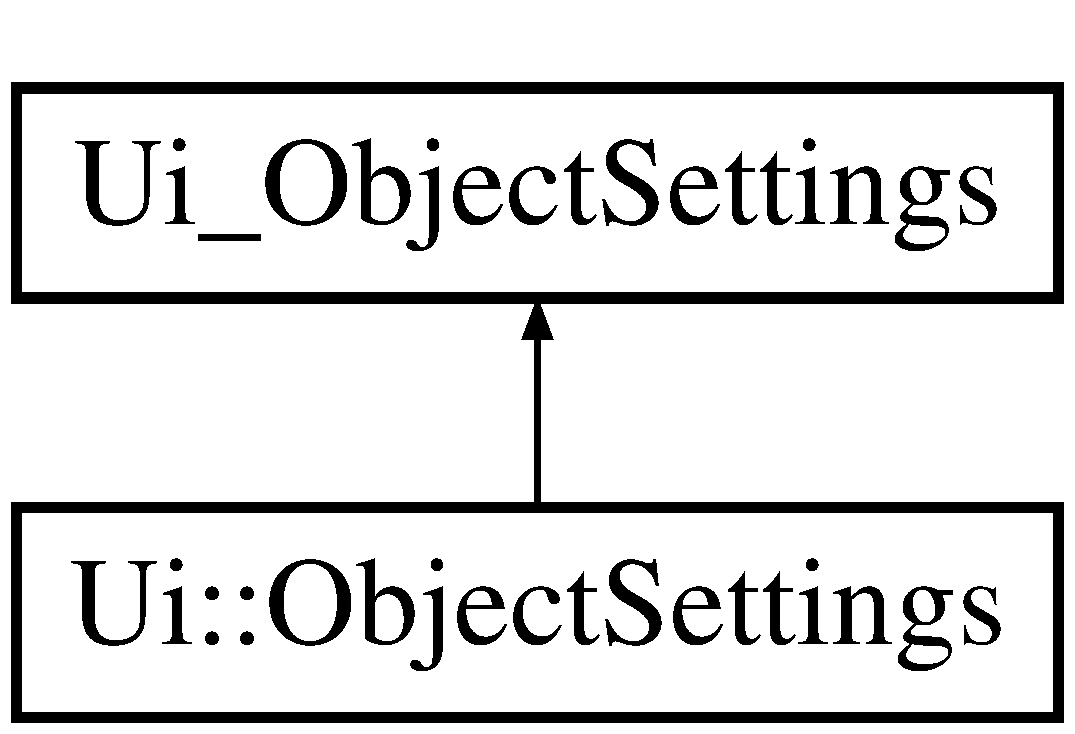
\includegraphics[height=2.000000cm]{class_ui___object_settings}
\end{center}
\end{figure}
\subsection*{Public Member Functions}
\begin{DoxyCompactItemize}
\item 
void \hyperlink{class_ui___object_settings_a9f6ddc78b023afd31f9ee2bb18d3167d}{setup\+Ui} (Q\+Widget $\ast$\hyperlink{class_object_settings}{Object\+Settings})
\item 
void \hyperlink{class_ui___object_settings_a412f3bf2df2d7bbcc4e67bf038566aaa}{retranslate\+Ui} (Q\+Widget $\ast$\hyperlink{class_object_settings}{Object\+Settings})
\end{DoxyCompactItemize}
\subsection*{Public Attributes}
\begin{DoxyCompactItemize}
\item 
Q\+H\+Box\+Layout $\ast$ \hyperlink{class_ui___object_settings_a17d0e29ba40f17b5b637e2954d99f570}{horizontal\+Layout}
\item 
Q\+Group\+Box $\ast$ \hyperlink{class_ui___object_settings_a67cc69d051ed2f4f4e87c0c6036206f3}{Name}
\item 
Q\+V\+Box\+Layout $\ast$ \hyperlink{class_ui___object_settings_a144f8a5ac696bb4e37a59ef120979f9c}{vertical\+Layout}
\item 
Q\+Line\+Edit $\ast$ \hyperlink{class_ui___object_settings_af08ab8f78ce1dd569c6c82635086fadc}{le\+\_\+object\+Name}
\item 
Q\+Group\+Box $\ast$ \hyperlink{class_ui___object_settings_ab73a086c80ad3ff9a53a6aefad85c638}{group\+Box}
\item 
Q\+H\+Box\+Layout $\ast$ \hyperlink{class_ui___object_settings_a1d861c576f62b410578b647f5a817349}{horizontal\+Layout\+\_\+2}
\item 
Q\+Dial $\ast$ \hyperlink{class_ui___object_settings_a824088c070ce22d771e63f62226e179f}{dial}
\item 
Q\+Group\+Box $\ast$ \hyperlink{class_ui___object_settings_a51ffb8d6ab112c3aa5ffa5389084f1f2}{group\+Box\+\_\+2}
\item 
Q\+V\+Box\+Layout $\ast$ \hyperlink{class_ui___object_settings_aadf65497907ac8aca787add49f46a20d}{vertical\+Layout\+\_\+3}
\item 
Q\+Push\+Button $\ast$ \hyperlink{class_ui___object_settings_ac57e5762b345fd94aaca1a09a03ccb73}{push\+Button}
\item 
Q\+Push\+Button $\ast$ \hyperlink{class_ui___object_settings_af39b0ad3b6d8a76b47c82185fc4690f0}{pb\+\_\+delete\+Object}
\end{DoxyCompactItemize}


\subsection{Member Function Documentation}
\mbox{\Hypertarget{class_ui___object_settings_a412f3bf2df2d7bbcc4e67bf038566aaa}\label{class_ui___object_settings_a412f3bf2df2d7bbcc4e67bf038566aaa}} 
\index{Ui\+\_\+\+Object\+Settings@{Ui\+\_\+\+Object\+Settings}!retranslate\+Ui@{retranslate\+Ui}}
\index{retranslate\+Ui@{retranslate\+Ui}!Ui\+\_\+\+Object\+Settings@{Ui\+\_\+\+Object\+Settings}}
\subsubsection{\texorpdfstring{retranslate\+Ui()}{retranslateUi()}}
{\footnotesize\ttfamily void Ui\+\_\+\+Object\+Settings\+::retranslate\+Ui (\begin{DoxyParamCaption}\item[{Q\+Widget $\ast$}]{Object\+Settings }\end{DoxyParamCaption})\hspace{0.3cm}{\ttfamily [inline]}}

\mbox{\Hypertarget{class_ui___object_settings_a9f6ddc78b023afd31f9ee2bb18d3167d}\label{class_ui___object_settings_a9f6ddc78b023afd31f9ee2bb18d3167d}} 
\index{Ui\+\_\+\+Object\+Settings@{Ui\+\_\+\+Object\+Settings}!setup\+Ui@{setup\+Ui}}
\index{setup\+Ui@{setup\+Ui}!Ui\+\_\+\+Object\+Settings@{Ui\+\_\+\+Object\+Settings}}
\subsubsection{\texorpdfstring{setup\+Ui()}{setupUi()}}
{\footnotesize\ttfamily void Ui\+\_\+\+Object\+Settings\+::setup\+Ui (\begin{DoxyParamCaption}\item[{Q\+Widget $\ast$}]{Object\+Settings }\end{DoxyParamCaption})\hspace{0.3cm}{\ttfamily [inline]}}



\subsection{Member Data Documentation}
\mbox{\Hypertarget{class_ui___object_settings_a824088c070ce22d771e63f62226e179f}\label{class_ui___object_settings_a824088c070ce22d771e63f62226e179f}} 
\index{Ui\+\_\+\+Object\+Settings@{Ui\+\_\+\+Object\+Settings}!dial@{dial}}
\index{dial@{dial}!Ui\+\_\+\+Object\+Settings@{Ui\+\_\+\+Object\+Settings}}
\subsubsection{\texorpdfstring{dial}{dial}}
{\footnotesize\ttfamily Q\+Dial$\ast$ Ui\+\_\+\+Object\+Settings\+::dial}

\mbox{\Hypertarget{class_ui___object_settings_ab73a086c80ad3ff9a53a6aefad85c638}\label{class_ui___object_settings_ab73a086c80ad3ff9a53a6aefad85c638}} 
\index{Ui\+\_\+\+Object\+Settings@{Ui\+\_\+\+Object\+Settings}!group\+Box@{group\+Box}}
\index{group\+Box@{group\+Box}!Ui\+\_\+\+Object\+Settings@{Ui\+\_\+\+Object\+Settings}}
\subsubsection{\texorpdfstring{group\+Box}{groupBox}}
{\footnotesize\ttfamily Q\+Group\+Box$\ast$ Ui\+\_\+\+Object\+Settings\+::group\+Box}

\mbox{\Hypertarget{class_ui___object_settings_a51ffb8d6ab112c3aa5ffa5389084f1f2}\label{class_ui___object_settings_a51ffb8d6ab112c3aa5ffa5389084f1f2}} 
\index{Ui\+\_\+\+Object\+Settings@{Ui\+\_\+\+Object\+Settings}!group\+Box\+\_\+2@{group\+Box\+\_\+2}}
\index{group\+Box\+\_\+2@{group\+Box\+\_\+2}!Ui\+\_\+\+Object\+Settings@{Ui\+\_\+\+Object\+Settings}}
\subsubsection{\texorpdfstring{group\+Box\+\_\+2}{groupBox\_2}}
{\footnotesize\ttfamily Q\+Group\+Box$\ast$ Ui\+\_\+\+Object\+Settings\+::group\+Box\+\_\+2}

\mbox{\Hypertarget{class_ui___object_settings_a17d0e29ba40f17b5b637e2954d99f570}\label{class_ui___object_settings_a17d0e29ba40f17b5b637e2954d99f570}} 
\index{Ui\+\_\+\+Object\+Settings@{Ui\+\_\+\+Object\+Settings}!horizontal\+Layout@{horizontal\+Layout}}
\index{horizontal\+Layout@{horizontal\+Layout}!Ui\+\_\+\+Object\+Settings@{Ui\+\_\+\+Object\+Settings}}
\subsubsection{\texorpdfstring{horizontal\+Layout}{horizontalLayout}}
{\footnotesize\ttfamily Q\+H\+Box\+Layout$\ast$ Ui\+\_\+\+Object\+Settings\+::horizontal\+Layout}

\mbox{\Hypertarget{class_ui___object_settings_a1d861c576f62b410578b647f5a817349}\label{class_ui___object_settings_a1d861c576f62b410578b647f5a817349}} 
\index{Ui\+\_\+\+Object\+Settings@{Ui\+\_\+\+Object\+Settings}!horizontal\+Layout\+\_\+2@{horizontal\+Layout\+\_\+2}}
\index{horizontal\+Layout\+\_\+2@{horizontal\+Layout\+\_\+2}!Ui\+\_\+\+Object\+Settings@{Ui\+\_\+\+Object\+Settings}}
\subsubsection{\texorpdfstring{horizontal\+Layout\+\_\+2}{horizontalLayout\_2}}
{\footnotesize\ttfamily Q\+H\+Box\+Layout$\ast$ Ui\+\_\+\+Object\+Settings\+::horizontal\+Layout\+\_\+2}

\mbox{\Hypertarget{class_ui___object_settings_af08ab8f78ce1dd569c6c82635086fadc}\label{class_ui___object_settings_af08ab8f78ce1dd569c6c82635086fadc}} 
\index{Ui\+\_\+\+Object\+Settings@{Ui\+\_\+\+Object\+Settings}!le\+\_\+object\+Name@{le\+\_\+object\+Name}}
\index{le\+\_\+object\+Name@{le\+\_\+object\+Name}!Ui\+\_\+\+Object\+Settings@{Ui\+\_\+\+Object\+Settings}}
\subsubsection{\texorpdfstring{le\+\_\+object\+Name}{le\_objectName}}
{\footnotesize\ttfamily Q\+Line\+Edit$\ast$ Ui\+\_\+\+Object\+Settings\+::le\+\_\+object\+Name}

\mbox{\Hypertarget{class_ui___object_settings_a67cc69d051ed2f4f4e87c0c6036206f3}\label{class_ui___object_settings_a67cc69d051ed2f4f4e87c0c6036206f3}} 
\index{Ui\+\_\+\+Object\+Settings@{Ui\+\_\+\+Object\+Settings}!Name@{Name}}
\index{Name@{Name}!Ui\+\_\+\+Object\+Settings@{Ui\+\_\+\+Object\+Settings}}
\subsubsection{\texorpdfstring{Name}{Name}}
{\footnotesize\ttfamily Q\+Group\+Box$\ast$ Ui\+\_\+\+Object\+Settings\+::\+Name}

\mbox{\Hypertarget{class_ui___object_settings_af39b0ad3b6d8a76b47c82185fc4690f0}\label{class_ui___object_settings_af39b0ad3b6d8a76b47c82185fc4690f0}} 
\index{Ui\+\_\+\+Object\+Settings@{Ui\+\_\+\+Object\+Settings}!pb\+\_\+delete\+Object@{pb\+\_\+delete\+Object}}
\index{pb\+\_\+delete\+Object@{pb\+\_\+delete\+Object}!Ui\+\_\+\+Object\+Settings@{Ui\+\_\+\+Object\+Settings}}
\subsubsection{\texorpdfstring{pb\+\_\+delete\+Object}{pb\_deleteObject}}
{\footnotesize\ttfamily Q\+Push\+Button$\ast$ Ui\+\_\+\+Object\+Settings\+::pb\+\_\+delete\+Object}

\mbox{\Hypertarget{class_ui___object_settings_ac57e5762b345fd94aaca1a09a03ccb73}\label{class_ui___object_settings_ac57e5762b345fd94aaca1a09a03ccb73}} 
\index{Ui\+\_\+\+Object\+Settings@{Ui\+\_\+\+Object\+Settings}!push\+Button@{push\+Button}}
\index{push\+Button@{push\+Button}!Ui\+\_\+\+Object\+Settings@{Ui\+\_\+\+Object\+Settings}}
\subsubsection{\texorpdfstring{push\+Button}{pushButton}}
{\footnotesize\ttfamily Q\+Push\+Button$\ast$ Ui\+\_\+\+Object\+Settings\+::push\+Button}

\mbox{\Hypertarget{class_ui___object_settings_a144f8a5ac696bb4e37a59ef120979f9c}\label{class_ui___object_settings_a144f8a5ac696bb4e37a59ef120979f9c}} 
\index{Ui\+\_\+\+Object\+Settings@{Ui\+\_\+\+Object\+Settings}!vertical\+Layout@{vertical\+Layout}}
\index{vertical\+Layout@{vertical\+Layout}!Ui\+\_\+\+Object\+Settings@{Ui\+\_\+\+Object\+Settings}}
\subsubsection{\texorpdfstring{vertical\+Layout}{verticalLayout}}
{\footnotesize\ttfamily Q\+V\+Box\+Layout$\ast$ Ui\+\_\+\+Object\+Settings\+::vertical\+Layout}

\mbox{\Hypertarget{class_ui___object_settings_aadf65497907ac8aca787add49f46a20d}\label{class_ui___object_settings_aadf65497907ac8aca787add49f46a20d}} 
\index{Ui\+\_\+\+Object\+Settings@{Ui\+\_\+\+Object\+Settings}!vertical\+Layout\+\_\+3@{vertical\+Layout\+\_\+3}}
\index{vertical\+Layout\+\_\+3@{vertical\+Layout\+\_\+3}!Ui\+\_\+\+Object\+Settings@{Ui\+\_\+\+Object\+Settings}}
\subsubsection{\texorpdfstring{vertical\+Layout\+\_\+3}{verticalLayout\_3}}
{\footnotesize\ttfamily Q\+V\+Box\+Layout$\ast$ Ui\+\_\+\+Object\+Settings\+::vertical\+Layout\+\_\+3}



The documentation for this class was generated from the following file\+:\begin{DoxyCompactItemize}
\item 
\hyperlink{ui__objectsettings_8h}{ui\+\_\+objectsettings.\+h}\end{DoxyCompactItemize}

\hypertarget{class_ui___tutorial_line_tool}{}\section{Ui\+\_\+\+Tutorial\+Line\+Tool Class Reference}
\label{class_ui___tutorial_line_tool}\index{Ui\+\_\+\+Tutorial\+Line\+Tool@{Ui\+\_\+\+Tutorial\+Line\+Tool}}


{\ttfamily \#include $<$ui\+\_\+tutoriallinetool.\+h$>$}

Inheritance diagram for Ui\+\_\+\+Tutorial\+Line\+Tool\+:\begin{figure}[H]
\begin{center}
\leavevmode
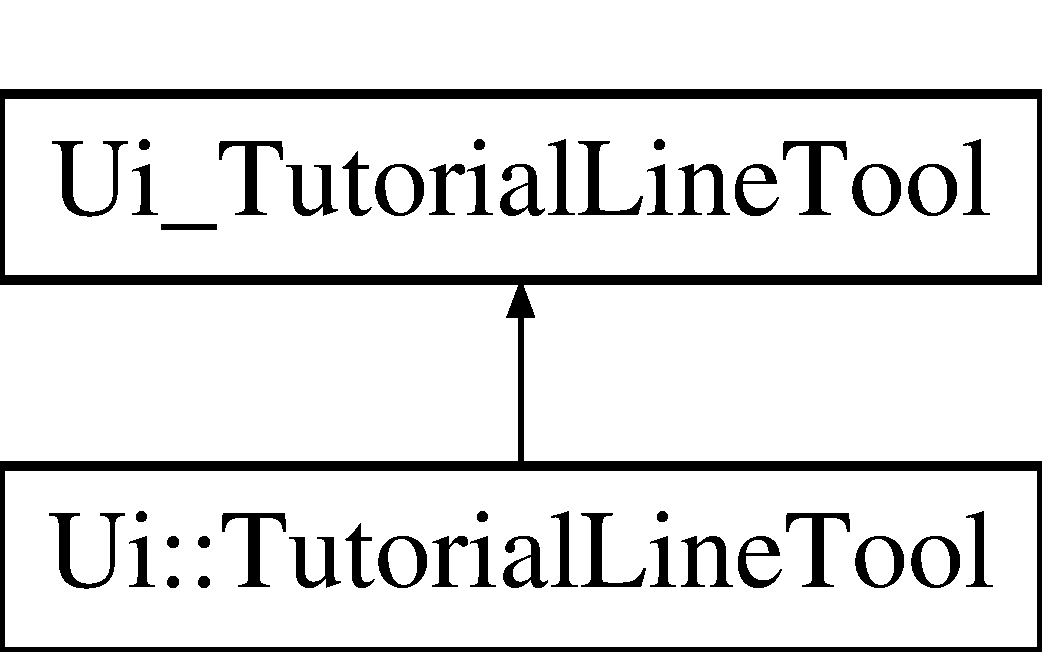
\includegraphics[height=2.000000cm]{class_ui___tutorial_line_tool}
\end{center}
\end{figure}
\subsection*{Public Member Functions}
\begin{DoxyCompactItemize}
\item 
void \hyperlink{class_ui___tutorial_line_tool_a93d6e45a92b3913055a1237d7ca9a572}{setup\+Ui} (Q\+Dialog $\ast$\hyperlink{class_tutorial_line_tool}{Tutorial\+Line\+Tool})
\item 
void \hyperlink{class_ui___tutorial_line_tool_a44f97272d6c2a19a07624b62c707dc01}{retranslate\+Ui} (Q\+Dialog $\ast$\hyperlink{class_tutorial_line_tool}{Tutorial\+Line\+Tool})
\end{DoxyCompactItemize}
\subsection*{Public Attributes}
\begin{DoxyCompactItemize}
\item 
Q\+Grid\+Layout $\ast$ \hyperlink{class_ui___tutorial_line_tool_ae8278b4d4acc9b26ff5e41896018dbb7}{grid\+Layout}
\item 
Q\+Group\+Box $\ast$ \hyperlink{class_ui___tutorial_line_tool_aac7a297d62be49df306ca51485db55b9}{group\+Box\+\_\+2}
\item 
Q\+Grid\+Layout $\ast$ \hyperlink{class_ui___tutorial_line_tool_a5b19cfb803820e0bf6dbbd5049399b14}{grid\+Layout\+\_\+3}
\item 
Q\+Widget $\ast$ \hyperlink{class_ui___tutorial_line_tool_aa75a71bc65f21bf083197dd534bcf95e}{widget\+\_\+2}
\item 
Q\+Label $\ast$ \hyperlink{class_ui___tutorial_line_tool_aef3b51804ab6c5c4147549621a6d3f44}{label\+\_\+4}
\item 
Q\+Label $\ast$ \hyperlink{class_ui___tutorial_line_tool_adc1777cbeaea98dd945f1981cc55d9a0}{label\+\_\+3}
\item 
Q\+Widget $\ast$ \hyperlink{class_ui___tutorial_line_tool_a23abf750d7407913b339fc3c355a0f39}{widget}
\item 
Q\+Group\+Box $\ast$ \hyperlink{class_ui___tutorial_line_tool_a08f56eac86b481508d628df6e495d90f}{group\+Box\+\_\+3}
\item 
Q\+Grid\+Layout $\ast$ \hyperlink{class_ui___tutorial_line_tool_a15a88ba2a2034f5f9d45dec12d81e2df}{grid\+Layout\+\_\+4}
\item 
Q\+Push\+Button $\ast$ \hyperlink{class_ui___tutorial_line_tool_a5edea9a3f263fbcc561466740cf232cb}{push\+Button\+\_\+3}
\item 
Q\+Push\+Button $\ast$ \hyperlink{class_ui___tutorial_line_tool_a2c8560f352b1a0a838d1e30d4044ecc3}{push\+Button\+\_\+2}
\item 
Q\+Label $\ast$ \hyperlink{class_ui___tutorial_line_tool_aa6d4e0591eb37e4dbbe2071a6d5f9326}{label\+\_\+5}
\item 
Q\+Label $\ast$ \hyperlink{class_ui___tutorial_line_tool_a3618bc42bbee059ab46d27fdeebe7286}{label\+\_\+6}
\item 
Q\+Group\+Box $\ast$ \hyperlink{class_ui___tutorial_line_tool_ae5c609a78890875a99406c60b2fcd54c}{group\+Box}
\item 
Q\+Grid\+Layout $\ast$ \hyperlink{class_ui___tutorial_line_tool_a6e8d84fec289339b46535d2f360b24ed}{grid\+Layout\+\_\+2}
\item 
Q\+Push\+Button $\ast$ \hyperlink{class_ui___tutorial_line_tool_a8018d808b53875c8e0ea20fe19a1228f}{push\+Button}
\item 
Q\+Label $\ast$ \hyperlink{class_ui___tutorial_line_tool_a7c0e201a32afbf07d48fba3bfd249f6c}{label}
\item 
Q\+Label $\ast$ \hyperlink{class_ui___tutorial_line_tool_a0b3e484c78e9e554d586c606660942c4}{label\+\_\+2}
\item 
Q\+Dialog\+Button\+Box $\ast$ \hyperlink{class_ui___tutorial_line_tool_a92071438258241a995532410beff096e}{button\+Box}
\end{DoxyCompactItemize}


\subsection{Member Function Documentation}
\mbox{\Hypertarget{class_ui___tutorial_line_tool_a44f97272d6c2a19a07624b62c707dc01}\label{class_ui___tutorial_line_tool_a44f97272d6c2a19a07624b62c707dc01}} 
\index{Ui\+\_\+\+Tutorial\+Line\+Tool@{Ui\+\_\+\+Tutorial\+Line\+Tool}!retranslate\+Ui@{retranslate\+Ui}}
\index{retranslate\+Ui@{retranslate\+Ui}!Ui\+\_\+\+Tutorial\+Line\+Tool@{Ui\+\_\+\+Tutorial\+Line\+Tool}}
\subsubsection{\texorpdfstring{retranslate\+Ui()}{retranslateUi()}}
{\footnotesize\ttfamily void Ui\+\_\+\+Tutorial\+Line\+Tool\+::retranslate\+Ui (\begin{DoxyParamCaption}\item[{Q\+Dialog $\ast$}]{Tutorial\+Line\+Tool }\end{DoxyParamCaption})\hspace{0.3cm}{\ttfamily [inline]}}

\mbox{\Hypertarget{class_ui___tutorial_line_tool_a93d6e45a92b3913055a1237d7ca9a572}\label{class_ui___tutorial_line_tool_a93d6e45a92b3913055a1237d7ca9a572}} 
\index{Ui\+\_\+\+Tutorial\+Line\+Tool@{Ui\+\_\+\+Tutorial\+Line\+Tool}!setup\+Ui@{setup\+Ui}}
\index{setup\+Ui@{setup\+Ui}!Ui\+\_\+\+Tutorial\+Line\+Tool@{Ui\+\_\+\+Tutorial\+Line\+Tool}}
\subsubsection{\texorpdfstring{setup\+Ui()}{setupUi()}}
{\footnotesize\ttfamily void Ui\+\_\+\+Tutorial\+Line\+Tool\+::setup\+Ui (\begin{DoxyParamCaption}\item[{Q\+Dialog $\ast$}]{Tutorial\+Line\+Tool }\end{DoxyParamCaption})\hspace{0.3cm}{\ttfamily [inline]}}



\subsection{Member Data Documentation}
\mbox{\Hypertarget{class_ui___tutorial_line_tool_a92071438258241a995532410beff096e}\label{class_ui___tutorial_line_tool_a92071438258241a995532410beff096e}} 
\index{Ui\+\_\+\+Tutorial\+Line\+Tool@{Ui\+\_\+\+Tutorial\+Line\+Tool}!button\+Box@{button\+Box}}
\index{button\+Box@{button\+Box}!Ui\+\_\+\+Tutorial\+Line\+Tool@{Ui\+\_\+\+Tutorial\+Line\+Tool}}
\subsubsection{\texorpdfstring{button\+Box}{buttonBox}}
{\footnotesize\ttfamily Q\+Dialog\+Button\+Box$\ast$ Ui\+\_\+\+Tutorial\+Line\+Tool\+::button\+Box}

\mbox{\Hypertarget{class_ui___tutorial_line_tool_ae8278b4d4acc9b26ff5e41896018dbb7}\label{class_ui___tutorial_line_tool_ae8278b4d4acc9b26ff5e41896018dbb7}} 
\index{Ui\+\_\+\+Tutorial\+Line\+Tool@{Ui\+\_\+\+Tutorial\+Line\+Tool}!grid\+Layout@{grid\+Layout}}
\index{grid\+Layout@{grid\+Layout}!Ui\+\_\+\+Tutorial\+Line\+Tool@{Ui\+\_\+\+Tutorial\+Line\+Tool}}
\subsubsection{\texorpdfstring{grid\+Layout}{gridLayout}}
{\footnotesize\ttfamily Q\+Grid\+Layout$\ast$ Ui\+\_\+\+Tutorial\+Line\+Tool\+::grid\+Layout}

\mbox{\Hypertarget{class_ui___tutorial_line_tool_a6e8d84fec289339b46535d2f360b24ed}\label{class_ui___tutorial_line_tool_a6e8d84fec289339b46535d2f360b24ed}} 
\index{Ui\+\_\+\+Tutorial\+Line\+Tool@{Ui\+\_\+\+Tutorial\+Line\+Tool}!grid\+Layout\+\_\+2@{grid\+Layout\+\_\+2}}
\index{grid\+Layout\+\_\+2@{grid\+Layout\+\_\+2}!Ui\+\_\+\+Tutorial\+Line\+Tool@{Ui\+\_\+\+Tutorial\+Line\+Tool}}
\subsubsection{\texorpdfstring{grid\+Layout\+\_\+2}{gridLayout\_2}}
{\footnotesize\ttfamily Q\+Grid\+Layout$\ast$ Ui\+\_\+\+Tutorial\+Line\+Tool\+::grid\+Layout\+\_\+2}

\mbox{\Hypertarget{class_ui___tutorial_line_tool_a5b19cfb803820e0bf6dbbd5049399b14}\label{class_ui___tutorial_line_tool_a5b19cfb803820e0bf6dbbd5049399b14}} 
\index{Ui\+\_\+\+Tutorial\+Line\+Tool@{Ui\+\_\+\+Tutorial\+Line\+Tool}!grid\+Layout\+\_\+3@{grid\+Layout\+\_\+3}}
\index{grid\+Layout\+\_\+3@{grid\+Layout\+\_\+3}!Ui\+\_\+\+Tutorial\+Line\+Tool@{Ui\+\_\+\+Tutorial\+Line\+Tool}}
\subsubsection{\texorpdfstring{grid\+Layout\+\_\+3}{gridLayout\_3}}
{\footnotesize\ttfamily Q\+Grid\+Layout$\ast$ Ui\+\_\+\+Tutorial\+Line\+Tool\+::grid\+Layout\+\_\+3}

\mbox{\Hypertarget{class_ui___tutorial_line_tool_a15a88ba2a2034f5f9d45dec12d81e2df}\label{class_ui___tutorial_line_tool_a15a88ba2a2034f5f9d45dec12d81e2df}} 
\index{Ui\+\_\+\+Tutorial\+Line\+Tool@{Ui\+\_\+\+Tutorial\+Line\+Tool}!grid\+Layout\+\_\+4@{grid\+Layout\+\_\+4}}
\index{grid\+Layout\+\_\+4@{grid\+Layout\+\_\+4}!Ui\+\_\+\+Tutorial\+Line\+Tool@{Ui\+\_\+\+Tutorial\+Line\+Tool}}
\subsubsection{\texorpdfstring{grid\+Layout\+\_\+4}{gridLayout\_4}}
{\footnotesize\ttfamily Q\+Grid\+Layout$\ast$ Ui\+\_\+\+Tutorial\+Line\+Tool\+::grid\+Layout\+\_\+4}

\mbox{\Hypertarget{class_ui___tutorial_line_tool_ae5c609a78890875a99406c60b2fcd54c}\label{class_ui___tutorial_line_tool_ae5c609a78890875a99406c60b2fcd54c}} 
\index{Ui\+\_\+\+Tutorial\+Line\+Tool@{Ui\+\_\+\+Tutorial\+Line\+Tool}!group\+Box@{group\+Box}}
\index{group\+Box@{group\+Box}!Ui\+\_\+\+Tutorial\+Line\+Tool@{Ui\+\_\+\+Tutorial\+Line\+Tool}}
\subsubsection{\texorpdfstring{group\+Box}{groupBox}}
{\footnotesize\ttfamily Q\+Group\+Box$\ast$ Ui\+\_\+\+Tutorial\+Line\+Tool\+::group\+Box}

\mbox{\Hypertarget{class_ui___tutorial_line_tool_aac7a297d62be49df306ca51485db55b9}\label{class_ui___tutorial_line_tool_aac7a297d62be49df306ca51485db55b9}} 
\index{Ui\+\_\+\+Tutorial\+Line\+Tool@{Ui\+\_\+\+Tutorial\+Line\+Tool}!group\+Box\+\_\+2@{group\+Box\+\_\+2}}
\index{group\+Box\+\_\+2@{group\+Box\+\_\+2}!Ui\+\_\+\+Tutorial\+Line\+Tool@{Ui\+\_\+\+Tutorial\+Line\+Tool}}
\subsubsection{\texorpdfstring{group\+Box\+\_\+2}{groupBox\_2}}
{\footnotesize\ttfamily Q\+Group\+Box$\ast$ Ui\+\_\+\+Tutorial\+Line\+Tool\+::group\+Box\+\_\+2}

\mbox{\Hypertarget{class_ui___tutorial_line_tool_a08f56eac86b481508d628df6e495d90f}\label{class_ui___tutorial_line_tool_a08f56eac86b481508d628df6e495d90f}} 
\index{Ui\+\_\+\+Tutorial\+Line\+Tool@{Ui\+\_\+\+Tutorial\+Line\+Tool}!group\+Box\+\_\+3@{group\+Box\+\_\+3}}
\index{group\+Box\+\_\+3@{group\+Box\+\_\+3}!Ui\+\_\+\+Tutorial\+Line\+Tool@{Ui\+\_\+\+Tutorial\+Line\+Tool}}
\subsubsection{\texorpdfstring{group\+Box\+\_\+3}{groupBox\_3}}
{\footnotesize\ttfamily Q\+Group\+Box$\ast$ Ui\+\_\+\+Tutorial\+Line\+Tool\+::group\+Box\+\_\+3}

\mbox{\Hypertarget{class_ui___tutorial_line_tool_a7c0e201a32afbf07d48fba3bfd249f6c}\label{class_ui___tutorial_line_tool_a7c0e201a32afbf07d48fba3bfd249f6c}} 
\index{Ui\+\_\+\+Tutorial\+Line\+Tool@{Ui\+\_\+\+Tutorial\+Line\+Tool}!label@{label}}
\index{label@{label}!Ui\+\_\+\+Tutorial\+Line\+Tool@{Ui\+\_\+\+Tutorial\+Line\+Tool}}
\subsubsection{\texorpdfstring{label}{label}}
{\footnotesize\ttfamily Q\+Label$\ast$ Ui\+\_\+\+Tutorial\+Line\+Tool\+::label}

\mbox{\Hypertarget{class_ui___tutorial_line_tool_a0b3e484c78e9e554d586c606660942c4}\label{class_ui___tutorial_line_tool_a0b3e484c78e9e554d586c606660942c4}} 
\index{Ui\+\_\+\+Tutorial\+Line\+Tool@{Ui\+\_\+\+Tutorial\+Line\+Tool}!label\+\_\+2@{label\+\_\+2}}
\index{label\+\_\+2@{label\+\_\+2}!Ui\+\_\+\+Tutorial\+Line\+Tool@{Ui\+\_\+\+Tutorial\+Line\+Tool}}
\subsubsection{\texorpdfstring{label\+\_\+2}{label\_2}}
{\footnotesize\ttfamily Q\+Label$\ast$ Ui\+\_\+\+Tutorial\+Line\+Tool\+::label\+\_\+2}

\mbox{\Hypertarget{class_ui___tutorial_line_tool_adc1777cbeaea98dd945f1981cc55d9a0}\label{class_ui___tutorial_line_tool_adc1777cbeaea98dd945f1981cc55d9a0}} 
\index{Ui\+\_\+\+Tutorial\+Line\+Tool@{Ui\+\_\+\+Tutorial\+Line\+Tool}!label\+\_\+3@{label\+\_\+3}}
\index{label\+\_\+3@{label\+\_\+3}!Ui\+\_\+\+Tutorial\+Line\+Tool@{Ui\+\_\+\+Tutorial\+Line\+Tool}}
\subsubsection{\texorpdfstring{label\+\_\+3}{label\_3}}
{\footnotesize\ttfamily Q\+Label$\ast$ Ui\+\_\+\+Tutorial\+Line\+Tool\+::label\+\_\+3}

\mbox{\Hypertarget{class_ui___tutorial_line_tool_aef3b51804ab6c5c4147549621a6d3f44}\label{class_ui___tutorial_line_tool_aef3b51804ab6c5c4147549621a6d3f44}} 
\index{Ui\+\_\+\+Tutorial\+Line\+Tool@{Ui\+\_\+\+Tutorial\+Line\+Tool}!label\+\_\+4@{label\+\_\+4}}
\index{label\+\_\+4@{label\+\_\+4}!Ui\+\_\+\+Tutorial\+Line\+Tool@{Ui\+\_\+\+Tutorial\+Line\+Tool}}
\subsubsection{\texorpdfstring{label\+\_\+4}{label\_4}}
{\footnotesize\ttfamily Q\+Label$\ast$ Ui\+\_\+\+Tutorial\+Line\+Tool\+::label\+\_\+4}

\mbox{\Hypertarget{class_ui___tutorial_line_tool_aa6d4e0591eb37e4dbbe2071a6d5f9326}\label{class_ui___tutorial_line_tool_aa6d4e0591eb37e4dbbe2071a6d5f9326}} 
\index{Ui\+\_\+\+Tutorial\+Line\+Tool@{Ui\+\_\+\+Tutorial\+Line\+Tool}!label\+\_\+5@{label\+\_\+5}}
\index{label\+\_\+5@{label\+\_\+5}!Ui\+\_\+\+Tutorial\+Line\+Tool@{Ui\+\_\+\+Tutorial\+Line\+Tool}}
\subsubsection{\texorpdfstring{label\+\_\+5}{label\_5}}
{\footnotesize\ttfamily Q\+Label$\ast$ Ui\+\_\+\+Tutorial\+Line\+Tool\+::label\+\_\+5}

\mbox{\Hypertarget{class_ui___tutorial_line_tool_a3618bc42bbee059ab46d27fdeebe7286}\label{class_ui___tutorial_line_tool_a3618bc42bbee059ab46d27fdeebe7286}} 
\index{Ui\+\_\+\+Tutorial\+Line\+Tool@{Ui\+\_\+\+Tutorial\+Line\+Tool}!label\+\_\+6@{label\+\_\+6}}
\index{label\+\_\+6@{label\+\_\+6}!Ui\+\_\+\+Tutorial\+Line\+Tool@{Ui\+\_\+\+Tutorial\+Line\+Tool}}
\subsubsection{\texorpdfstring{label\+\_\+6}{label\_6}}
{\footnotesize\ttfamily Q\+Label$\ast$ Ui\+\_\+\+Tutorial\+Line\+Tool\+::label\+\_\+6}

\mbox{\Hypertarget{class_ui___tutorial_line_tool_a8018d808b53875c8e0ea20fe19a1228f}\label{class_ui___tutorial_line_tool_a8018d808b53875c8e0ea20fe19a1228f}} 
\index{Ui\+\_\+\+Tutorial\+Line\+Tool@{Ui\+\_\+\+Tutorial\+Line\+Tool}!push\+Button@{push\+Button}}
\index{push\+Button@{push\+Button}!Ui\+\_\+\+Tutorial\+Line\+Tool@{Ui\+\_\+\+Tutorial\+Line\+Tool}}
\subsubsection{\texorpdfstring{push\+Button}{pushButton}}
{\footnotesize\ttfamily Q\+Push\+Button$\ast$ Ui\+\_\+\+Tutorial\+Line\+Tool\+::push\+Button}

\mbox{\Hypertarget{class_ui___tutorial_line_tool_a2c8560f352b1a0a838d1e30d4044ecc3}\label{class_ui___tutorial_line_tool_a2c8560f352b1a0a838d1e30d4044ecc3}} 
\index{Ui\+\_\+\+Tutorial\+Line\+Tool@{Ui\+\_\+\+Tutorial\+Line\+Tool}!push\+Button\+\_\+2@{push\+Button\+\_\+2}}
\index{push\+Button\+\_\+2@{push\+Button\+\_\+2}!Ui\+\_\+\+Tutorial\+Line\+Tool@{Ui\+\_\+\+Tutorial\+Line\+Tool}}
\subsubsection{\texorpdfstring{push\+Button\+\_\+2}{pushButton\_2}}
{\footnotesize\ttfamily Q\+Push\+Button$\ast$ Ui\+\_\+\+Tutorial\+Line\+Tool\+::push\+Button\+\_\+2}

\mbox{\Hypertarget{class_ui___tutorial_line_tool_a5edea9a3f263fbcc561466740cf232cb}\label{class_ui___tutorial_line_tool_a5edea9a3f263fbcc561466740cf232cb}} 
\index{Ui\+\_\+\+Tutorial\+Line\+Tool@{Ui\+\_\+\+Tutorial\+Line\+Tool}!push\+Button\+\_\+3@{push\+Button\+\_\+3}}
\index{push\+Button\+\_\+3@{push\+Button\+\_\+3}!Ui\+\_\+\+Tutorial\+Line\+Tool@{Ui\+\_\+\+Tutorial\+Line\+Tool}}
\subsubsection{\texorpdfstring{push\+Button\+\_\+3}{pushButton\_3}}
{\footnotesize\ttfamily Q\+Push\+Button$\ast$ Ui\+\_\+\+Tutorial\+Line\+Tool\+::push\+Button\+\_\+3}

\mbox{\Hypertarget{class_ui___tutorial_line_tool_a23abf750d7407913b339fc3c355a0f39}\label{class_ui___tutorial_line_tool_a23abf750d7407913b339fc3c355a0f39}} 
\index{Ui\+\_\+\+Tutorial\+Line\+Tool@{Ui\+\_\+\+Tutorial\+Line\+Tool}!widget@{widget}}
\index{widget@{widget}!Ui\+\_\+\+Tutorial\+Line\+Tool@{Ui\+\_\+\+Tutorial\+Line\+Tool}}
\subsubsection{\texorpdfstring{widget}{widget}}
{\footnotesize\ttfamily Q\+Widget$\ast$ Ui\+\_\+\+Tutorial\+Line\+Tool\+::widget}

\mbox{\Hypertarget{class_ui___tutorial_line_tool_aa75a71bc65f21bf083197dd534bcf95e}\label{class_ui___tutorial_line_tool_aa75a71bc65f21bf083197dd534bcf95e}} 
\index{Ui\+\_\+\+Tutorial\+Line\+Tool@{Ui\+\_\+\+Tutorial\+Line\+Tool}!widget\+\_\+2@{widget\+\_\+2}}
\index{widget\+\_\+2@{widget\+\_\+2}!Ui\+\_\+\+Tutorial\+Line\+Tool@{Ui\+\_\+\+Tutorial\+Line\+Tool}}
\subsubsection{\texorpdfstring{widget\+\_\+2}{widget\_2}}
{\footnotesize\ttfamily Q\+Widget$\ast$ Ui\+\_\+\+Tutorial\+Line\+Tool\+::widget\+\_\+2}



The documentation for this class was generated from the following file\+:\begin{DoxyCompactItemize}
\item 
\hyperlink{ui__tutoriallinetool_8h}{ui\+\_\+tutoriallinetool.\+h}\end{DoxyCompactItemize}

\hypertarget{class_ui___welcome_dialog}{}\section{Ui\+\_\+\+Welcome\+Dialog Class Reference}
\label{class_ui___welcome_dialog}\index{Ui\+\_\+\+Welcome\+Dialog@{Ui\+\_\+\+Welcome\+Dialog}}


{\ttfamily \#include $<$ui\+\_\+welcomedialog.\+h$>$}

Inheritance diagram for Ui\+\_\+\+Welcome\+Dialog\+:\begin{figure}[H]
\begin{center}
\leavevmode
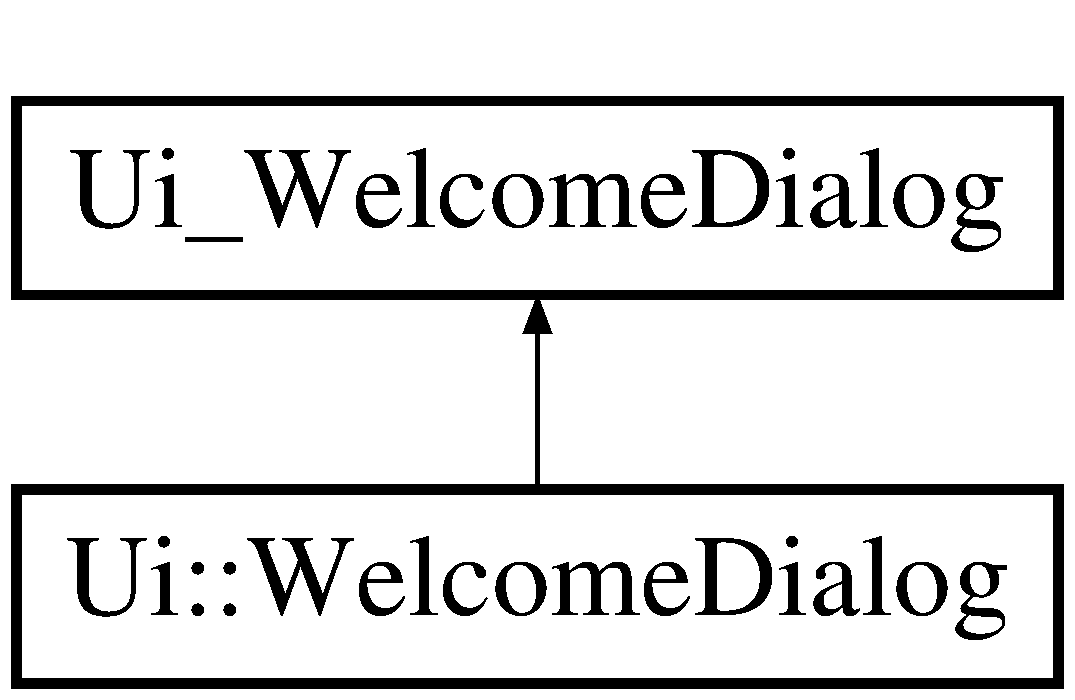
\includegraphics[height=2.000000cm]{class_ui___welcome_dialog}
\end{center}
\end{figure}
\subsection*{Public Member Functions}
\begin{DoxyCompactItemize}
\item 
void \hyperlink{class_ui___welcome_dialog_a423d87674cd389d9780493c4e69d3d9a}{setup\+Ui} (Q\+Dialog $\ast$\hyperlink{class_welcome_dialog}{Welcome\+Dialog})
\item 
void \hyperlink{class_ui___welcome_dialog_a6a7b7092cef38c1fe68a40809e4caeb0}{retranslate\+Ui} (Q\+Dialog $\ast$\hyperlink{class_welcome_dialog}{Welcome\+Dialog})
\end{DoxyCompactItemize}
\subsection*{Public Attributes}
\begin{DoxyCompactItemize}
\item 
Q\+Grid\+Layout $\ast$ \hyperlink{class_ui___welcome_dialog_ad7da50ea9c67116aa89f5b4e31d10724}{grid\+Layout}
\item 
Q\+Dialog\+Button\+Box $\ast$ \hyperlink{class_ui___welcome_dialog_a6f6ead35c5b555fb6daa786b336c7257}{button\+Box}
\item 
Q\+Label $\ast$ \hyperlink{class_ui___welcome_dialog_a26c3765f036a65966735849dfb9debfd}{label}
\item 
Q\+Widget $\ast$ \hyperlink{class_ui___welcome_dialog_a1f3c7de8c4595581eaa129e8d0642d2e}{widget}
\item 
Q\+Spacer\+Item $\ast$ \hyperlink{class_ui___welcome_dialog_a5d8f10bc52bc95ae0f9fdb0f40dd8242}{vertical\+Spacer}
\end{DoxyCompactItemize}


\subsection{Member Function Documentation}
\mbox{\Hypertarget{class_ui___welcome_dialog_a6a7b7092cef38c1fe68a40809e4caeb0}\label{class_ui___welcome_dialog_a6a7b7092cef38c1fe68a40809e4caeb0}} 
\index{Ui\+\_\+\+Welcome\+Dialog@{Ui\+\_\+\+Welcome\+Dialog}!retranslate\+Ui@{retranslate\+Ui}}
\index{retranslate\+Ui@{retranslate\+Ui}!Ui\+\_\+\+Welcome\+Dialog@{Ui\+\_\+\+Welcome\+Dialog}}
\subsubsection{\texorpdfstring{retranslate\+Ui()}{retranslateUi()}}
{\footnotesize\ttfamily void Ui\+\_\+\+Welcome\+Dialog\+::retranslate\+Ui (\begin{DoxyParamCaption}\item[{Q\+Dialog $\ast$}]{Welcome\+Dialog }\end{DoxyParamCaption})\hspace{0.3cm}{\ttfamily [inline]}}

\mbox{\Hypertarget{class_ui___welcome_dialog_a423d87674cd389d9780493c4e69d3d9a}\label{class_ui___welcome_dialog_a423d87674cd389d9780493c4e69d3d9a}} 
\index{Ui\+\_\+\+Welcome\+Dialog@{Ui\+\_\+\+Welcome\+Dialog}!setup\+Ui@{setup\+Ui}}
\index{setup\+Ui@{setup\+Ui}!Ui\+\_\+\+Welcome\+Dialog@{Ui\+\_\+\+Welcome\+Dialog}}
\subsubsection{\texorpdfstring{setup\+Ui()}{setupUi()}}
{\footnotesize\ttfamily void Ui\+\_\+\+Welcome\+Dialog\+::setup\+Ui (\begin{DoxyParamCaption}\item[{Q\+Dialog $\ast$}]{Welcome\+Dialog }\end{DoxyParamCaption})\hspace{0.3cm}{\ttfamily [inline]}}



\subsection{Member Data Documentation}
\mbox{\Hypertarget{class_ui___welcome_dialog_a6f6ead35c5b555fb6daa786b336c7257}\label{class_ui___welcome_dialog_a6f6ead35c5b555fb6daa786b336c7257}} 
\index{Ui\+\_\+\+Welcome\+Dialog@{Ui\+\_\+\+Welcome\+Dialog}!button\+Box@{button\+Box}}
\index{button\+Box@{button\+Box}!Ui\+\_\+\+Welcome\+Dialog@{Ui\+\_\+\+Welcome\+Dialog}}
\subsubsection{\texorpdfstring{button\+Box}{buttonBox}}
{\footnotesize\ttfamily Q\+Dialog\+Button\+Box$\ast$ Ui\+\_\+\+Welcome\+Dialog\+::button\+Box}

\mbox{\Hypertarget{class_ui___welcome_dialog_ad7da50ea9c67116aa89f5b4e31d10724}\label{class_ui___welcome_dialog_ad7da50ea9c67116aa89f5b4e31d10724}} 
\index{Ui\+\_\+\+Welcome\+Dialog@{Ui\+\_\+\+Welcome\+Dialog}!grid\+Layout@{grid\+Layout}}
\index{grid\+Layout@{grid\+Layout}!Ui\+\_\+\+Welcome\+Dialog@{Ui\+\_\+\+Welcome\+Dialog}}
\subsubsection{\texorpdfstring{grid\+Layout}{gridLayout}}
{\footnotesize\ttfamily Q\+Grid\+Layout$\ast$ Ui\+\_\+\+Welcome\+Dialog\+::grid\+Layout}

\mbox{\Hypertarget{class_ui___welcome_dialog_a26c3765f036a65966735849dfb9debfd}\label{class_ui___welcome_dialog_a26c3765f036a65966735849dfb9debfd}} 
\index{Ui\+\_\+\+Welcome\+Dialog@{Ui\+\_\+\+Welcome\+Dialog}!label@{label}}
\index{label@{label}!Ui\+\_\+\+Welcome\+Dialog@{Ui\+\_\+\+Welcome\+Dialog}}
\subsubsection{\texorpdfstring{label}{label}}
{\footnotesize\ttfamily Q\+Label$\ast$ Ui\+\_\+\+Welcome\+Dialog\+::label}

\mbox{\Hypertarget{class_ui___welcome_dialog_a5d8f10bc52bc95ae0f9fdb0f40dd8242}\label{class_ui___welcome_dialog_a5d8f10bc52bc95ae0f9fdb0f40dd8242}} 
\index{Ui\+\_\+\+Welcome\+Dialog@{Ui\+\_\+\+Welcome\+Dialog}!vertical\+Spacer@{vertical\+Spacer}}
\index{vertical\+Spacer@{vertical\+Spacer}!Ui\+\_\+\+Welcome\+Dialog@{Ui\+\_\+\+Welcome\+Dialog}}
\subsubsection{\texorpdfstring{vertical\+Spacer}{verticalSpacer}}
{\footnotesize\ttfamily Q\+Spacer\+Item$\ast$ Ui\+\_\+\+Welcome\+Dialog\+::vertical\+Spacer}

\mbox{\Hypertarget{class_ui___welcome_dialog_a1f3c7de8c4595581eaa129e8d0642d2e}\label{class_ui___welcome_dialog_a1f3c7de8c4595581eaa129e8d0642d2e}} 
\index{Ui\+\_\+\+Welcome\+Dialog@{Ui\+\_\+\+Welcome\+Dialog}!widget@{widget}}
\index{widget@{widget}!Ui\+\_\+\+Welcome\+Dialog@{Ui\+\_\+\+Welcome\+Dialog}}
\subsubsection{\texorpdfstring{widget}{widget}}
{\footnotesize\ttfamily Q\+Widget$\ast$ Ui\+\_\+\+Welcome\+Dialog\+::widget}



The documentation for this class was generated from the following file\+:\begin{DoxyCompactItemize}
\item 
\hyperlink{ui__welcomedialog_8h}{ui\+\_\+welcomedialog.\+h}\end{DoxyCompactItemize}

\hypertarget{class_ui_1_1_welcome_dialog}{}\section{Ui\+:\+:Welcome\+Dialog Class Reference}
\label{class_ui_1_1_welcome_dialog}\index{Ui\+::\+Welcome\+Dialog@{Ui\+::\+Welcome\+Dialog}}


{\ttfamily \#include $<$ui\+\_\+welcomedialog.\+h$>$}

Inheritance diagram for Ui\+:\+:Welcome\+Dialog\+:\begin{figure}[H]
\begin{center}
\leavevmode
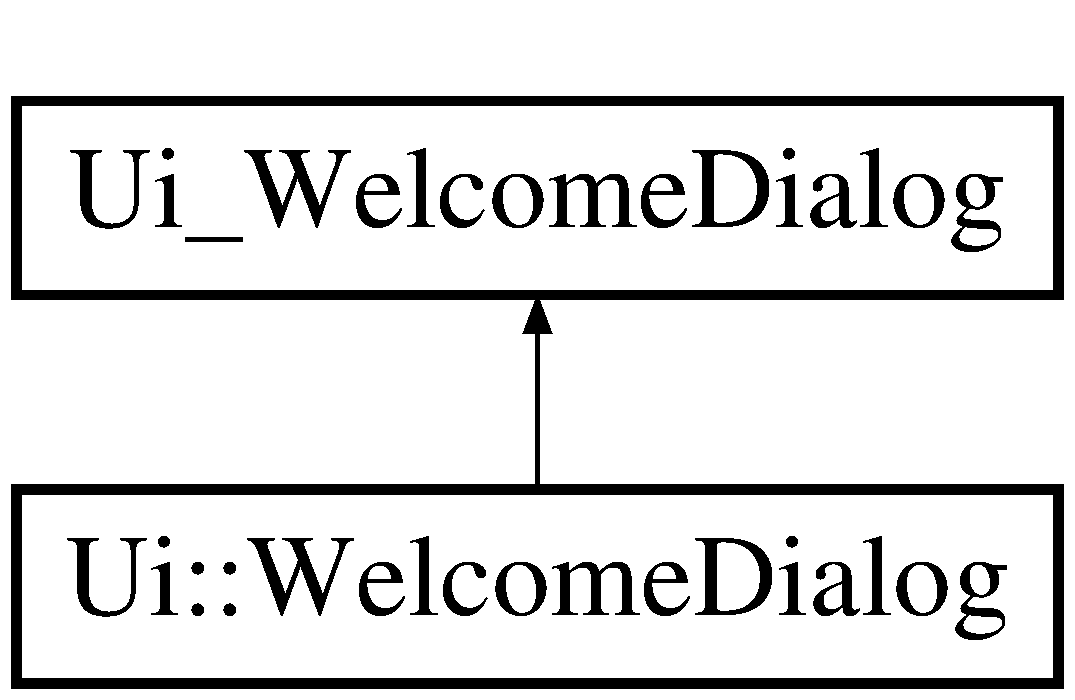
\includegraphics[height=2.000000cm]{class_ui_1_1_welcome_dialog}
\end{center}
\end{figure}
\subsection*{Additional Inherited Members}


The documentation for this class was generated from the following file\+:\begin{DoxyCompactItemize}
\item 
\hyperlink{ui__welcomedialog_8h}{ui\+\_\+welcomedialog.\+h}\end{DoxyCompactItemize}

\hypertarget{class_welcome_dialog}{}\section{Welcome\+Dialog Class Reference}
\label{class_welcome_dialog}\index{Welcome\+Dialog@{Welcome\+Dialog}}


The \hyperlink{class_welcome_dialog}{Welcome\+Dialog} class.  




{\ttfamily \#include $<$welcomedialog.\+h$>$}

Inheritance diagram for Welcome\+Dialog\+:\begin{figure}[H]
\begin{center}
\leavevmode
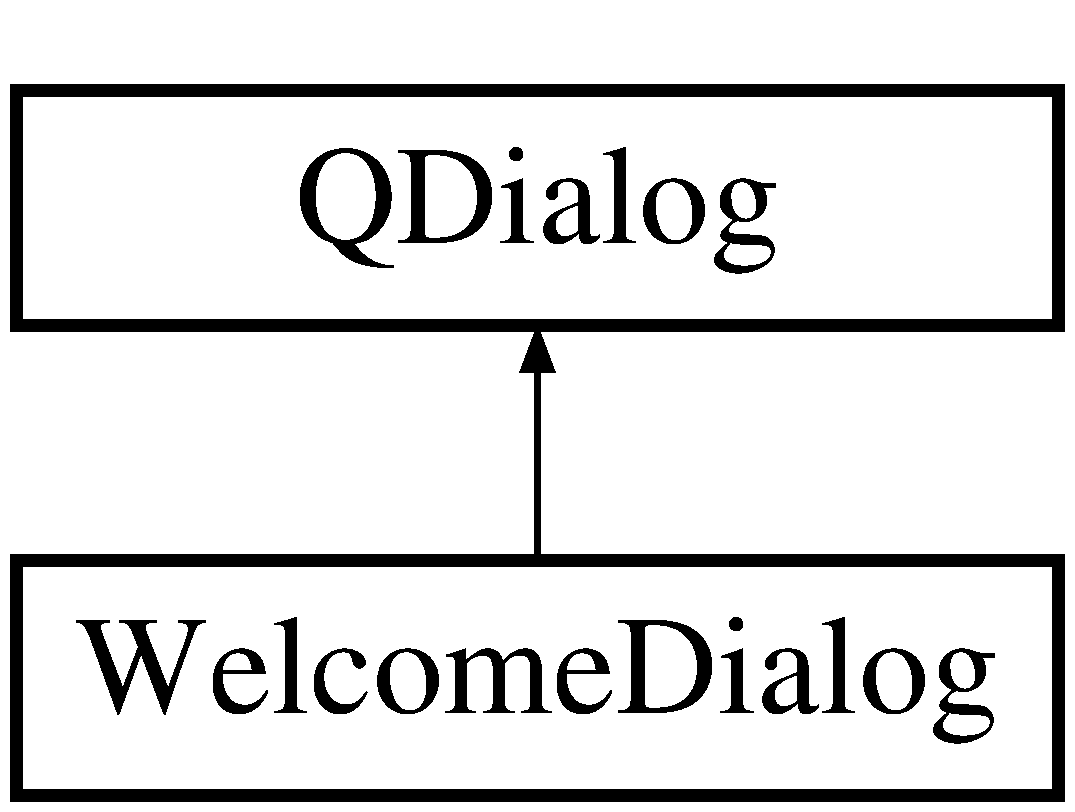
\includegraphics[height=2.000000cm]{class_welcome_dialog}
\end{center}
\end{figure}
\subsection*{Signals}
\begin{DoxyCompactItemize}
\item 
void \hyperlink{class_welcome_dialog_a13b5b9dd60876c39de70703d75949710}{show\+Line\+Tutorial\+Click} ()
\end{DoxyCompactItemize}
\subsection*{Public Member Functions}
\begin{DoxyCompactItemize}
\item 
\hyperlink{class_welcome_dialog_a1841278dd21a0e135b6e14b65857d3bc}{Welcome\+Dialog} (Q\+Widget $\ast$parent=0)
\item 
\hyperlink{class_welcome_dialog_aff7416acdda782ac3196ae28ea2ebe80}{$\sim$\+Welcome\+Dialog} ()
\end{DoxyCompactItemize}


\subsection{Detailed Description}
The \hyperlink{class_welcome_dialog}{Welcome\+Dialog} class. 

\subsection{Constructor \& Destructor Documentation}
\mbox{\Hypertarget{class_welcome_dialog_a1841278dd21a0e135b6e14b65857d3bc}\label{class_welcome_dialog_a1841278dd21a0e135b6e14b65857d3bc}} 
\index{Welcome\+Dialog@{Welcome\+Dialog}!Welcome\+Dialog@{Welcome\+Dialog}}
\index{Welcome\+Dialog@{Welcome\+Dialog}!Welcome\+Dialog@{Welcome\+Dialog}}
\subsubsection{\texorpdfstring{Welcome\+Dialog()}{WelcomeDialog()}}
{\footnotesize\ttfamily Welcome\+Dialog\+::\+Welcome\+Dialog (\begin{DoxyParamCaption}\item[{Q\+Widget $\ast$}]{parent = {\ttfamily 0} }\end{DoxyParamCaption})\hspace{0.3cm}{\ttfamily [explicit]}}

\mbox{\Hypertarget{class_welcome_dialog_aff7416acdda782ac3196ae28ea2ebe80}\label{class_welcome_dialog_aff7416acdda782ac3196ae28ea2ebe80}} 
\index{Welcome\+Dialog@{Welcome\+Dialog}!````~Welcome\+Dialog@{$\sim$\+Welcome\+Dialog}}
\index{````~Welcome\+Dialog@{$\sim$\+Welcome\+Dialog}!Welcome\+Dialog@{Welcome\+Dialog}}
\subsubsection{\texorpdfstring{$\sim$\+Welcome\+Dialog()}{~WelcomeDialog()}}
{\footnotesize\ttfamily Welcome\+Dialog\+::$\sim$\+Welcome\+Dialog (\begin{DoxyParamCaption}{ }\end{DoxyParamCaption})}



\subsection{Member Function Documentation}
\mbox{\Hypertarget{class_welcome_dialog_a13b5b9dd60876c39de70703d75949710}\label{class_welcome_dialog_a13b5b9dd60876c39de70703d75949710}} 
\index{Welcome\+Dialog@{Welcome\+Dialog}!show\+Line\+Tutorial\+Click@{show\+Line\+Tutorial\+Click}}
\index{show\+Line\+Tutorial\+Click@{show\+Line\+Tutorial\+Click}!Welcome\+Dialog@{Welcome\+Dialog}}
\subsubsection{\texorpdfstring{show\+Line\+Tutorial\+Click}{showLineTutorialClick}}
{\footnotesize\ttfamily void Welcome\+Dialog\+::show\+Line\+Tutorial\+Click (\begin{DoxyParamCaption}{ }\end{DoxyParamCaption})\hspace{0.3cm}{\ttfamily [signal]}}



The documentation for this class was generated from the following files\+:\begin{DoxyCompactItemize}
\item 
\hyperlink{welcomedialog_8h}{welcomedialog.\+h}\item 
\hyperlink{welcomedialog_8cpp}{welcomedialog.\+cpp}\end{DoxyCompactItemize}

\chapter{File Documentation}
\hypertarget{circle_8cpp}{}\section{circle.\+cpp File Reference}
\label{circle_8cpp}\index{circle.\+cpp@{circle.\+cpp}}
{\ttfamily \#include \char`\"{}circle.\+h\char`\"{}}\newline
{\ttfamily \#include $<$Q\+Pen$>$}\newline
{\ttfamily \#include $<$Q\+Brush$>$}\newline

\hypertarget{circle_8h}{}\section{circle.\+h File Reference}
\label{circle_8h}\index{circle.\+h@{circle.\+h}}
{\ttfamily \#include \char`\"{}graphicsobject.\+h\char`\"{}}\newline
{\ttfamily \#include $<$Q\+Object$>$}\newline
{\ttfamily \#include $<$Q\+String$>$}\newline
{\ttfamily \#include $<$Q\+Graphics\+Ellipse\+Item$>$}\newline
\subsection*{Classes}
\begin{DoxyCompactItemize}
\item 
class \hyperlink{class_circle}{Circle}
\begin{DoxyCompactList}\small\item\em The \hyperlink{class_circle}{Circle} class. \end{DoxyCompactList}\end{DoxyCompactItemize}

\hypertarget{colorbutton_8cpp}{}\section{colorbutton.\+cpp File Reference}
\label{colorbutton_8cpp}\index{colorbutton.\+cpp@{colorbutton.\+cpp}}
{\ttfamily \#include \char`\"{}colorbutton.\+h\char`\"{}}\newline
{\ttfamily \#include $<$Q\+Painter$>$}\newline
{\ttfamily \#include $<$Q\+String$>$}\newline
{\ttfamily \#include $<$Q\+Debug$>$}\newline

\hypertarget{colorbutton_8h}{}\section{colorbutton.\+h File Reference}
\label{colorbutton_8h}\index{colorbutton.\+h@{colorbutton.\+h}}
{\ttfamily \#include $<$Q\+Push\+Button$>$}\newline
\subsection*{Classes}
\begin{DoxyCompactItemize}
\item 
class \hyperlink{class_color_button}{Color\+Button}
\end{DoxyCompactItemize}

\hypertarget{colortoolselector_8cpp}{}\section{colortoolselector.\+cpp File Reference}
\label{colortoolselector_8cpp}\index{colortoolselector.\+cpp@{colortoolselector.\+cpp}}
{\ttfamily \#include \char`\"{}colortoolselector.\+h\char`\"{}}\newline
{\ttfamily \#include \char`\"{}ui\+\_\+colortoolselector.\+h\char`\"{}}\newline
{\ttfamily \#include $<$Q\+Color\+Dialog$>$}\newline
{\ttfamily \#include $<$Qt\+Debug$>$}\newline

\hypertarget{colortoolselector_8h}{}\section{colortoolselector.\+h File Reference}
\label{colortoolselector_8h}\index{colortoolselector.\+h@{colortoolselector.\+h}}
{\ttfamily \#include $<$Q\+Widget$>$}\newline
{\ttfamily \#include \char`\"{}draw.\+h\char`\"{}}\newline
\subsection*{Classes}
\begin{DoxyCompactItemize}
\item 
class \hyperlink{class_color_tool_selector}{Color\+Tool\+Selector}
\end{DoxyCompactItemize}
\subsection*{Namespaces}
\begin{DoxyCompactItemize}
\item 
 \hyperlink{namespace_ui}{Ui}
\end{DoxyCompactItemize}

\hypertarget{draw_8cpp}{}\section{draw.\+cpp File Reference}
\label{draw_8cpp}\index{draw.\+cpp@{draw.\+cpp}}
{\ttfamily \#include \char`\"{}draw.\+h\char`\"{}}\newline

\hypertarget{draw_8h}{}\section{draw.\+h File Reference}
\label{draw_8h}\index{draw.\+h@{draw.\+h}}
{\ttfamily \#include $<$Q\+Object$>$}\newline
{\ttfamily \#include $<$Q\+Color$>$}\newline
\subsection*{Classes}
\begin{DoxyCompactItemize}
\item 
class \hyperlink{class_draw}{Draw}
\end{DoxyCompactItemize}

\hypertarget{drawingtoolselector_8cpp}{}\section{drawingtoolselector.\+cpp File Reference}
\label{drawingtoolselector_8cpp}\index{drawingtoolselector.\+cpp@{drawingtoolselector.\+cpp}}
{\ttfamily \#include \char`\"{}drawingtoolselector.\+h\char`\"{}}\newline
{\ttfamily \#include \char`\"{}ui\+\_\+drawingtoolselector.\+h\char`\"{}}\newline

\hypertarget{drawingtoolselector_8h}{}\section{drawingtoolselector.\+h File Reference}
\label{drawingtoolselector_8h}\index{drawingtoolselector.\+h@{drawingtoolselector.\+h}}
{\ttfamily \#include $<$Q\+Widget$>$}\newline
{\ttfamily \#include $<$draw.\+h$>$}\newline
\subsection*{Classes}
\begin{DoxyCompactItemize}
\item 
class \hyperlink{class_drawing_tool_selector}{Drawing\+Tool\+Selector}
\begin{DoxyCompactList}\small\item\em The \hyperlink{class_drawing_tool_selector}{Drawing\+Tool\+Selector} class. \end{DoxyCompactList}\end{DoxyCompactItemize}
\subsection*{Namespaces}
\begin{DoxyCompactItemize}
\item 
 \hyperlink{namespace_ui}{Ui}
\end{DoxyCompactItemize}

\hypertarget{graphicsobject_8cpp}{}\section{graphicsobject.\+cpp File Reference}
\label{graphicsobject_8cpp}\index{graphicsobject.\+cpp@{graphicsobject.\+cpp}}
{\ttfamily \#include \char`\"{}graphicsobject.\+h\char`\"{}}\newline
{\ttfamily \#include $<$Q\+Object$>$}\newline
{\ttfamily \#include $<$iostream$>$}\newline
{\ttfamily \#include $<$Q\+Debug$>$}\newline

\hypertarget{graphicsobject_8h}{}\section{graphicsobject.\+h File Reference}
\label{graphicsobject_8h}\index{graphicsobject.\+h@{graphicsobject.\+h}}
{\ttfamily \#include $<$Q\+Object$>$}\newline
{\ttfamily \#include $<$Q\+String$>$}\newline
{\ttfamily \#include $<$Q\+Graphics\+Object$>$}\newline
{\ttfamily \#include $<$Q\+Graphics\+Scene$>$}\newline
{\ttfamily \#include $<$Q\+Graphics\+Scene\+Mouse\+Event$>$}\newline
{\ttfamily \#include $<$Q\+Graphics\+Item$>$}\newline
\subsection*{Classes}
\begin{DoxyCompactItemize}
\item 
class \hyperlink{class_graphics_object}{Graphics\+Object}
\begin{DoxyCompactList}\small\item\em The \hyperlink{class_graphics_object}{Graphics\+Object} class. \end{DoxyCompactList}\end{DoxyCompactItemize}

\hypertarget{graphicsobjectmap_8cpp}{}\section{graphicsobjectmap.\+cpp File Reference}
\label{graphicsobjectmap_8cpp}\index{graphicsobjectmap.\+cpp@{graphicsobjectmap.\+cpp}}
{\ttfamily \#include \char`\"{}graphicsobjectmap.\+h\char`\"{}}\newline
{\ttfamily \#include $<$Q\+Debug$>$}\newline

\hypertarget{graphicsobjectmap_8h}{}\section{graphicsobjectmap.\+h File Reference}
\label{graphicsobjectmap_8h}\index{graphicsobjectmap.\+h@{graphicsobjectmap.\+h}}
{\ttfamily \#include $<$Q\+Map$>$}\newline
{\ttfamily \#include $<$Q\+Graphics\+Item$>$}\newline
{\ttfamily \#include \char`\"{}graphicsobject.\+h\char`\"{}}\newline
\subsection*{Classes}
\begin{DoxyCompactItemize}
\item 
class \hyperlink{class_graphics_object_map}{Graphics\+Object\+Map}
\end{DoxyCompactItemize}

\hypertarget{graphicsscene_8cpp}{}\section{graphicsscene.\+cpp File Reference}
\label{graphicsscene_8cpp}\index{graphicsscene.\+cpp@{graphicsscene.\+cpp}}
{\ttfamily \#include \char`\"{}graphicsscene.\+h\char`\"{}}\newline
{\ttfamily \#include $<$Q\+Graphics\+Scene\+Mouse\+Event$>$}\newline
{\ttfamily \#include $<$iostream$>$}\newline
{\ttfamily \#include $<$Qt\+Debug$>$}\newline
{\ttfamily \#include $<$Q\+String$>$}\newline
{\ttfamily \#include \char`\"{}roomgroundplan.\+h\char`\"{}}\newline
{\ttfamily \#include \char`\"{}mainwindow.\+h\char`\"{}}\newline
{\ttfamily \#include \char`\"{}draw.\+h\char`\"{}}\newline
{\ttfamily \#include $<$Q\+Painter\+Path$>$}\newline
{\ttfamily \#include $<$Q\+Tool\+Tip$>$}\newline

\hypertarget{graphicsscene_8h}{}\section{graphicsscene.\+h File Reference}
\label{graphicsscene_8h}\index{graphicsscene.\+h@{graphicsscene.\+h}}
{\ttfamily \#include $<$qgraphicsscene.\+h$>$}\newline
{\ttfamily \#include \char`\"{}roomgroundplan.\+h\char`\"{}}\newline
{\ttfamily \#include \char`\"{}graphicsobject.\+h\char`\"{}}\newline
{\ttfamily \#include \char`\"{}graphicsobjectmap.\+h\char`\"{}}\newline
{\ttfamily \#include \char`\"{}draw.\+h\char`\"{}}\newline
{\ttfamily \#include $<$Q\+Tool\+Tip$>$}\newline
\subsection*{Classes}
\begin{DoxyCompactItemize}
\item 
class \hyperlink{class_graphics_scene}{Graphics\+Scene}
\begin{DoxyCompactList}\small\item\em The \hyperlink{class_graphics_scene}{Graphics\+Scene} class. \end{DoxyCompactList}\end{DoxyCompactItemize}

\hypertarget{main_8cpp}{}\section{main.\+cpp File Reference}
\label{main_8cpp}\index{main.\+cpp@{main.\+cpp}}
{\ttfamily \#include \char`\"{}mainwindow.\+h\char`\"{}}\newline
{\ttfamily \#include \char`\"{}welcomedialog.\+h\char`\"{}}\newline
{\ttfamily \#include $<$Q\+Application$>$}\newline
\subsection*{Functions}
\begin{DoxyCompactItemize}
\item 
int \hyperlink{main_8cpp_a0ddf1224851353fc92bfbff6f499fa97}{main} (int argc, char $\ast$argv\mbox{[}$\,$\mbox{]})
\end{DoxyCompactItemize}


\subsection{Function Documentation}
\mbox{\Hypertarget{main_8cpp_a0ddf1224851353fc92bfbff6f499fa97}\label{main_8cpp_a0ddf1224851353fc92bfbff6f499fa97}} 
\index{main.\+cpp@{main.\+cpp}!main@{main}}
\index{main@{main}!main.\+cpp@{main.\+cpp}}
\subsubsection{\texorpdfstring{main()}{main()}}
{\footnotesize\ttfamily int main (\begin{DoxyParamCaption}\item[{int}]{argc,  }\item[{char $\ast$}]{argv\mbox{[}$\,$\mbox{]} }\end{DoxyParamCaption})}


\hypertarget{mainwindow_8cpp}{}\section{mainwindow.\+cpp File Reference}
\label{mainwindow_8cpp}\index{mainwindow.\+cpp@{mainwindow.\+cpp}}
{\ttfamily \#include \char`\"{}mainwindow.\+h\char`\"{}}\newline
{\ttfamily \#include \char`\"{}ui\+\_\+mainwindow.\+h\char`\"{}}\newline
{\ttfamily \#include \char`\"{}qgraphicsscene.\+h\char`\"{}}\newline
{\ttfamily \#include $<$iostream$>$}\newline
{\ttfamily \#include $<$Q\+String$>$}\newline
{\ttfamily \#include $<$draw.\+h$>$}\newline
{\ttfamily \#include $<$Qt\+Debug$>$}\newline
{\ttfamily \#include $<$Q\+Color\+Dialog$>$}\newline
{\ttfamily \#include $<$Q\+Color$>$}\newline
{\ttfamily \#include $<$Q\+Graphics\+Scene\+Mouse\+Event$>$}\newline
{\ttfamily \#include $<$Q\+Graphics\+Item$>$}\newline
{\ttfamily \#include \char`\"{}objectsettings.\+h\char`\"{}}\newline

\hypertarget{mainwindow_8h}{}\section{mainwindow.\+h File Reference}
\label{mainwindow_8h}\index{mainwindow.\+h@{mainwindow.\+h}}
{\ttfamily \#include $<$Q\+Main\+Window$>$}\newline
{\ttfamily \#include $<$Q\+String$>$}\newline
{\ttfamily \#include \char`\"{}rectangle.\+h\char`\"{}}\newline
{\ttfamily \#include \char`\"{}circle.\+h\char`\"{}}\newline
{\ttfamily \#include \char`\"{}draw.\+h\char`\"{}}\newline
{\ttfamily \#include \char`\"{}graphicsobjectmap.\+h\char`\"{}}\newline
{\ttfamily \#include \char`\"{}graphicsscene.\+h\char`\"{}}\newline
{\ttfamily \#include \char`\"{}colorbutton.\+h\char`\"{}}\newline
{\ttfamily \#include \char`\"{}graphicsobject.\+h\char`\"{}}\newline
{\ttfamily \#include \char`\"{}objectsettings.\+h\char`\"{}}\newline
{\ttfamily \#include \char`\"{}tutoriallinetool.\+h\char`\"{}}\newline
\subsection*{Classes}
\begin{DoxyCompactItemize}
\item 
class \hyperlink{class_main_window}{Main\+Window}
\end{DoxyCompactItemize}
\subsection*{Namespaces}
\begin{DoxyCompactItemize}
\item 
 \hyperlink{namespace_ui}{Ui}
\end{DoxyCompactItemize}

\hypertarget{objectsettings_8cpp}{}\section{objectsettings.\+cpp File Reference}
\label{objectsettings_8cpp}\index{objectsettings.\+cpp@{objectsettings.\+cpp}}
{\ttfamily \#include \char`\"{}objectsettings.\+h\char`\"{}}\newline
{\ttfamily \#include \char`\"{}ui\+\_\+objectsettings.\+h\char`\"{}}\newline
{\ttfamily \#include \char`\"{}mainwindow.\+h\char`\"{}}\newline
{\ttfamily \#include $<$iostream$>$}\newline
{\ttfamily \#include $<$Q\+Debug$>$}\newline

\hypertarget{objectsettings_8h}{}\section{objectsettings.\+h File Reference}
\label{objectsettings_8h}\index{objectsettings.\+h@{objectsettings.\+h}}
{\ttfamily \#include $<$Q\+Widget$>$}\newline
{\ttfamily \#include \char`\"{}graphicsobject.\+h\char`\"{}}\newline
\subsection*{Classes}
\begin{DoxyCompactItemize}
\item 
class \hyperlink{class_object_settings}{Object\+Settings}
\begin{DoxyCompactList}\small\item\em The \hyperlink{class_object_settings}{Object\+Settings} class. \end{DoxyCompactList}\end{DoxyCompactItemize}
\subsection*{Namespaces}
\begin{DoxyCompactItemize}
\item 
 \hyperlink{namespace_ui}{Ui}
\end{DoxyCompactItemize}

\hypertarget{rectangle_8cpp}{}\section{rectangle.\+cpp File Reference}
\label{rectangle_8cpp}\index{rectangle.\+cpp@{rectangle.\+cpp}}
{\ttfamily \#include \char`\"{}rectangle.\+h\char`\"{}}\newline
{\ttfamily \#include $<$Q\+Pen$>$}\newline
{\ttfamily \#include $<$Q\+Brush$>$}\newline

\hypertarget{rectangle_8h}{}\section{rectangle.\+h File Reference}
\label{rectangle_8h}\index{rectangle.\+h@{rectangle.\+h}}
{\ttfamily \#include \char`\"{}graphicsobject.\+h\char`\"{}}\newline
{\ttfamily \#include $<$Q\+Object$>$}\newline
{\ttfamily \#include $<$Q\+String$>$}\newline
{\ttfamily \#include $<$Q\+Graphics\+Rect\+Item$>$}\newline
\subsection*{Classes}
\begin{DoxyCompactItemize}
\item 
class \hyperlink{class_rectangle}{Rectangle}
\begin{DoxyCompactList}\small\item\em The \hyperlink{class_rectangle}{Rectangle} class. \end{DoxyCompactList}\end{DoxyCompactItemize}

\hypertarget{roomgroundplan_8cpp}{}\section{roomgroundplan.\+cpp File Reference}
\label{roomgroundplan_8cpp}\index{roomgroundplan.\+cpp@{roomgroundplan.\+cpp}}
{\ttfamily \#include \char`\"{}roomgroundplan.\+h\char`\"{}}\newline
{\ttfamily \#include $<$Q\+Graphics\+Line\+Item$>$}\newline
{\ttfamily \#include $<$Q\+Debug$>$}\newline

\hypertarget{roomgroundplan_8h}{}\section{roomgroundplan.\+h File Reference}
\label{roomgroundplan_8h}\index{roomgroundplan.\+h@{roomgroundplan.\+h}}
{\ttfamily \#include $<$Q\+Object$>$}\newline
{\ttfamily \#include $<$Q\+Graphics\+Item\+Group$>$}\newline
\subsection*{Classes}
\begin{DoxyCompactItemize}
\item 
class \hyperlink{class_room_groundplan}{Room\+Groundplan}
\begin{DoxyCompactList}\small\item\em The \hyperlink{class_room_groundplan}{Room\+Groundplan} class. \end{DoxyCompactList}\end{DoxyCompactItemize}

\hypertarget{tutoriallinetool_8cpp}{}\section{tutoriallinetool.\+cpp File Reference}
\label{tutoriallinetool_8cpp}\index{tutoriallinetool.\+cpp@{tutoriallinetool.\+cpp}}
{\ttfamily \#include \char`\"{}tutoriallinetool.\+h\char`\"{}}\newline
{\ttfamily \#include \char`\"{}ui\+\_\+tutoriallinetool.\+h\char`\"{}}\newline

\hypertarget{tutoriallinetool_8h}{}\section{tutoriallinetool.\+h File Reference}
\label{tutoriallinetool_8h}\index{tutoriallinetool.\+h@{tutoriallinetool.\+h}}
{\ttfamily \#include $<$Q\+Dialog$>$}\newline
\subsection*{Classes}
\begin{DoxyCompactItemize}
\item 
class \hyperlink{class_tutorial_line_tool}{Tutorial\+Line\+Tool}
\begin{DoxyCompactList}\small\item\em The \hyperlink{class_tutorial_line_tool}{Tutorial\+Line\+Tool} class. \end{DoxyCompactList}\end{DoxyCompactItemize}
\subsection*{Namespaces}
\begin{DoxyCompactItemize}
\item 
 \hyperlink{namespace_ui}{Ui}
\end{DoxyCompactItemize}

\hypertarget{ui__colortoolselector_8h}{}\section{ui\+\_\+colortoolselector.\+h File Reference}
\label{ui__colortoolselector_8h}\index{ui\+\_\+colortoolselector.\+h@{ui\+\_\+colortoolselector.\+h}}
{\ttfamily \#include $<$Qt\+Core/\+Q\+Variant$>$}\newline
{\ttfamily \#include $<$Qt\+Widgets/\+Q\+Action$>$}\newline
{\ttfamily \#include $<$Qt\+Widgets/\+Q\+Application$>$}\newline
{\ttfamily \#include $<$Qt\+Widgets/\+Q\+Button\+Group$>$}\newline
{\ttfamily \#include $<$Qt\+Widgets/\+Q\+Grid\+Layout$>$}\newline
{\ttfamily \#include $<$Qt\+Widgets/\+Q\+Group\+Box$>$}\newline
{\ttfamily \#include $<$Qt\+Widgets/\+Q\+Header\+View$>$}\newline
{\ttfamily \#include $<$Qt\+Widgets/\+Q\+V\+Box\+Layout$>$}\newline
{\ttfamily \#include $<$Qt\+Widgets/\+Q\+Widget$>$}\newline
{\ttfamily \#include \char`\"{}colorbutton.\+h\char`\"{}}\newline
\subsection*{Classes}
\begin{DoxyCompactItemize}
\item 
class \hyperlink{class_ui___color_tool_selector}{Ui\+\_\+\+Color\+Tool\+Selector}
\item 
class \hyperlink{class_ui_1_1_color_tool_selector}{Ui\+::\+Color\+Tool\+Selector}
\end{DoxyCompactItemize}
\subsection*{Namespaces}
\begin{DoxyCompactItemize}
\item 
 \hyperlink{namespace_ui}{Ui}
\end{DoxyCompactItemize}

\hypertarget{ui__drawingtoolselector_8h}{}\section{ui\+\_\+drawingtoolselector.\+h File Reference}
\label{ui__drawingtoolselector_8h}\index{ui\+\_\+drawingtoolselector.\+h@{ui\+\_\+drawingtoolselector.\+h}}
{\ttfamily \#include $<$Qt\+Core/\+Q\+Variant$>$}\newline
{\ttfamily \#include $<$Qt\+Widgets/\+Q\+Action$>$}\newline
{\ttfamily \#include $<$Qt\+Widgets/\+Q\+Application$>$}\newline
{\ttfamily \#include $<$Qt\+Widgets/\+Q\+Button\+Group$>$}\newline
{\ttfamily \#include $<$Qt\+Widgets/\+Q\+Grid\+Layout$>$}\newline
{\ttfamily \#include $<$Qt\+Widgets/\+Q\+Group\+Box$>$}\newline
{\ttfamily \#include $<$Qt\+Widgets/\+Q\+Header\+View$>$}\newline
{\ttfamily \#include $<$Qt\+Widgets/\+Q\+Label$>$}\newline
{\ttfamily \#include $<$Qt\+Widgets/\+Q\+Tool\+Button$>$}\newline
{\ttfamily \#include $<$Qt\+Widgets/\+Q\+Widget$>$}\newline
\subsection*{Classes}
\begin{DoxyCompactItemize}
\item 
class \hyperlink{class_ui___drawing_tool_selector}{Ui\+\_\+\+Drawing\+Tool\+Selector}
\item 
class \hyperlink{class_ui_1_1_drawing_tool_selector}{Ui\+::\+Drawing\+Tool\+Selector}
\end{DoxyCompactItemize}
\subsection*{Namespaces}
\begin{DoxyCompactItemize}
\item 
 \hyperlink{namespace_ui}{Ui}
\end{DoxyCompactItemize}

\hypertarget{ui__mainwindow_8h}{}\section{ui\+\_\+mainwindow.\+h File Reference}
\label{ui__mainwindow_8h}\index{ui\+\_\+mainwindow.\+h@{ui\+\_\+mainwindow.\+h}}
{\ttfamily \#include $<$Qt\+Core/\+Q\+Variant$>$}\newline
{\ttfamily \#include $<$Qt\+Widgets/\+Q\+Action$>$}\newline
{\ttfamily \#include $<$Qt\+Widgets/\+Q\+Application$>$}\newline
{\ttfamily \#include $<$Qt\+Widgets/\+Q\+Button\+Group$>$}\newline
{\ttfamily \#include $<$Qt\+Widgets/\+Q\+Double\+Spin\+Box$>$}\newline
{\ttfamily \#include $<$Qt\+Widgets/\+Q\+Graphics\+View$>$}\newline
{\ttfamily \#include $<$Qt\+Widgets/\+Q\+Grid\+Layout$>$}\newline
{\ttfamily \#include $<$Qt\+Widgets/\+Q\+Group\+Box$>$}\newline
{\ttfamily \#include $<$Qt\+Widgets/\+Q\+H\+Box\+Layout$>$}\newline
{\ttfamily \#include $<$Qt\+Widgets/\+Q\+Header\+View$>$}\newline
{\ttfamily \#include $<$Qt\+Widgets/\+Q\+Label$>$}\newline
{\ttfamily \#include $<$Qt\+Widgets/\+Q\+Main\+Window$>$}\newline
{\ttfamily \#include $<$Qt\+Widgets/\+Q\+Menu$>$}\newline
{\ttfamily \#include $<$Qt\+Widgets/\+Q\+Menu\+Bar$>$}\newline
{\ttfamily \#include $<$Qt\+Widgets/\+Q\+Push\+Button$>$}\newline
{\ttfamily \#include $<$Qt\+Widgets/\+Q\+Spin\+Box$>$}\newline
{\ttfamily \#include $<$Qt\+Widgets/\+Q\+Status\+Bar$>$}\newline
{\ttfamily \#include $<$Qt\+Widgets/\+Q\+Tool\+Bar$>$}\newline
{\ttfamily \#include $<$Qt\+Widgets/\+Q\+Widget$>$}\newline
{\ttfamily \#include \char`\"{}colortoolselector.\+h\char`\"{}}\newline
{\ttfamily \#include \char`\"{}drawingtoolselector.\+h\char`\"{}}\newline
{\ttfamily \#include \char`\"{}objectsettings.\+h\char`\"{}}\newline
\subsection*{Classes}
\begin{DoxyCompactItemize}
\item 
class \hyperlink{class_ui___main_window}{Ui\+\_\+\+Main\+Window}
\item 
class \hyperlink{class_ui_1_1_main_window}{Ui\+::\+Main\+Window}
\end{DoxyCompactItemize}
\subsection*{Namespaces}
\begin{DoxyCompactItemize}
\item 
 \hyperlink{namespace_ui}{Ui}
\end{DoxyCompactItemize}

\hypertarget{ui__objectsettings_8h}{}\section{ui\+\_\+objectsettings.\+h File Reference}
\label{ui__objectsettings_8h}\index{ui\+\_\+objectsettings.\+h@{ui\+\_\+objectsettings.\+h}}
{\ttfamily \#include $<$Qt\+Core/\+Q\+Variant$>$}\newline
{\ttfamily \#include $<$Qt\+Widgets/\+Q\+Action$>$}\newline
{\ttfamily \#include $<$Qt\+Widgets/\+Q\+Application$>$}\newline
{\ttfamily \#include $<$Qt\+Widgets/\+Q\+Button\+Group$>$}\newline
{\ttfamily \#include $<$Qt\+Widgets/\+Q\+Dial$>$}\newline
{\ttfamily \#include $<$Qt\+Widgets/\+Q\+Group\+Box$>$}\newline
{\ttfamily \#include $<$Qt\+Widgets/\+Q\+H\+Box\+Layout$>$}\newline
{\ttfamily \#include $<$Qt\+Widgets/\+Q\+Header\+View$>$}\newline
{\ttfamily \#include $<$Qt\+Widgets/\+Q\+Line\+Edit$>$}\newline
{\ttfamily \#include $<$Qt\+Widgets/\+Q\+Push\+Button$>$}\newline
{\ttfamily \#include $<$Qt\+Widgets/\+Q\+V\+Box\+Layout$>$}\newline
{\ttfamily \#include $<$Qt\+Widgets/\+Q\+Widget$>$}\newline
\subsection*{Classes}
\begin{DoxyCompactItemize}
\item 
class \hyperlink{class_ui___object_settings}{Ui\+\_\+\+Object\+Settings}
\item 
class \hyperlink{class_ui_1_1_object_settings}{Ui\+::\+Object\+Settings}
\end{DoxyCompactItemize}
\subsection*{Namespaces}
\begin{DoxyCompactItemize}
\item 
 \hyperlink{namespace_ui}{Ui}
\end{DoxyCompactItemize}

\hypertarget{ui__tutoriallinetool_8h}{}\section{ui\+\_\+tutoriallinetool.\+h File Reference}
\label{ui__tutoriallinetool_8h}\index{ui\+\_\+tutoriallinetool.\+h@{ui\+\_\+tutoriallinetool.\+h}}
{\ttfamily \#include $<$Qt\+Core/\+Q\+Variant$>$}\newline
{\ttfamily \#include $<$Qt\+Widgets/\+Q\+Action$>$}\newline
{\ttfamily \#include $<$Qt\+Widgets/\+Q\+Application$>$}\newline
{\ttfamily \#include $<$Qt\+Widgets/\+Q\+Button\+Group$>$}\newline
{\ttfamily \#include $<$Qt\+Widgets/\+Q\+Dialog$>$}\newline
{\ttfamily \#include $<$Qt\+Widgets/\+Q\+Dialog\+Button\+Box$>$}\newline
{\ttfamily \#include $<$Qt\+Widgets/\+Q\+Grid\+Layout$>$}\newline
{\ttfamily \#include $<$Qt\+Widgets/\+Q\+Group\+Box$>$}\newline
{\ttfamily \#include $<$Qt\+Widgets/\+Q\+Header\+View$>$}\newline
{\ttfamily \#include $<$Qt\+Widgets/\+Q\+Label$>$}\newline
{\ttfamily \#include $<$Qt\+Widgets/\+Q\+Push\+Button$>$}\newline
{\ttfamily \#include $<$Qt\+Widgets/\+Q\+Widget$>$}\newline
\subsection*{Classes}
\begin{DoxyCompactItemize}
\item 
class \hyperlink{class_ui___tutorial_line_tool}{Ui\+\_\+\+Tutorial\+Line\+Tool}
\item 
class \hyperlink{class_ui_1_1_tutorial_line_tool}{Ui\+::\+Tutorial\+Line\+Tool}
\end{DoxyCompactItemize}
\subsection*{Namespaces}
\begin{DoxyCompactItemize}
\item 
 \hyperlink{namespace_ui}{Ui}
\end{DoxyCompactItemize}

\hypertarget{ui__welcomedialog_8h}{}\section{ui\+\_\+welcomedialog.\+h File Reference}
\label{ui__welcomedialog_8h}\index{ui\+\_\+welcomedialog.\+h@{ui\+\_\+welcomedialog.\+h}}
{\ttfamily \#include $<$Qt\+Core/\+Q\+Variant$>$}\newline
{\ttfamily \#include $<$Qt\+Widgets/\+Q\+Action$>$}\newline
{\ttfamily \#include $<$Qt\+Widgets/\+Q\+Application$>$}\newline
{\ttfamily \#include $<$Qt\+Widgets/\+Q\+Button\+Group$>$}\newline
{\ttfamily \#include $<$Qt\+Widgets/\+Q\+Dialog$>$}\newline
{\ttfamily \#include $<$Qt\+Widgets/\+Q\+Dialog\+Button\+Box$>$}\newline
{\ttfamily \#include $<$Qt\+Widgets/\+Q\+Grid\+Layout$>$}\newline
{\ttfamily \#include $<$Qt\+Widgets/\+Q\+Header\+View$>$}\newline
{\ttfamily \#include $<$Qt\+Widgets/\+Q\+Label$>$}\newline
{\ttfamily \#include $<$Qt\+Widgets/\+Q\+Spacer\+Item$>$}\newline
{\ttfamily \#include $<$Qt\+Widgets/\+Q\+Widget$>$}\newline
\subsection*{Classes}
\begin{DoxyCompactItemize}
\item 
class \hyperlink{class_ui___welcome_dialog}{Ui\+\_\+\+Welcome\+Dialog}
\item 
class \hyperlink{class_ui_1_1_welcome_dialog}{Ui\+::\+Welcome\+Dialog}
\end{DoxyCompactItemize}
\subsection*{Namespaces}
\begin{DoxyCompactItemize}
\item 
 \hyperlink{namespace_ui}{Ui}
\end{DoxyCompactItemize}

\hypertarget{welcomedialog_8cpp}{}\section{welcomedialog.\+cpp File Reference}
\label{welcomedialog_8cpp}\index{welcomedialog.\+cpp@{welcomedialog.\+cpp}}
{\ttfamily \#include \char`\"{}welcomedialog.\+h\char`\"{}}\newline
{\ttfamily \#include \char`\"{}ui\+\_\+welcomedialog.\+h\char`\"{}}\newline
{\ttfamily \#include $<$iostream$>$}\newline
{\ttfamily \#include $<$Q\+Debug$>$}\newline

\hypertarget{welcomedialog_8h}{}\section{welcomedialog.\+h File Reference}
\label{welcomedialog_8h}\index{welcomedialog.\+h@{welcomedialog.\+h}}
{\ttfamily \#include $<$Q\+Dialog$>$}\newline
{\ttfamily \#include \char`\"{}tutoriallinetool.\+h\char`\"{}}\newline
\subsection*{Classes}
\begin{DoxyCompactItemize}
\item 
class \hyperlink{class_welcome_dialog}{Welcome\+Dialog}
\begin{DoxyCompactList}\small\item\em The \hyperlink{class_welcome_dialog}{Welcome\+Dialog} class. \end{DoxyCompactList}\end{DoxyCompactItemize}
\subsection*{Namespaces}
\begin{DoxyCompactItemize}
\item 
 \hyperlink{namespace_ui}{Ui}
\end{DoxyCompactItemize}

%--- End generated contents ---

% Index
\backmatter
\newpage
\phantomsection
\clearemptydoublepage
\addcontentsline{toc}{chapter}{Index}
\printindex

\end{document}
